\documentclass[11pt]{article}
\usepackage[margin=0.8in]{geometry}
\usepackage[utf8]{inputenc}
\usepackage{amsmath}
\usepackage{amssymb}
\usepackage{graphicx}
\usepackage{dirtytalk}
\usepackage{hyperref}
\usepackage{floatrow}
\usepackage{booktabs}
\usepackage{soul}
\usepackage{adjustbox}
\floatsetup[table]{capposition=bottom}
\usepackage{authblk}
\usepackage{lscape}
\usepackage{threeparttable}
\usepackage[official]{eurosym}
\usepackage{mwe}
\usepackage{fancyhdr}
\pagestyle{fancy}
\usepackage{xurl}

% Clear default header/footer
\fancyhf{}
\newcommand{\reviewername}{Reviewer 1} % Default value

\usepackage{acro}
\usepackage[toc,page]{appendix}
\usepackage{caption}
\usepackage{subcaption}
\usepackage{lineno}
\usepackage{siunitx}
\usepackage{comment}
\usepackage{xcolor}
\usepackage{makecell}
% \usepackage[numbers]{natbib} 
\usepackage[authoryear]{natbib}
\usepackage[noabbrev, capitalise]{cleveref}
\usepackage{tabularx}
\usepackage{colortbl}
\usepackage{tabulary}
\usepackage{etoolbox}
\usepackage{ifthen}
\usepackage{rotating}
\usepackage{bbding}
\usepackage{pgfplots}
\usepackage{enumitem}
\usepackage{tikzsymbols}
\usepackage{threeparttable}
\usepackage{multirow}
\usepackage{graphicx}
\usepackage{array}
\usepackage{colortbl}
\usepackage{threeparttable}
\newcolumntype{L}[1]{>{\raggedright\arraybackslash}p{#1}}

\definecolor{authorblue}{HTML}{2176ff}
\definecolor{reviewergrey}{HTML}{252323} % 495057

%\usepackage[markup=underlined, commandnameprefix=ifneeded]{changes}
\usepackage[final, commandnameprefix=ifneeded]{changes}
% \added{neuer Text} \deleted{zu löschender text} \replaced{neu}{alt}

\acsetup{first-style=short}

\renewcommand{\footnotesize}{\tiny}

\newcounter{reviewcounter}

\newcommand{\reviewersresponse}[7]{%
    \stepcounter{reviewcounter}
    \noindent \arabic{reviewcounter}) \textbf{#1} 
    \noindent\hangindent=1.5em\hangafter=1
    \begin{itemize} % adjust the amount of reviewers and their respective number
        \item \textit{\textcolor{reviewergrey}{\textbf{Reviewer 1:} #2}}
        \item \textit{\textcolor{reviewergrey}{\textbf{Reviewer 2:} #3}}
        \item \textit{\textcolor{reviewergrey}{\textbf{Reviewer 3:} #4}}
    \end{itemize}
    \textcolor{authorblue}{\textbf{Author's response:} #5} % #X should be changed depending on the number of reviewers
    \vspace{0.5cm}
}

\newcommand{\review}[2]{%
    \stepcounter{reviewcounter}% Erhöht den Zähler
    \noindent\hangindent=1.5em\hangafter=1%
    \textit{\textcolor{reviewergrey}{\arabic{reviewcounter}) #1}} \\[0.5em]
    \textcolor{authorblue}{\textbf{Author's response:} #2} \vspace{0.3cm}
}

\begin{document}
\fancyfoot[C]{\thepage}
\noindent To the editor and reviewers, \\

Thank you for considering our manuscript for publication in \textit{Transportation Research Part D: Transport and Environment}. We sincerely appreciate the time and effort of the editor and reviewers in providing their insightful comments and constructive feedback. In your comments, valid concerns and important issues have been raised, which have helped to improve the quality of the manuscript. 

The reviewers provided several overlapping comments, many of which focused on similar issues. Collectively, their feedback emphasized the need to prove the robustness of our findings.\\

\noindent We have addressed this at two levels:

\begin{itemize}
    \item Strengthening the empirical justification for our data assumptions through more detailed reasoning and support.
    \item Expanding our analysis of model sensitivities to demonstrate the robustness of our findings.
\end{itemize}

\noindent We have addressed these comments in point-by-point responses with corresponding references to the manuscript. Changes in the manuscript are highlighted with text color \textcolor{blue}{\textbf{blue}}, and each response explicitly indicates where the associated changes can be found. We believe that addressing the reviewers' concerns has strengthened the quality and clarity of our contribution to the research community.
We hope that these revisions render the manuscript well suited for publication in \textit{Transport Research Part D: Transport and Environment}.
\vspace{0.5cm}


% \noindent We have made a concerted effort to incorporate all provided comments and concerns. We believe these revision rounds have significantly improved the quality and clarity of the manuscript, making it more suitable for publication in \textit{JOURNAL}.

\newpage
\fancyhead[L]{\textit{Response to Reviewer \#1}}
\section*{\textit{Reviewer's Responses to Comments}}
\section*{Reviewer \#1}
\textbf{The paper develops a techno-economic network-design optimization (LP + a mixed-integer extension) that endogenously links public charging capacity expansion with an explicit detour fueling time variable and differentiates consumers by income quintiles (VoT, budgets, home-ownership). It studies two stylized roll-out strategies (distributed vs concentrated densification) and the speed of roll-out (accelerated vs slowed neighbors) using a Basque Country case study to address (1) how spatial densification affects BEV adoption across income classes and (2) whether rapid local expansion spills over to neighboring regions. Main findings: network densification materially alters charger usage patterns across income classes and fast, local expansion produces small positive spillovers on neighboring BEV adoption (max 1.3 percentage-point increase in electrification share).} \\

\color{reviewergrey}
\subsubsection*{Major strengths}
\textbf{
\begin{itemize}
    \item Novel linkage of infrastructure design and detour time: Introducing detour time as an endogenous variable tied to discrete capacity "lumps" is an interesting way to capture service level changes without fully spatially explicit siting.
    \item Income-class differentiation: Explicitly modeling five income quintiles with different VoT, budgets and home-charging access adds important behavioral realism and equity insights.
    \item Clear scenario framework that isolates density vs speed effects: The distributed vs concentrated and the accelerated vs slowed neighbor scenarios are well motivated and transparently implemented.
    \item Good technical implementation: The model is implemented in JuMP/Gurobi and the authors note computational details; this supports replicability (although see reproducibility comment).
\end{itemize}}

\color{authorblue}
\noindent \textcolor{authorblue}{\textbf{Author's response:}} Thank you for your time spent reviewing our manuscript. Your detailed comments and concrete recommendations have greatly helped improve its quality.
\newpage
\color{reviewergrey}

\subsubsection*{Major weaknesses / required revisions (actionable)}

\subsubsection*{1. Calibration and empirical grounding of the detour function g(q) and spatial assumptions \\
\textbf{Issue}: The paper assumes an even spatial distribution of chargers within NUTS regions and translates installed capacity → number of sites → areal spacing → detour time (Equations 9-12). This strong simplifying assumption is acknowledged by the authors but is also central to the results. The shape and parameters of the detour reduction curves (including the imposed minimum 5-minute detour) drive RQ1 results (Figures 4, detour/time plots).\\
\textbf{Required:} Provide empirical or synthetic calibration and sensitivity tests for g(q). Suggested steps:\\
\begin{itemize}
    \item[a.]Calibrate g(q) with an empirical dataset (e.g., geo-locations of existing chargers & road network distances) or at least compare the assumed curve with sampled synthetic siting (Monte Carlo placing chargers) so readers can see whether the assumed reduction curve is realistic for the Basque road/urban structure.
    \item[b.] Present sensitivity results for at least two alternative g(·) shapes (e.g., diminishing returns vs piecewise linear) and show how sensitive BEV adoption and utilization patterns are to those shapes.
    \item[c.] Discuss the bias introduced by the even-distribution assumption and indicate whether the results (especially cross-income effects) hold under more clustered (urban-targeted) siting.
\end{itemize}
\textbf{References in manuscript}: authors already flag this as a limitation; please move from "limitation" to concrete testing.
}\newline
\color{authorblue}
\noindent {\textbf{Author's response:}} Thank you for highlighting this point and the detailed elaboration of this limitation. We agree that the formulation of this function plays a central role to the conclusion of the manuscript. In the following, we \textbf{justify the formulation of the function} and \textbf{describe conducted sensitivity analyses}.

The detour fueling time function $g(q^{fuel\_infr, +})$ relates the expansion of public charging infrastructure to the decrease in average detouring time, i.e. the time needed to reach the closest charging station. It is introduced to express the increasing density of the charger network and the therein decreased time that is spent for the charging activity. This is a key contribution of our work to the state of the art: it enables a high-level representation of information that would otherwise require geographically fine-grained data and detailed vehicle-movement modeling, which typically requires a reduction in geographic scope. While this approach provides the advantages of reduced spatial resolution, it inherently overlooks heterogeneity within the region. We have presented different parameterizations of the detour fueling time function $g(q^{fuel\_infr, +})$ by introducing three scenarios on the numbers of charging points per site, i.e. $n^{\mathrm{points per site}} = 2$ \textit{(Distributed expansion)}, $n^{\mathrm{points per site}} = 10$ and $n^{\mathrm{points per site}} = 40$ \textit{(Centralized expansion)} (Section 4.1). Based on this, we observed changes in the cost-optimal charging utilization across income classes.

The key parameters defining the shape of the function are the region's area, the relative difference between Euclidean distance and detouring distance, the average travel speed and the installed charging capacity per site. A key assumption underlying this function is that charging sites are evenly distributed relative to the BEV driver’s location, as we model the \textit{average} detour-related fueling time.

As the reviewer notes in \textbf{point a. and b.}, calibrating the function using empirical data—for example, by sampling driving distances between randomly assigned origins and potential BEV driver locations—could indeed enhance the validity of the resulting shape of $g(q^{fuel\_infr, +})$. Rather than conducting such sampling ourselves, we build on existing literature on facility allocation, average distance minimization, and empirical distance distributions. This literature provides robust and well-established insights that support our assumptions and, in turn, support the plausibility of the functional form of $g(q^{fuel\_infr, +})$. 

We use the \textit{circuity} parameter which expresses the ratio between the Euclidean distance and the distance in the road network. In our analysis we assume this value to be 1.4.
The following figure displays measured values for different European cities which are drawn from a recent study by \citet{COSTA2025106087} together with the assumed value. In the Basque country, around 70\% of population lives in urban areas \citep{BasqueCountryPopulation2024}. The five minute threshold is based on an educated guess by the authors. This is based on the assumption that lower times for detouring (time required to reach the charging station \textbf{and} back from the charging station) are unrealistic. Further, a lower limit it is set to avoid very small values in the optimization which could lead to increased computational complexity in the solution of the MILP.

\begin{figure}[H]
    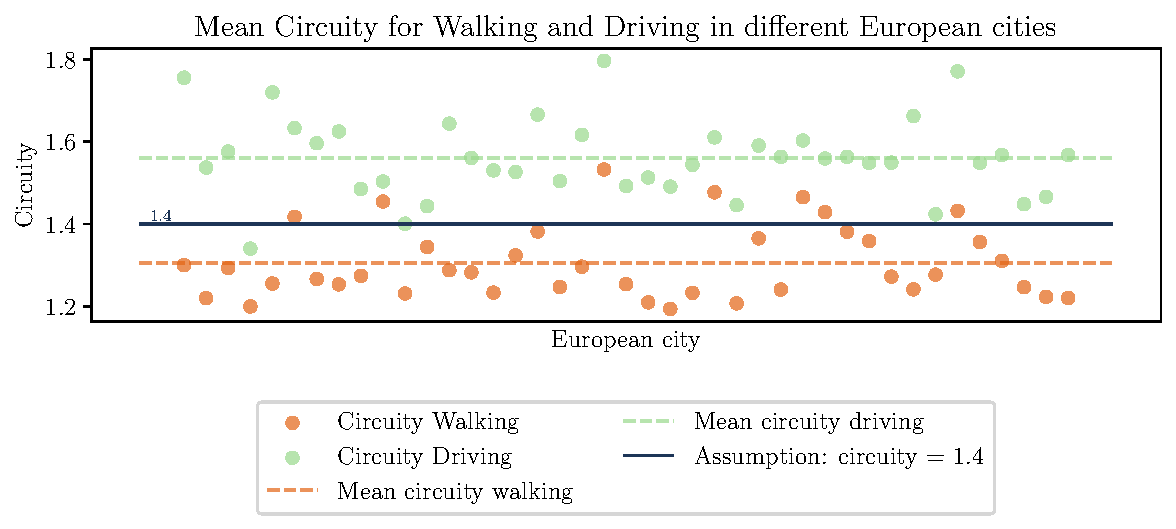
\includegraphics[width=0.8\textwidth]{graphics/mean_circuity_plot.pdf} 
    \captionsetup{labelfont={color=authorblue}, textfont={color=authorblue}}
    \caption{Circuity values for European cities published by \citep{COSTA2025106087}} \label{fig: circuity_ass}
\end{figure} 

Looking at Figure \ref{fig: circuity_ass}, the assumed circuity $\mu = 1.4$ resembles high values for driving and low ones for walking, while detouring to the closest charging site can also include walking.

To explore the impact of this assumption, we implement the reviewer's suggestion for \textbf{sensitivity analyses by varying the parameter $\mu$} according to the ranges of empirically investigated circuity. For this we test the range $\mu \in [1.0, 1.2, 1.4, 1.6, 1.8, 2.0, 2.2, 2.4]$, which we derive from report values by \citet{COSTA2025106087}. While lower circuity reflects high efficiency of transport networks, which can be present in both, rural and urban networks, high values of $\mu$ reflects less efficiency which can be also, for example, present in networks with many one-way roads. The studies on circuity are very scarce for non-urban environments. The paper by \citet{f10121147} is an exception for this and studied forest roads in mountainous areas, finding an average circuity for driving at 1.55, and maximum values at up to 2.1. 

The resulting alternative curves for the charging infrastructure expansions are displayed in Figure \ref{fig: alternative_g_SA}. The sensitivity analysis is conducted based on one densification case, i.e. the $n^{\mathrm{points~per~site}}= 10$. 

\begin{figure}[H]
    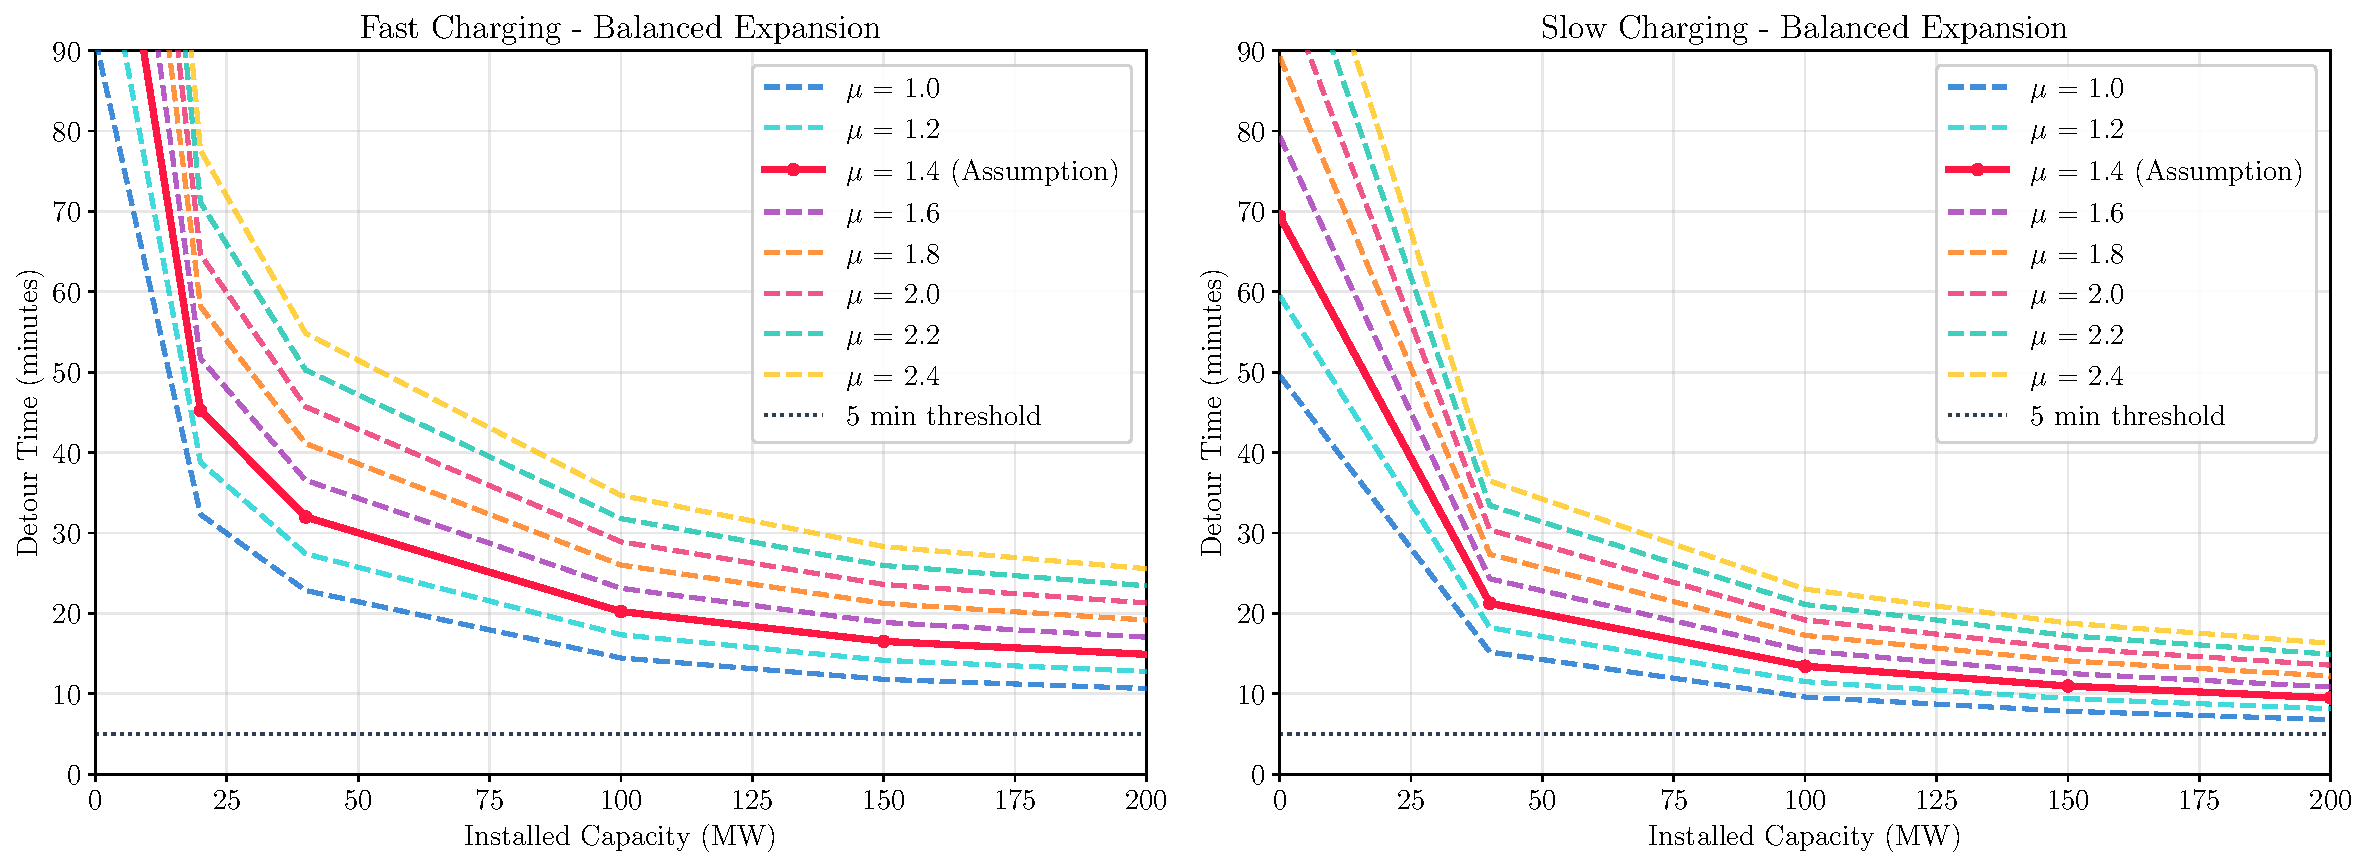
\includegraphics[width=\textwidth]{graphics/detour_time_curves_alpha_sensitivity_balanced.pdf}
    \captionsetup{labelfont={color=authorblue}, textfont={color=authorblue}}
    \caption{Tested curves for sensitivity analysis for different detour fueling time functions.} \label{fig: alternative_g_SA}
\end{figure} 

Results for the sensitivity analysis are displayed in Figure \ref{fig: SA_bev_adoption_g}, \ref{fig: SA_alpha_charged_energy} and \ref{fig: infr_comparison}.
Figure \ref{fig: SA_bev_adoption_g} displays the distribution of electrification shares over all tested $\mu$ values. The highest spread is visible in 2040 for the \textit{Medium low income} consumer group. Charging infrastructure utilization patterns by the different consumer groups are visible in Figure \ref{fig: SA_alpha_charged_energy}. Here, we observe the differences for the charging patterns for 2050. The differences among the different income classes are roughly consistent. The key observation here are:
\begin{itemize}
    \item The consumer group \textit{Very low income} mostly charges using fast charging throughout all cases. An exception for this is the scenario run $\mu = 2.0$ during which the optimal solution yielded lower fast charging usage.
    \item With increasing value of the circuity $\mu$, i.e. at lower efficiency of the transport network, work place charging is also used by consumer groups of lower income classes. 
\end{itemize}

Figure \ref{fig: infr_comparison} displays the total charging infrastructure expansion for two snapshots, 2035 and 2045. Overall, there is a consistency in the relative proportions of charging infrastructure investments by charger type. 

\textbf{Discussion:} The even-distribution assumption does not capture the spatial clustering of chargers typically observed in urban areas. Our sensitivity analysis partially addresses this: higher $\mu$ values reflect less efficient routing, which is characteristic of dense urban networks where clustering naturally occurs. Across all tested $\mu$ values, cross-income effects remain qualitatively consistent—lower-income groups continue to lag in adoption and rely more on fast charging. At higher $\mu$, we observe increased fast charging by Low income and Very low income consumers; at lower $\mu$, the average detour time is smaller (given constant public charger capacities) and charging load shifts toward public slow charging. Explicitly modeling clustered siting would require spatially explicit charger placement, which is beyond our current framework; we note this limitation in Section 5.1.2.

\begin{figure}[H]
    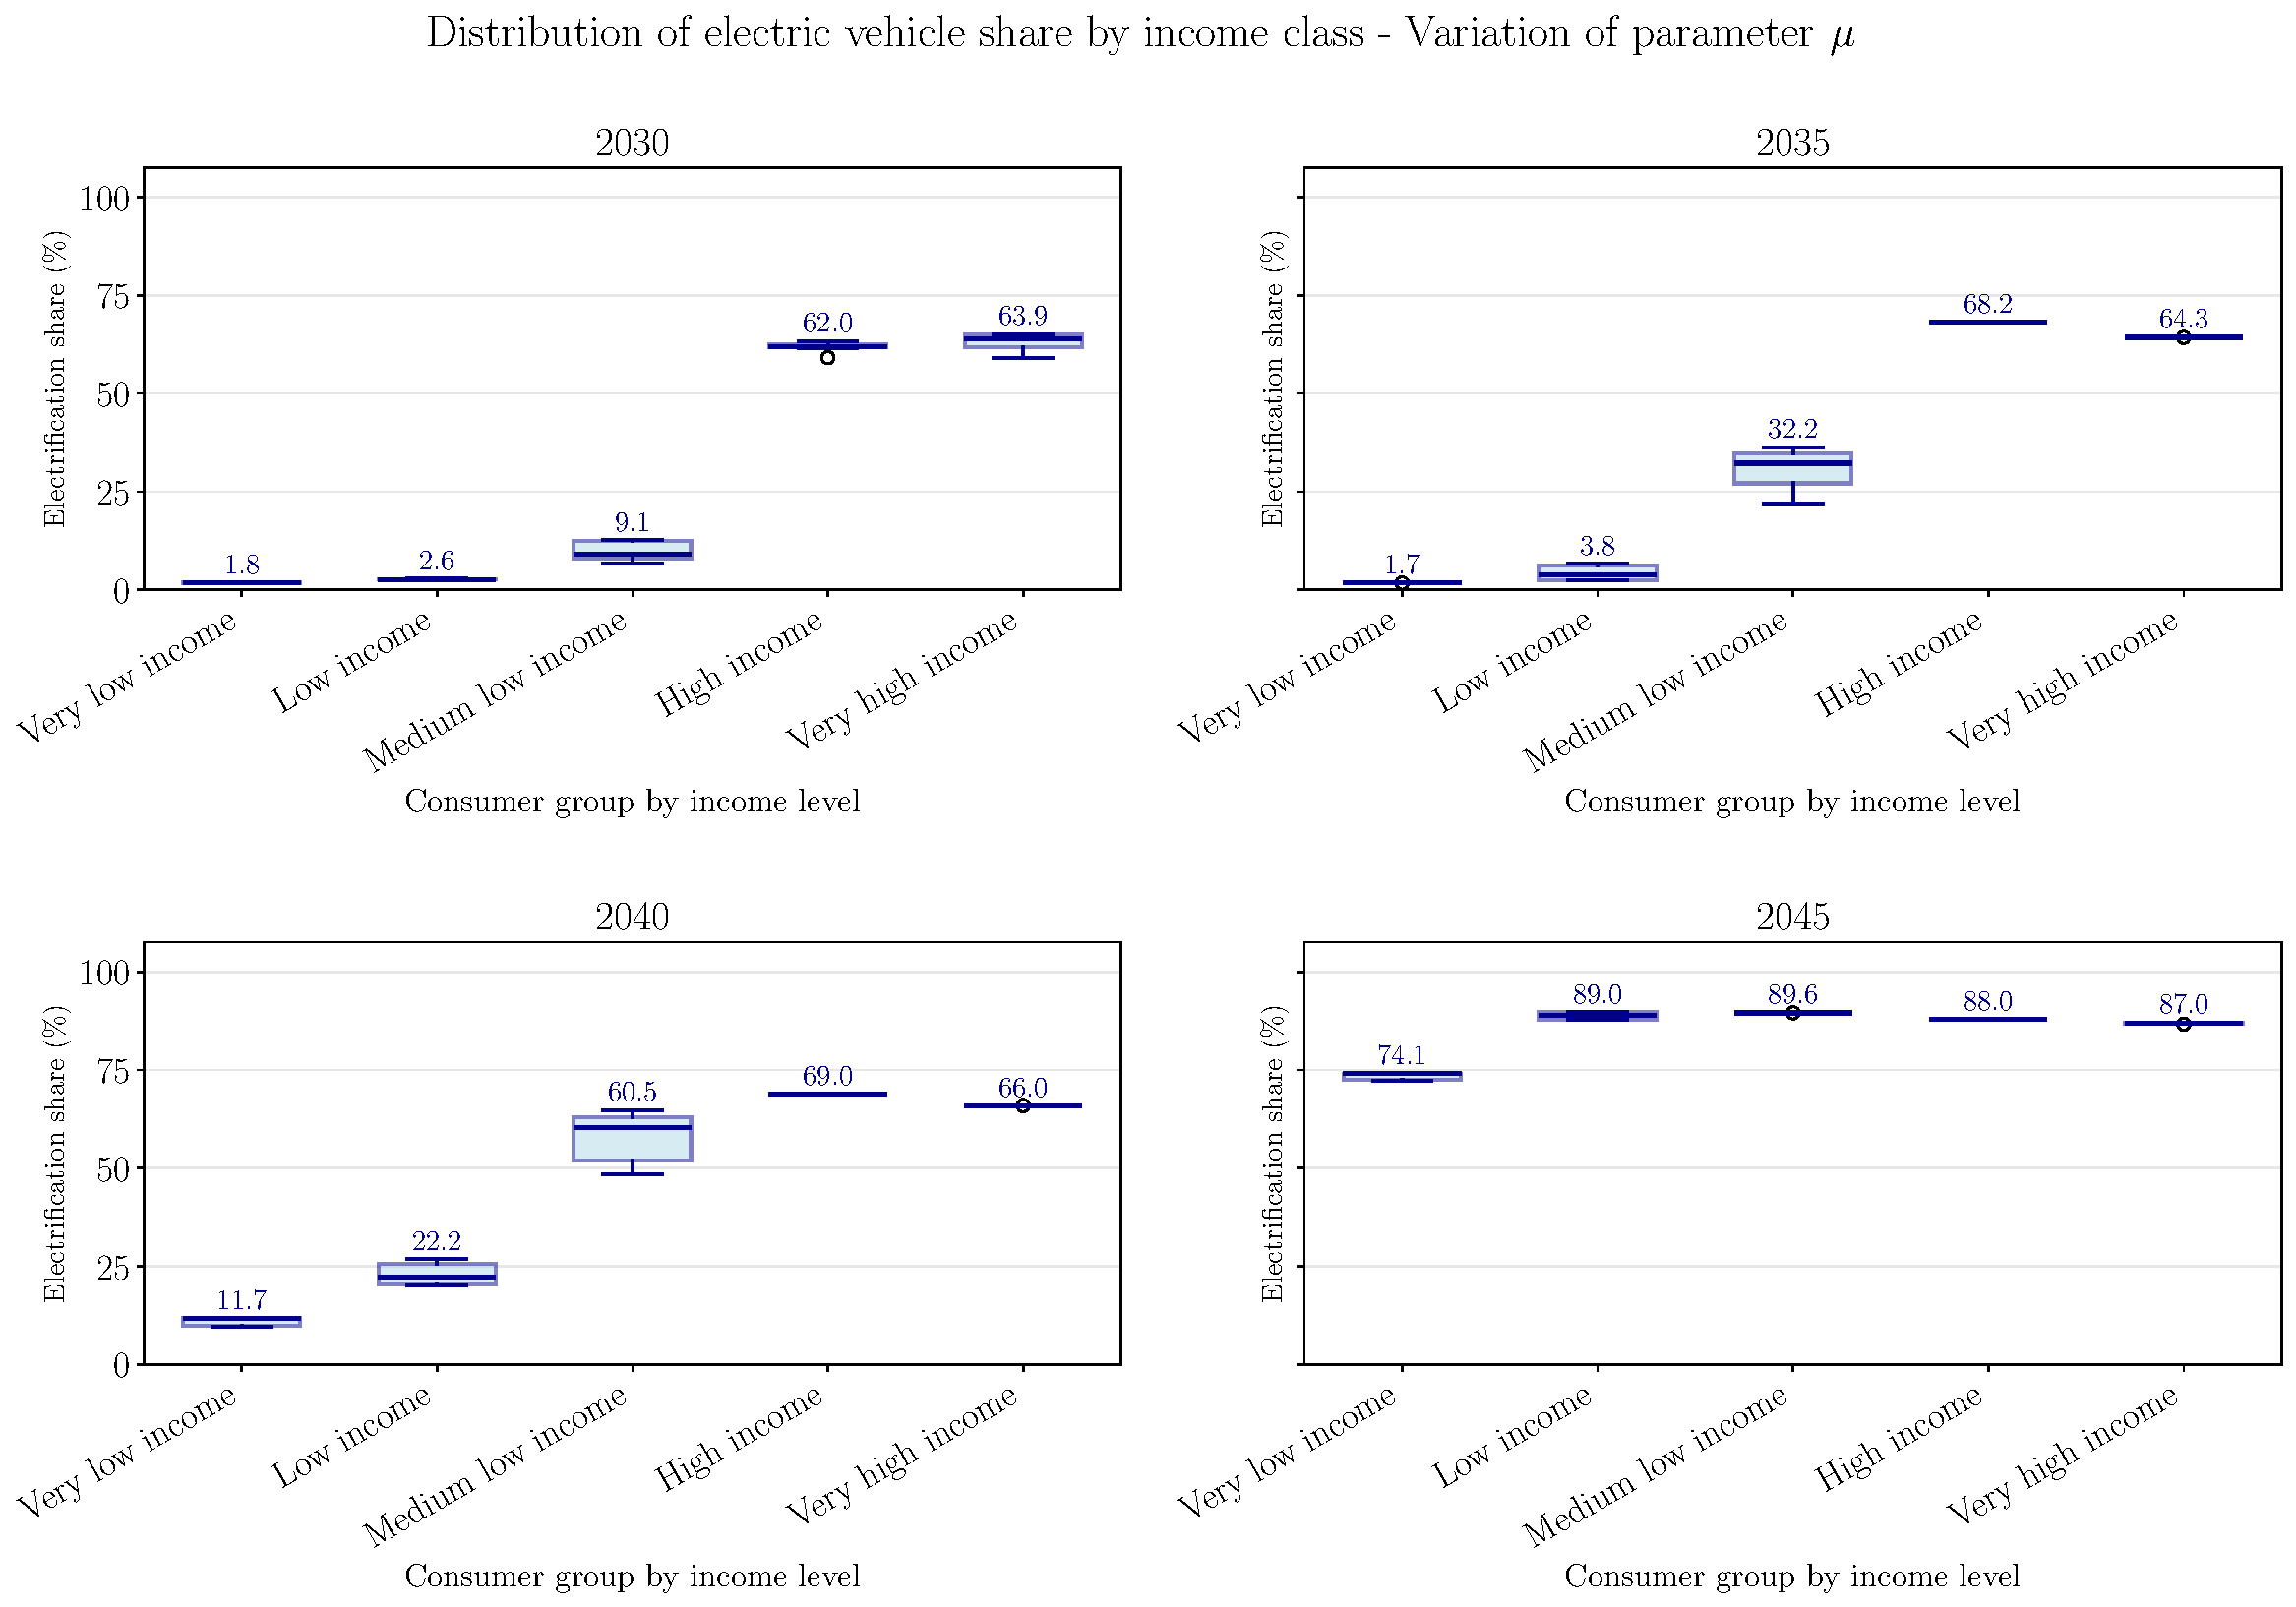
\includegraphics[width=\textwidth]{graphics/SA_alpha_boxplot_electric_vehicles_by_income_mu.pdf} 
        \captionsetup{labelfont={color=authorblue}, textfont={color=authorblue}}

    \caption{Distribution of the development of the electrification of passenger car fleet owned by consumer groups of different income levels for different parameterization of circuity $\mu$.} \label{fig: SA_bev_adoption_g}
\end{figure} 


\begin{figure}[H]
    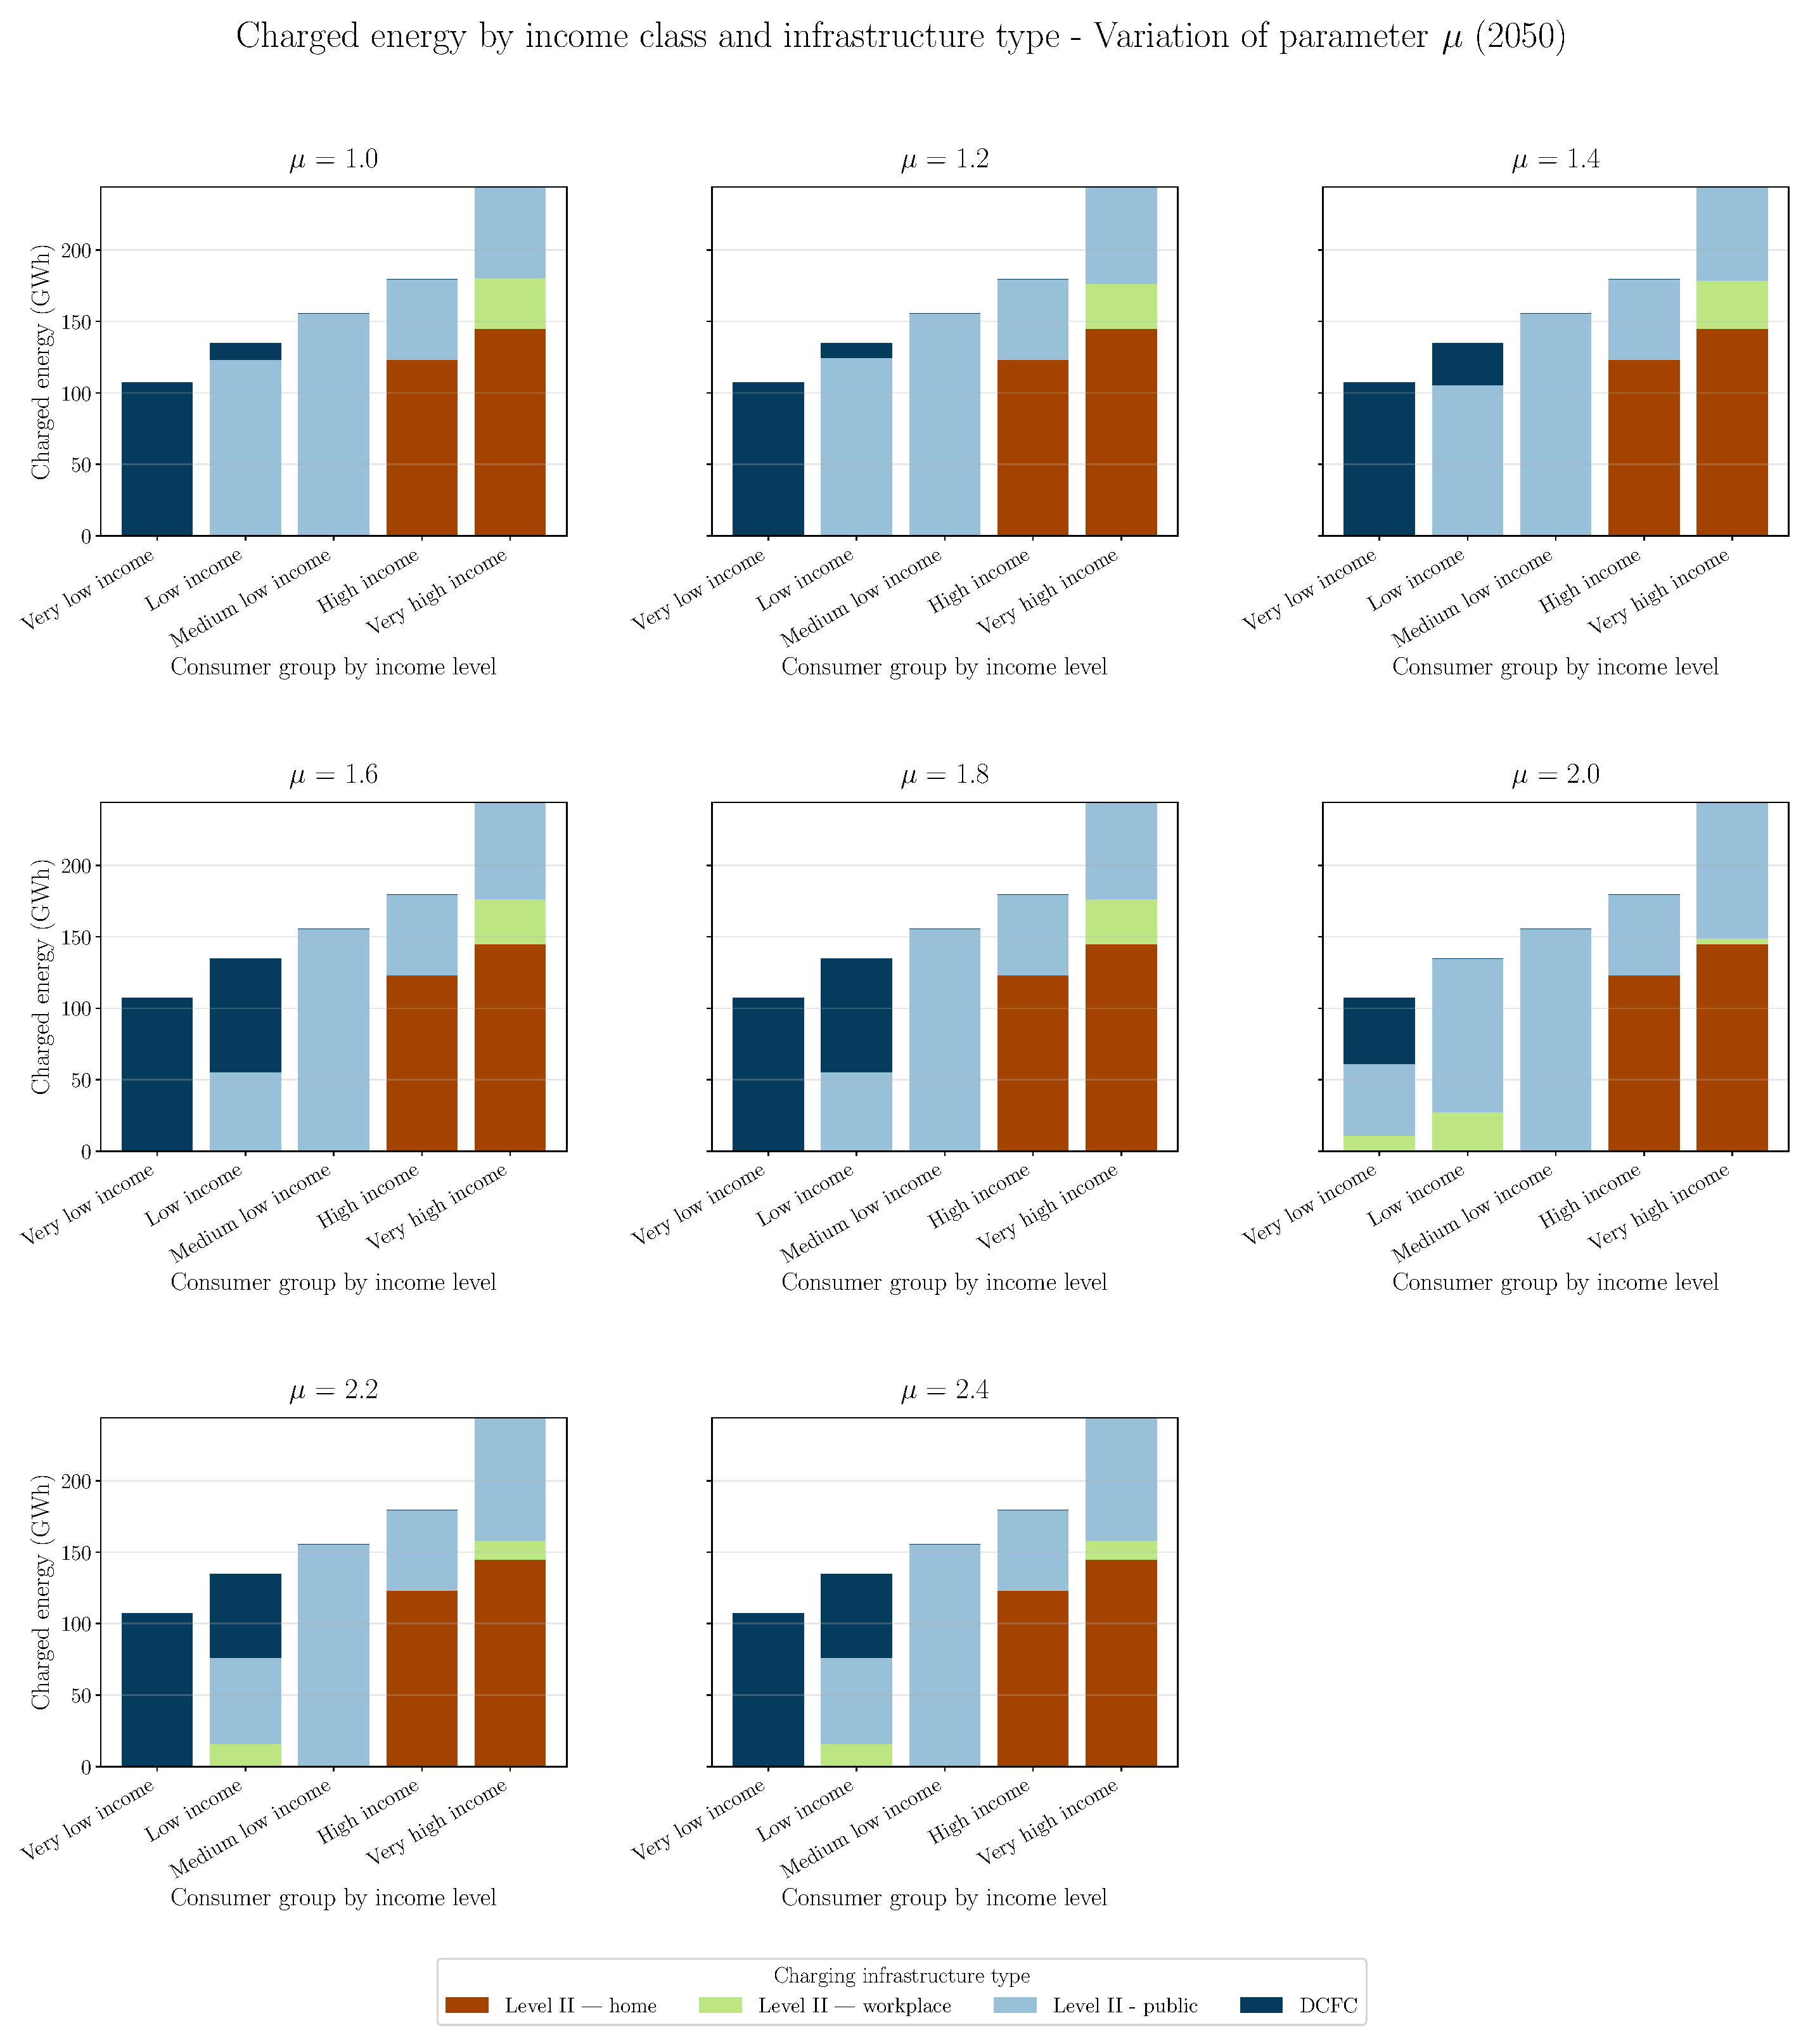
\includegraphics[width=\textwidth]{graphics/SA_alpha_charged_energy_by_income_infrastructure.pdf}
    \captionsetup{labelfont={color=authorblue}, textfont={color=authorblue}}

    \caption{Charger utilization 2050 under different parameterizations of circuity $\mu$.} \label{fig: SA_alpha_charged_energy}
\end{figure} 


\begin{figure}[H]
    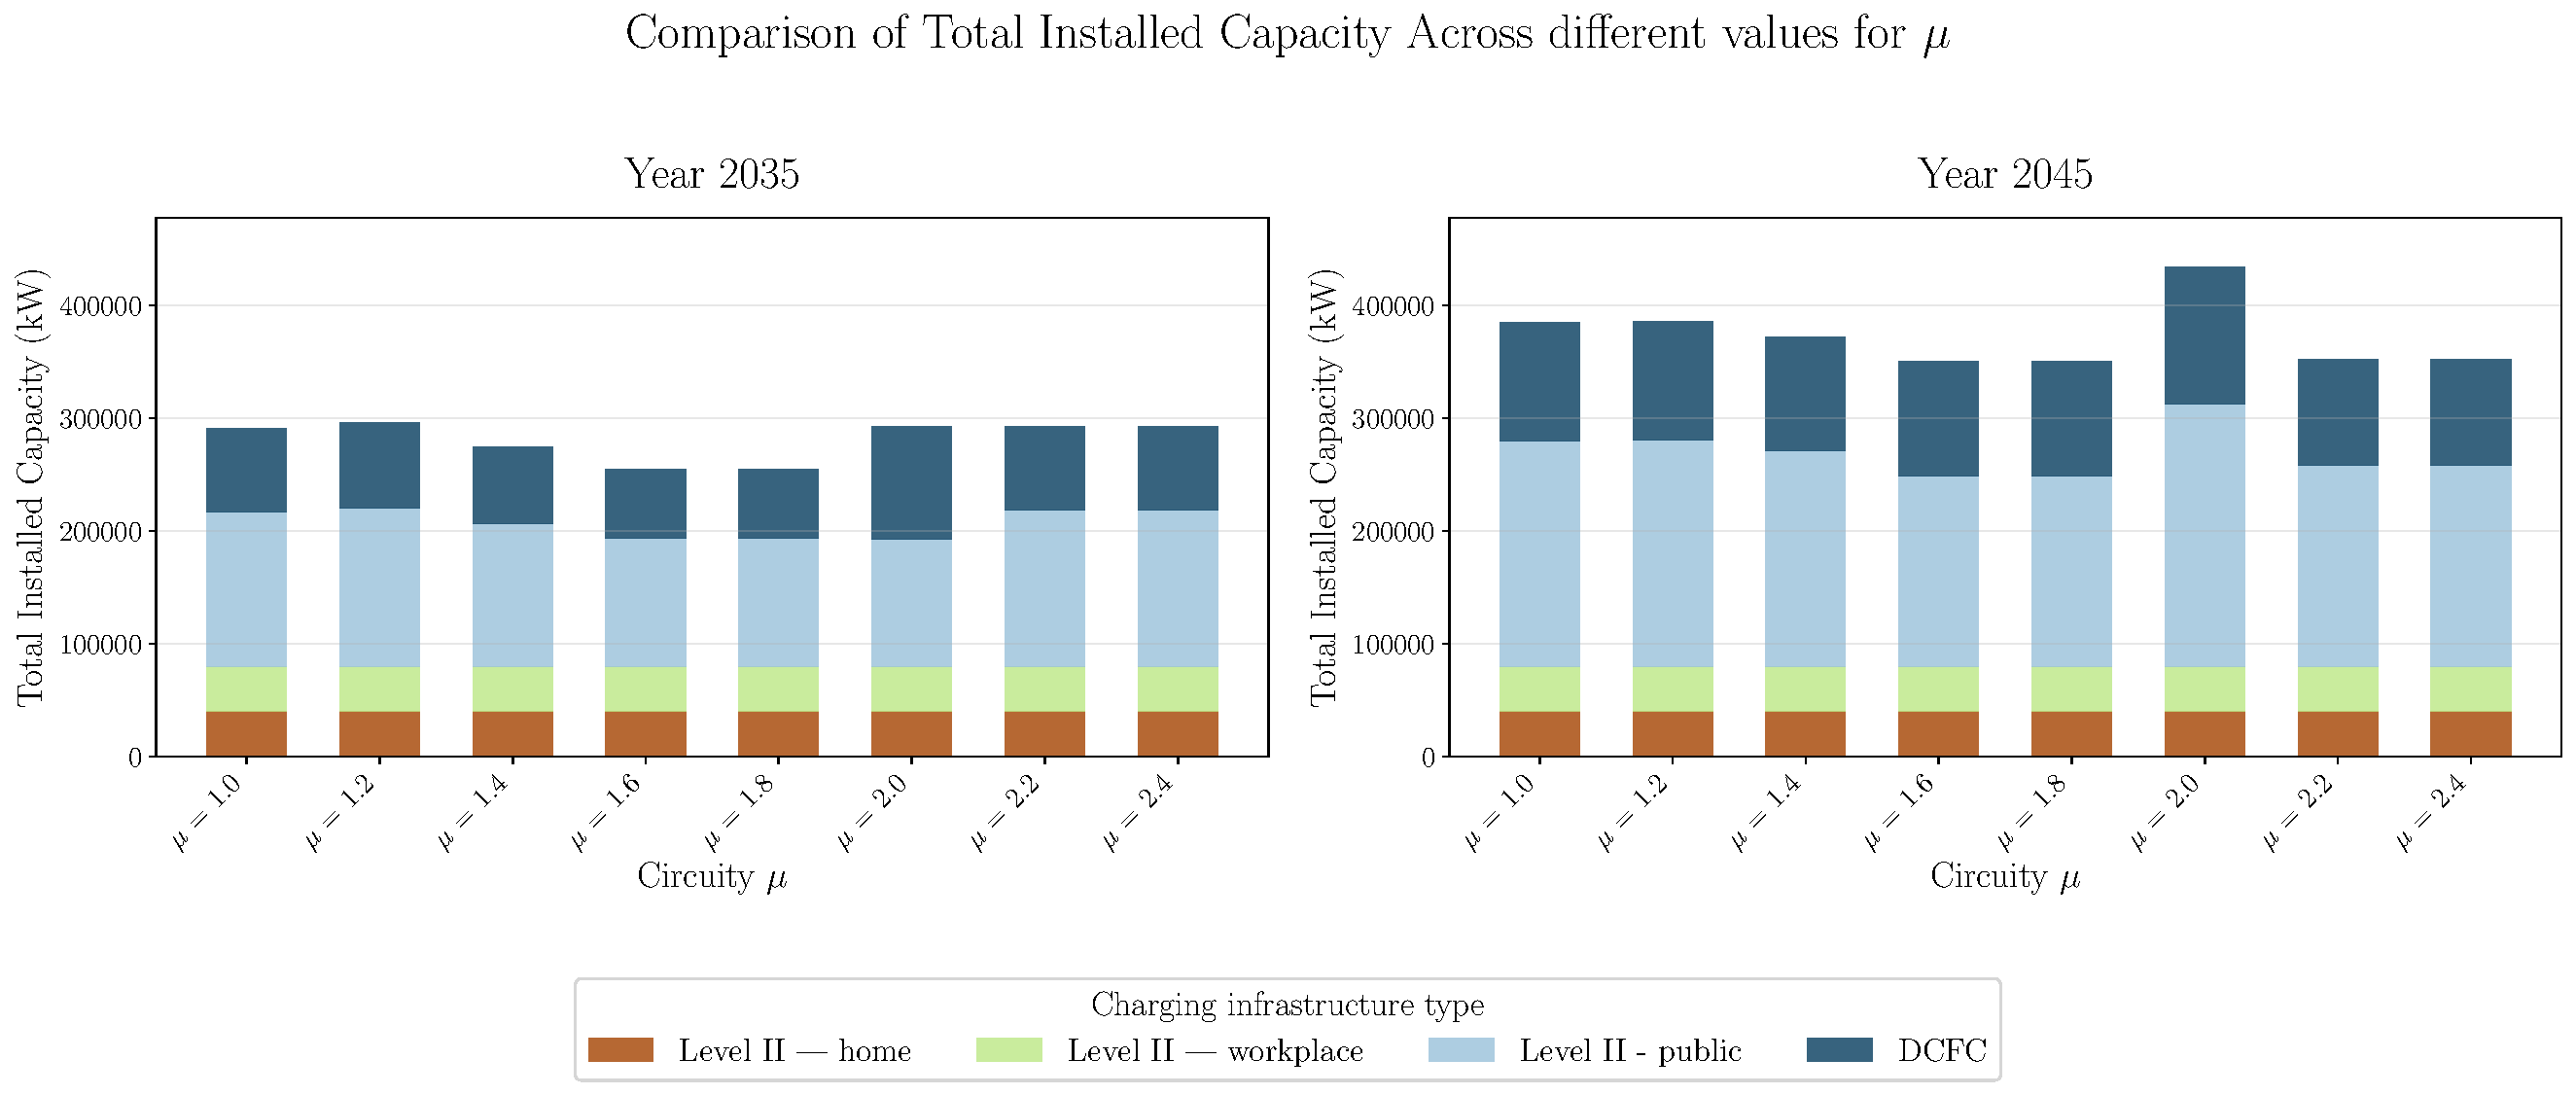
\includegraphics[width=\textwidth]{graphics/SA_alpha_capacity_comparison_2035_2045.pdf} 
    \captionsetup{labelfont={color=authorblue}, textfont={color=authorblue}}
    \caption{Comparison for total installed charging infrastructure for different value of circuity $\mu$.} \label{fig: infr_comparison}
\end{figure} 

We have now included the description of this sensitivity analysis, the description and discussion of results in the \textbf{appendix of the manuscript (see Section B.1)}. Further, we have \textbf{refined the description} of the detour fueling time for better understanding (see Section 3.4).



%We acknowledge that there is a wide range of literature that is particularly dedicated to the topics of facility allocation in regard to average distance minimization and studying the differences between empirical distances. We leverage this strand of research in designing the detour time function. The average circuity of the road network, i.e., the ratio between the Euclidean distance and the distance in the road network, is estimated to be 1.4 in our analysis. The following figure displays measured values for different European cities which are drawn from a recent study by [Costa et al., 2024] together with the assumed value for us. The Basque country has 71\% of population in rural areas [EUSTAT database]. We draw from city-based circuity data due to the lack of empirical data for the Basque country and the lack of empirical studies on rural areas. A similar study, comparing road network circuity across multiple countries worldwide, was published in 2002 [Ballou et al., 2002]. We also include its value in this graphic, although it is likely outdated.

%\hl{*hier füge ich noch eine Graphik ein mit einem Strahl von verschiedenen werten für die Circuity aus der Literatur versus die Annahme von 1.4; *}
%To compensate for this unknown factor in the circuit value, we design two scenarios for the sensitivity analysis: … and we test the these for the $n^{points per site = 10}$. 
% \textit{In the results, we look at BEV adoption and utilization results, as well as charging patterns by income class}



\color{reviewergrey}
\subsubsection*{2. Value of Time (VoT) and income-class parameter choices need local calibration and sensitivity\\
\textbf{Issue:} VoT for income classes is borrowed from a Danish study and scaled by purchasing power. Spain/Basque Country VoT may differ meaningfully. Since VoT drives how income groups trade off detour/charging time vs other costs, results (e.g., why low-income tolerate long fast-charging detours) hinge on VoT. \\ \\
\textbf{Required:}\begin{itemize}
    \item Justify VoT choice with local evidence (citations, national surveys, or sensitivity bounds).
    \item Add sensitivity runs where VoT for each quintile is varied $+ - $30\% (or a plausible band) and show impact on BEV adoption and charging utilization by income. If surveys for Spain exist, use them to support parameter choices.
\end{itemize}
}{}
\color{authorblue}
 \noindent \textcolor{authorblue}{\textbf{Author's response:}}  Thank you for highlighting this limitation. This issue has been highlighted also by the other reviewers. We agree that the transfer of the VoT data from the Danish study to the Basque country is a strong assumption. In the following we describe the \textbf{justification of the VoT parameterization} and \textit{the results of sensitivity analysis for different VoT scenarios}. \\

\textbf{Justification of VoT choice:} Due to the lack of region-specific data for the Value of time (VoT) for different consumer groups, we have drawn from data for Denmark based on a published study by \citet{TATTINI2018265}. The reasoning behind the usage of the data by \citet{TATTINI2018265} is twofold: First, the availability of a range of values that specifically describe different levels of income. Second, the study by \citet{TATTINI2018265} applied these values in a methodologically similar manner, which also informs the foundation of our approach. \\ 
Concerning the scaling that is mentioned in this comment, we base the usage of the Purchase Power Parity measure for the conversion of the values between the countries based on the publication by \citet{WARDMAN201693}. The authors explicitly address the main determinants of the VoT by comparing studies from different countries and applying exploratory analysis to identify relevant parameters that lead to the country/study differences. They identify the cost of living, type of trip and mode type to be the most relevant influencing parameters. We are, therefore, confident that our assumed VoT values by income class reflect the VoT values of Spain.\\

\textbf{Sensitivity analysis:} In accordance with the recommendation, we conducted additional sensitivity analysis to assess the potential impact of the parameterization of the VoT values. In the design of the sensitivity analysis, we tackle two aspects: Different absolute values and relative differences between the income classes. The following two figures display the tested VoT scenarios:

\begin{figure}[H]
    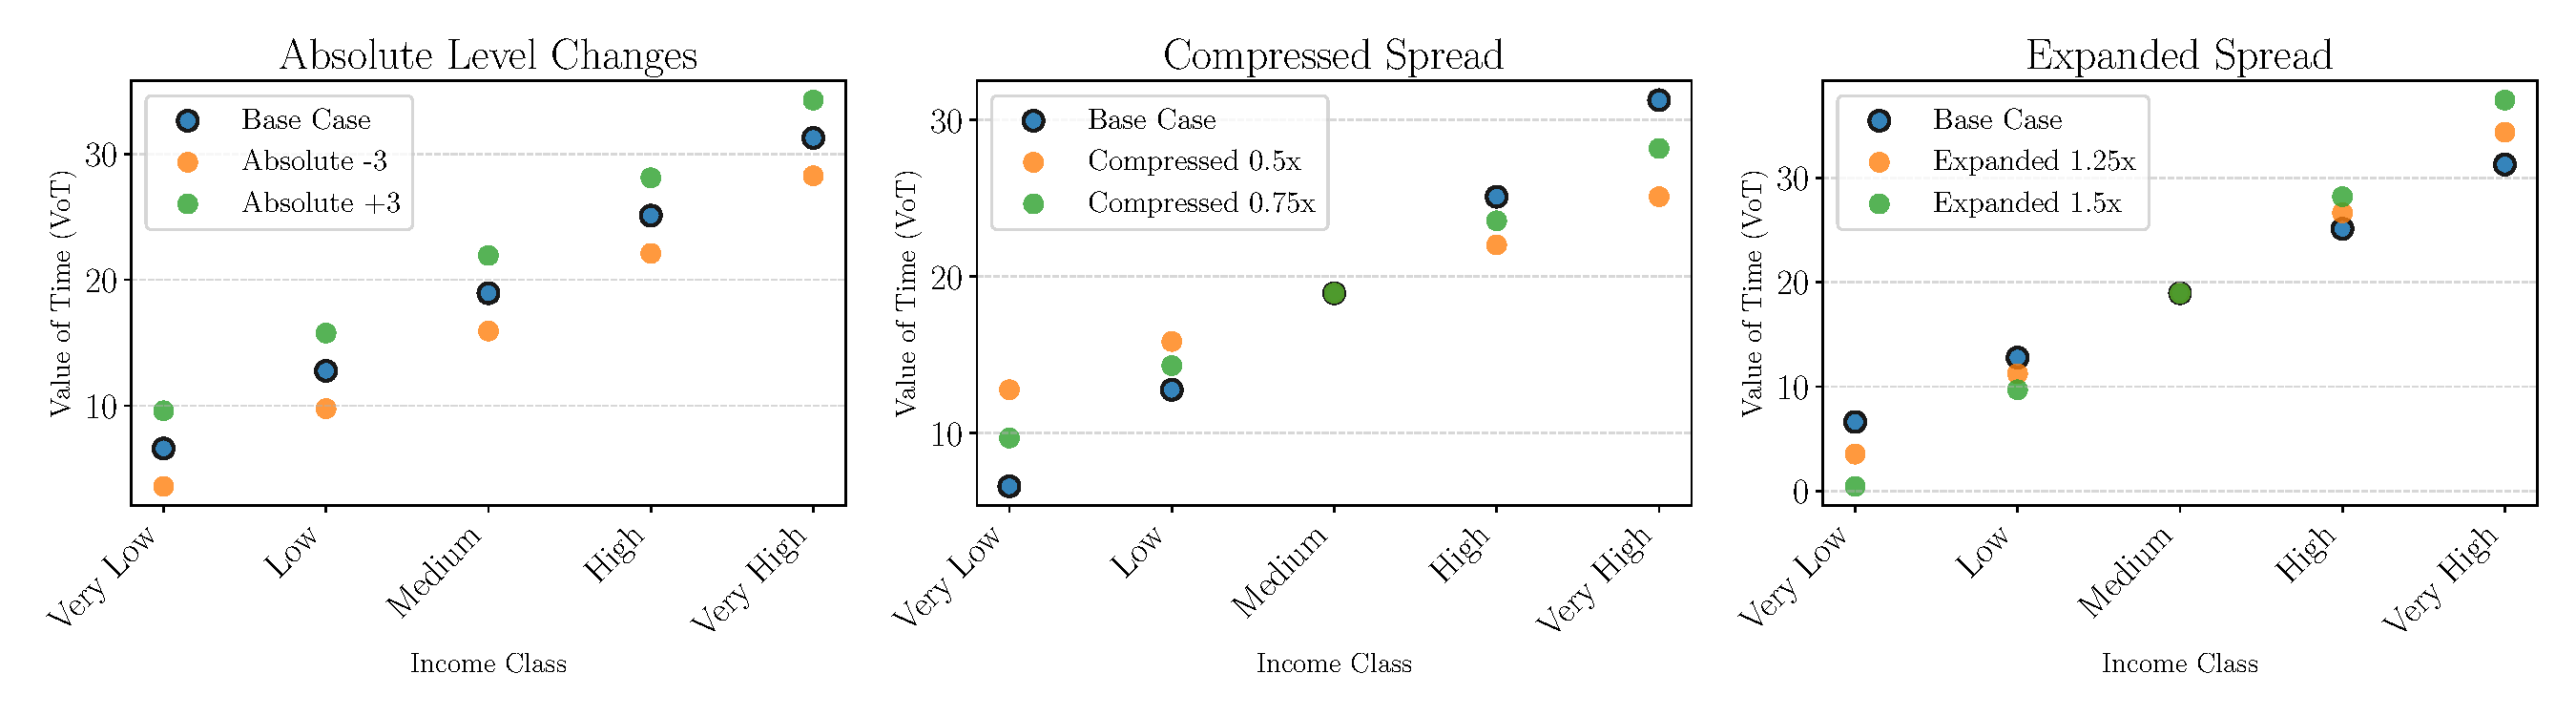
\includegraphics[width=\textwidth]{graphics/sensitivity_analysis_vot.pdf} 
        \captionsetup{labelfont={color=authorblue}, textfont={color=authorblue}}

    \caption{The \textit{Base Case} displays the assumed VoT values for the Basque country. \textit{Left:} VoT values for absolute increase and decrease of the value of time. \textit{Center:} Two cases of smaller relative changes between the VoT per income class. \textit{Right:} Higher relative changes between the VoT per income class.} \label{fig: VoT_tesing}
\end{figure} 

The tested shifts of absolute levels are $\pm 3$ which equal approximately absolute differences between the VoT values between inter-city vs. urban car trips in Spain \citep{WARDMAN201693}. As the \textit{Base Case} for this sensitivity analysis we use the densification scenario of $n^{\mathrm{points per site}} = 10$.

Figure \ref{fig: VOT_bevs_10} displays the distribution of electrification shares by the consumer groups for years 2030, 2035, 2040 and 2045. Overall, no significant outliers are shown. The highest impact of the VoT parameter is visible for the consumer group \textit{Medium low income}. This particularly becomes visible for the years 2035 and 2040, where the spread is up to around 45\%. The extreme values here are particularly given by \textit{Expanded 1.25x} and \textit{Expanded 1.5x}, and \textit{Compressed 0.5x} and  \textit{Compressed 0.75x}. The average VoT of these VoT scenarios are the same. Therefore, there is a particular sensitivity to the relative differences between the income-class specific VoT parameters in the adoption of BEVs. 

\begin{figure}[H]
    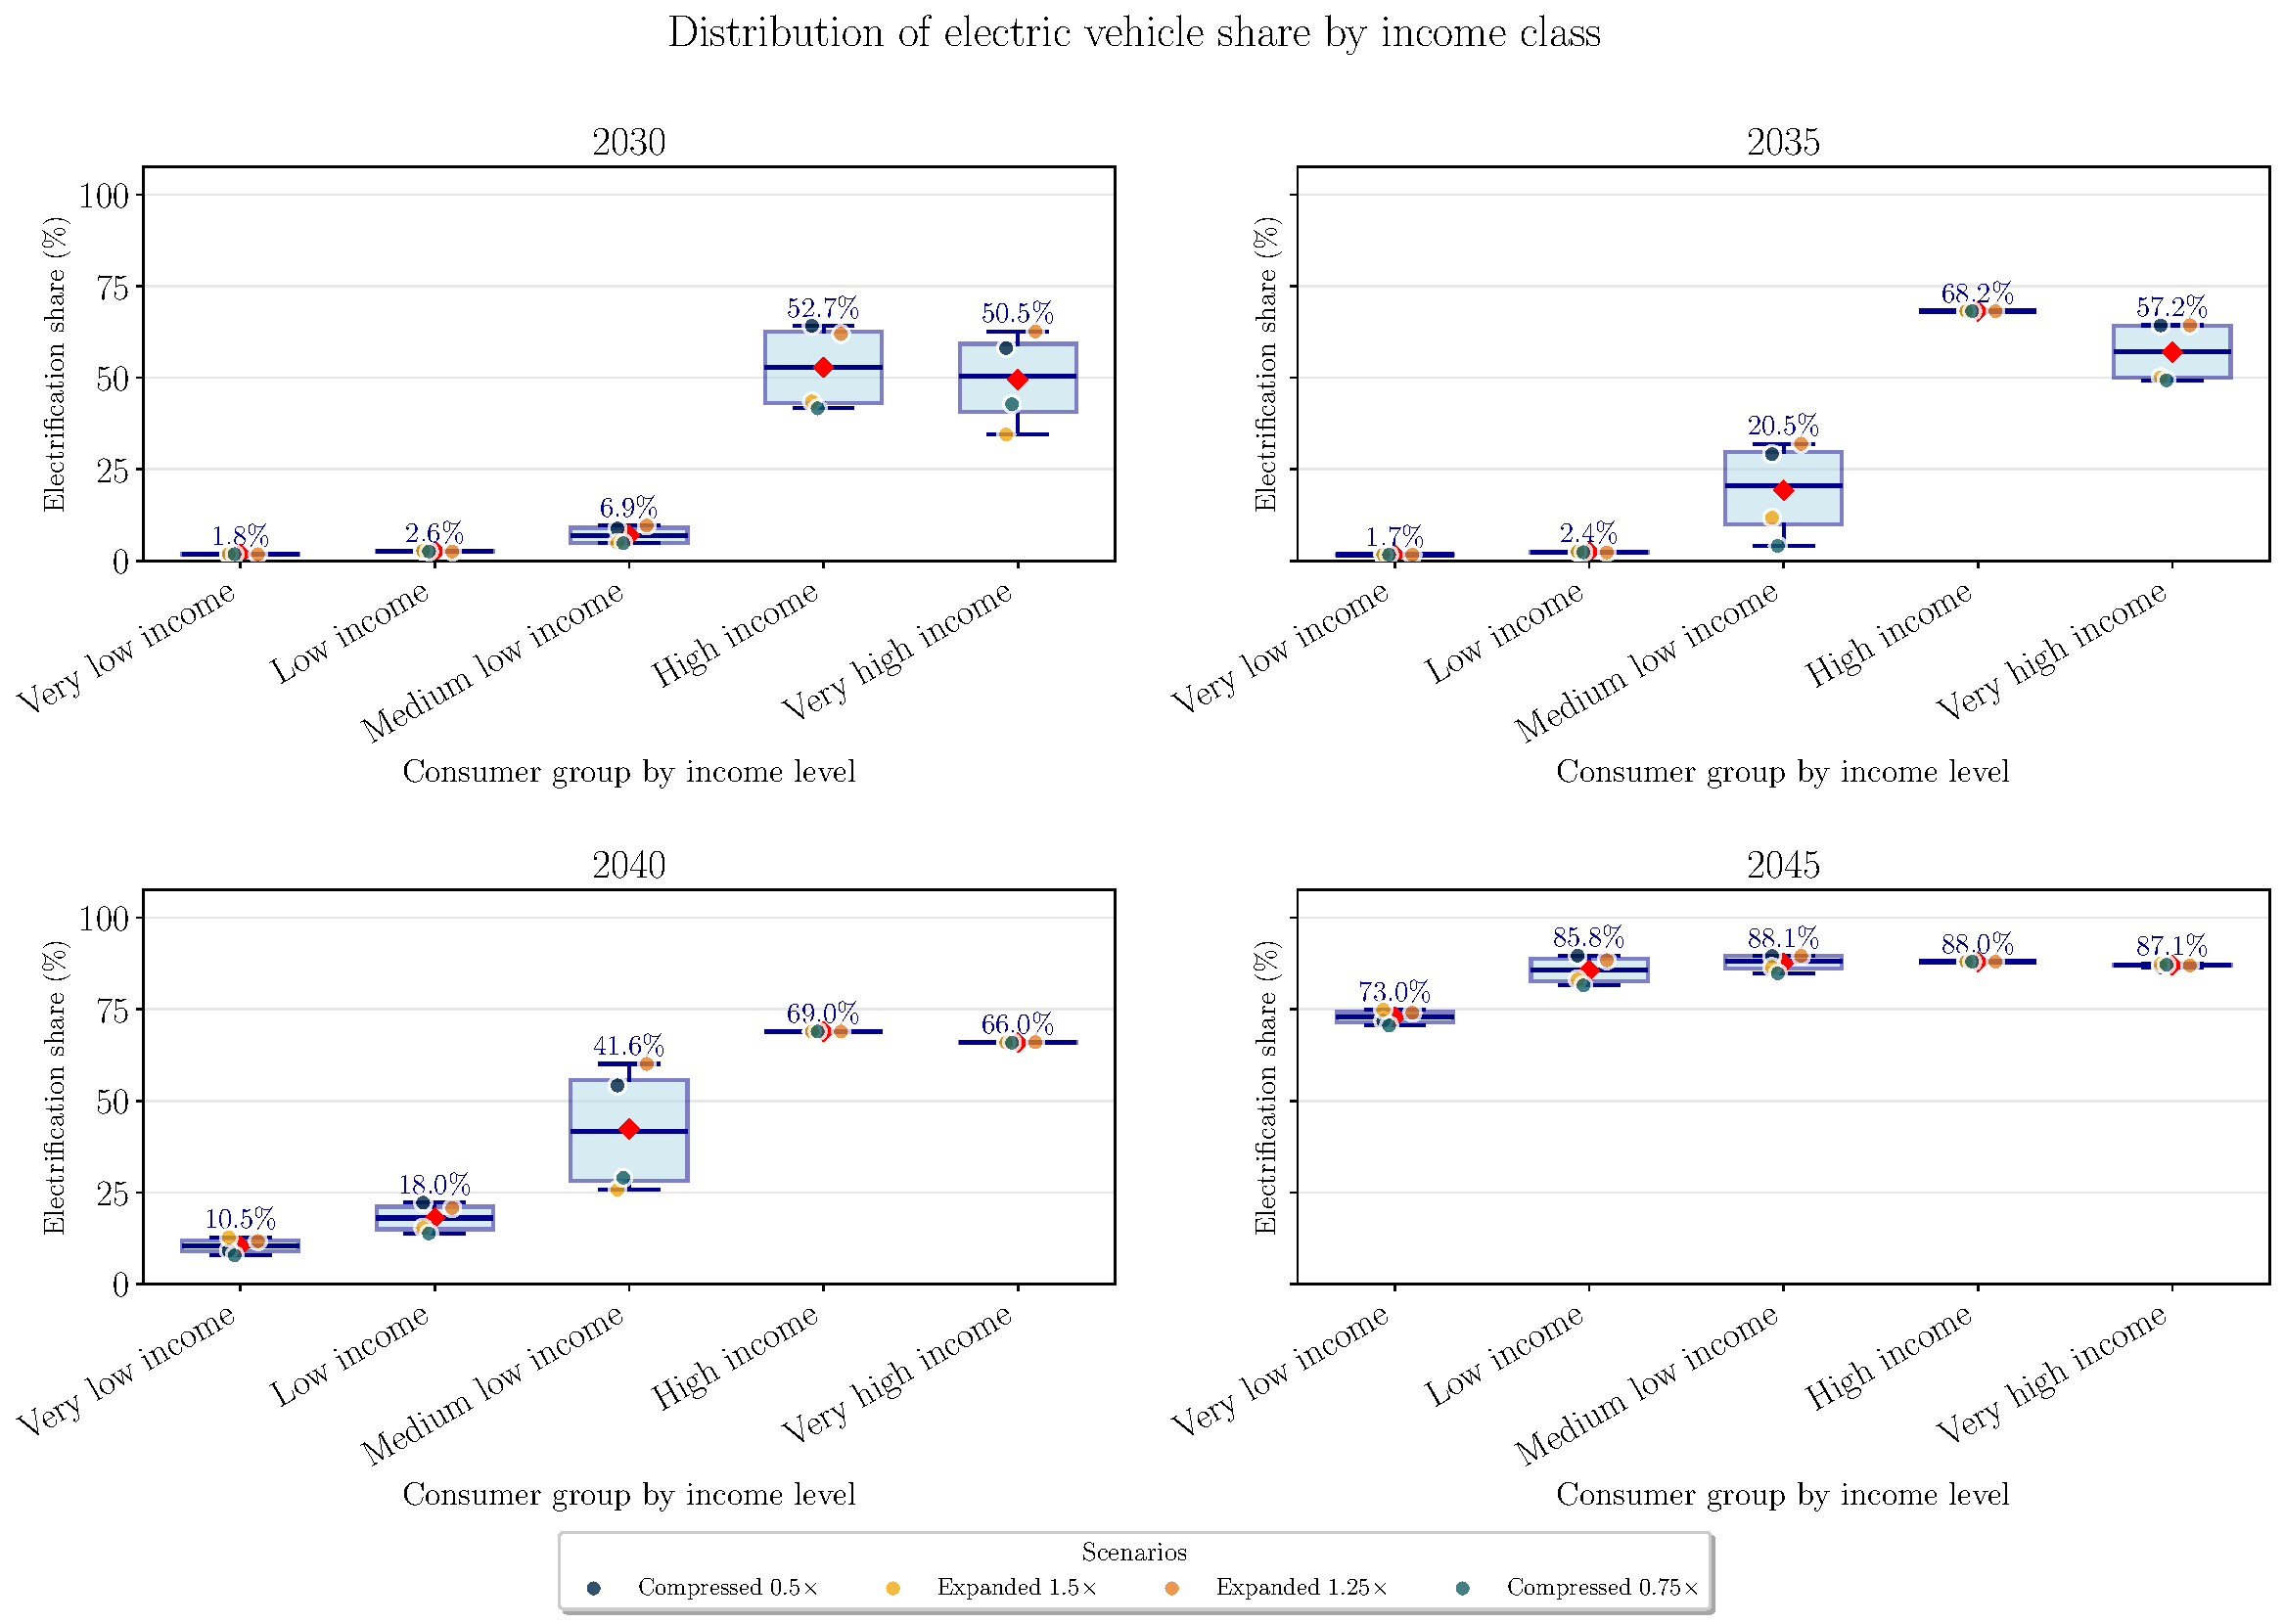
\includegraphics[width=\textwidth]{graphics/SA_boxplot_electric_vehicles_by_income.pdf} 
        \captionsetup{labelfont={color=authorblue}, textfont={color=authorblue}}

    \caption{Distribution of the development of electrification of passenger car fleet owned by consumer groups of different income levels observed during sensitivity analysis of different VoT parameterization.} \label{fig: VOT_bevs_10}
\end{figure} 

To address the reviewer’s suggestion regarding charging patterns, we next examine the differences in charged energy across charger types (see Figure \ref{fig: VOT_charging_pat_3}). We show here at a snapshot for 2050 showing the usage patterns by the 100\% electrified fleet for a selection of four different VoT parameterizations. While there are no significant changes for consumer groups \textit{Very high income}, \textit{High income} and \textit{Medium low income}, the amount of fast charging capacity being used by the \textit{Very low income} and \textit{Low income} varies significantly between the VoT settings.

In Figure \ref{fig: VoT_fastcharg_ut_3}, we take a closer look at the usage of fast charging capacities by  \textit{Very low income} and \textit{Low income} consumer groups. In the cases where these groups have higher VoT, i.e. the VoT scenarios of \textit{Compressed 0.5x},  \textit{Compressed 0.75x} and \textit{Absolute +3}, the amount of fast charging is zero for the \textit{Low income} class.

\begin{figure}[H]
    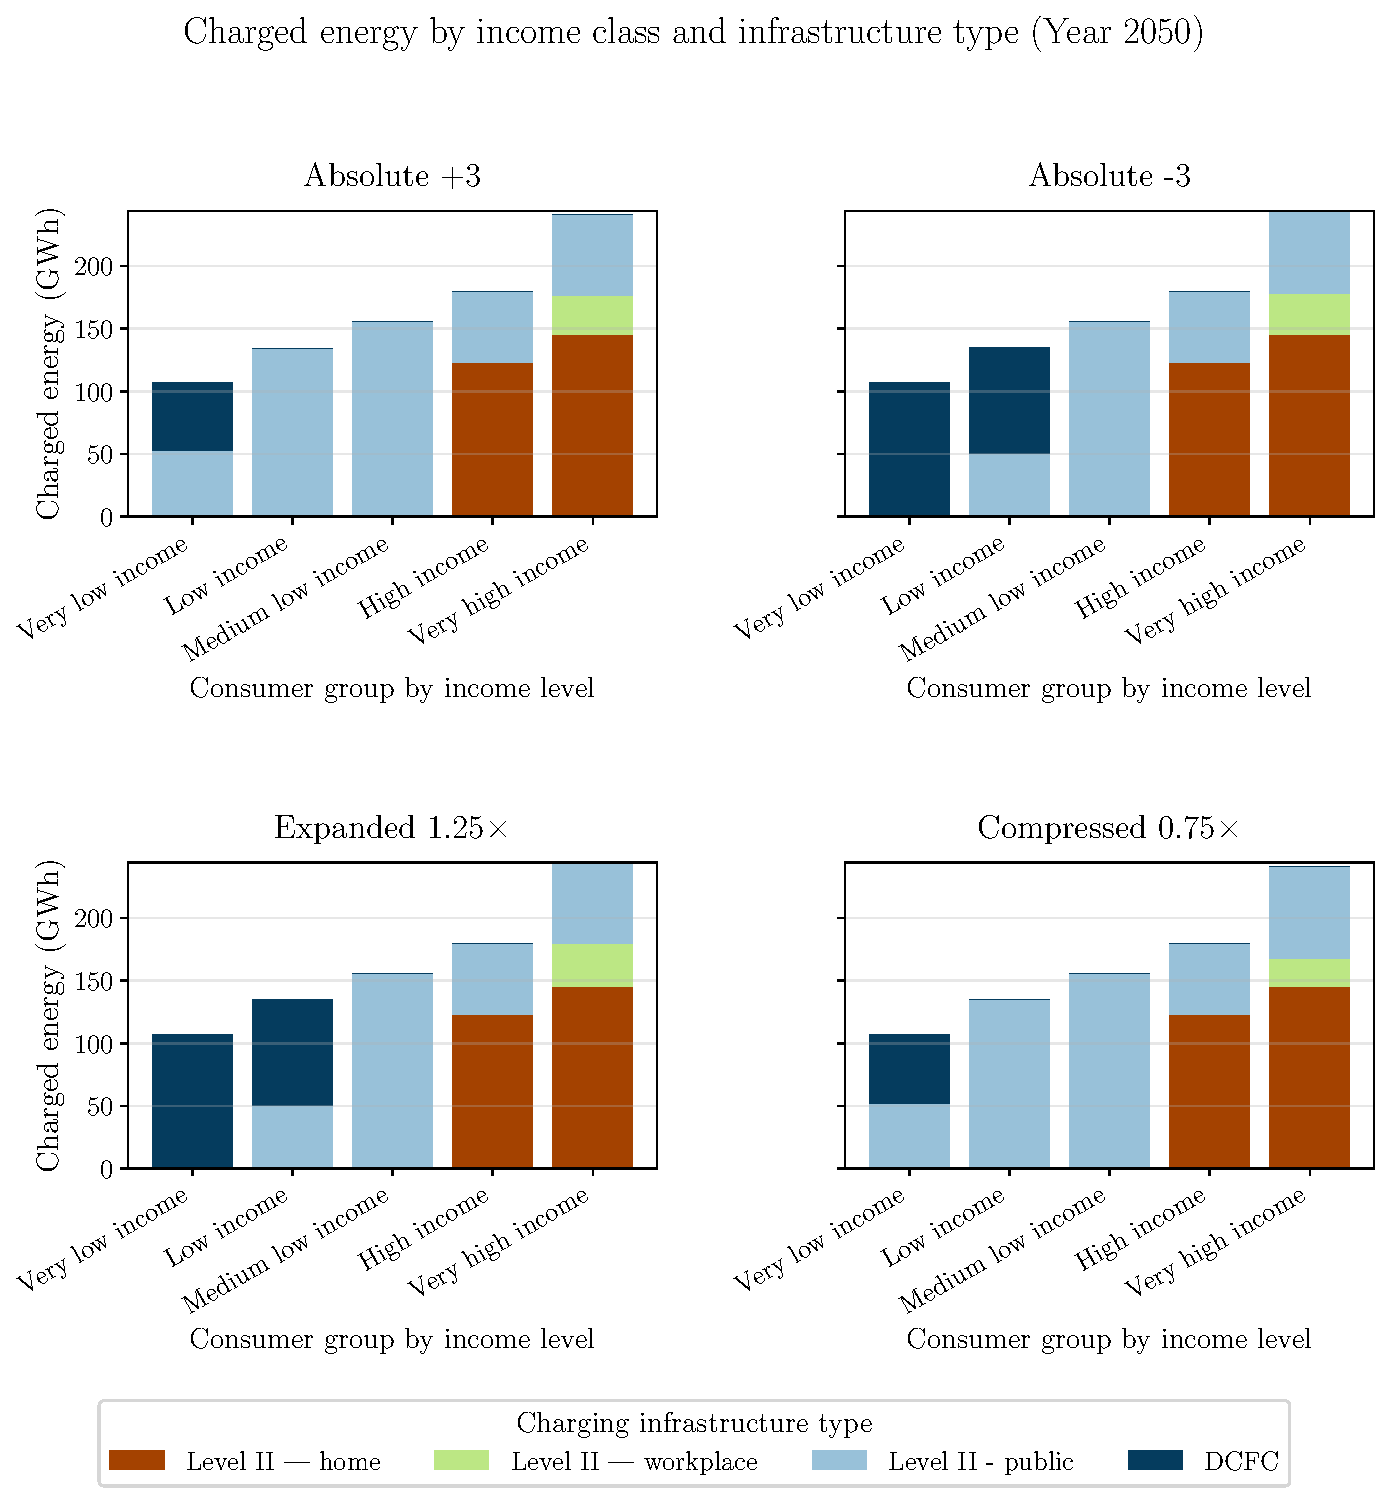
\includegraphics[width=0.7\textwidth]{graphics/SA_charged_energy_by_income_infrastructure.pdf} 
        \captionsetup{labelfont={color=authorblue}, textfont={color=authorblue}}

    \caption{Charged energy by charger type in 2050 for different VoT scenarios.} \label{fig: VOT_charging_pat_3}
\end{figure} 

\begin{figure}[H]
    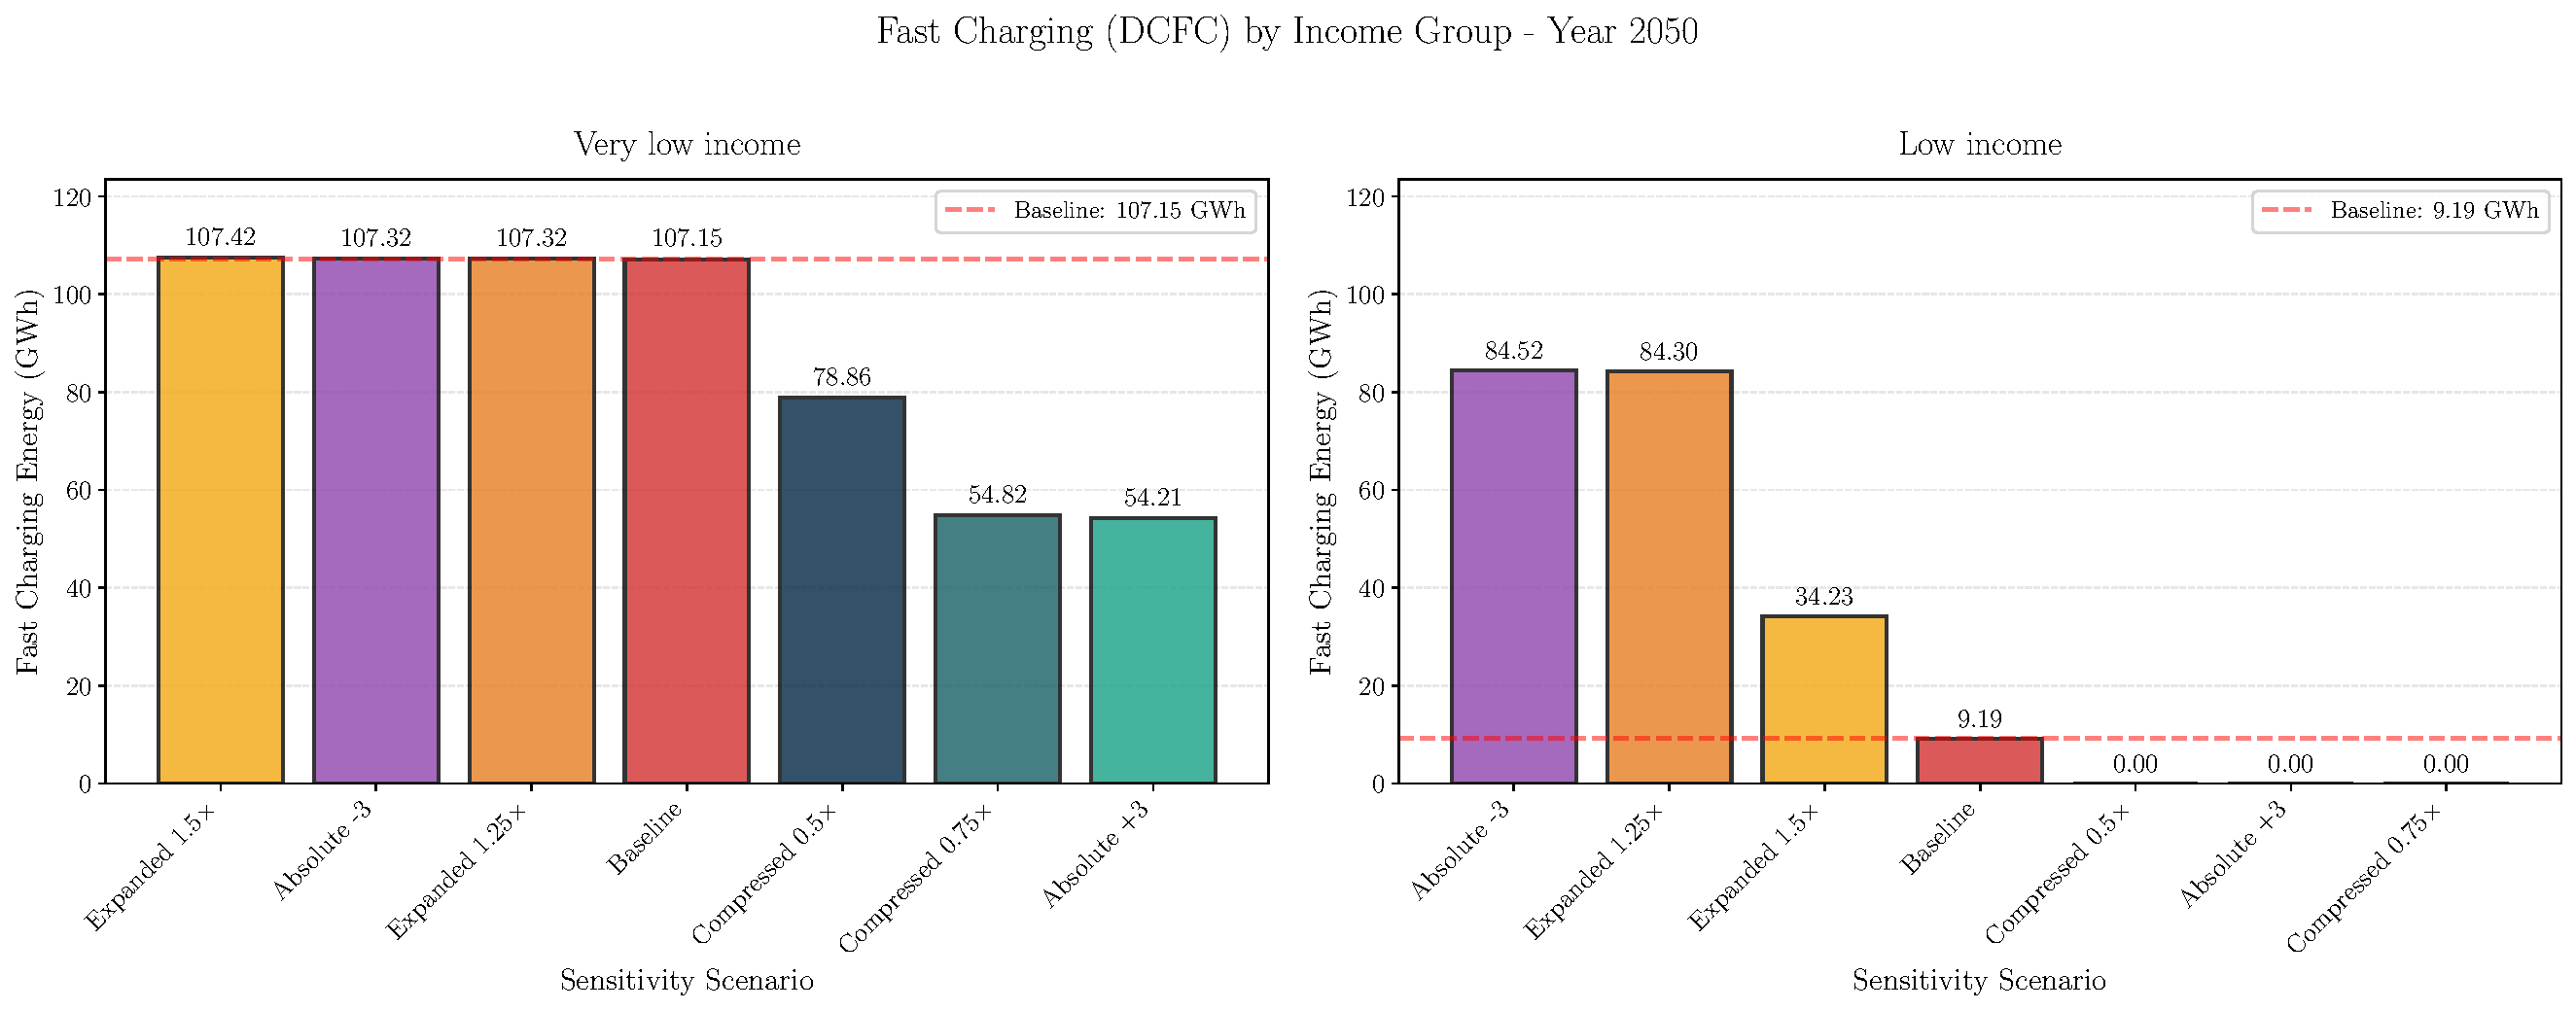
\includegraphics[width=0.9\textwidth]{graphics/SA_fast_charging_low_income_comparison.pdf} 
        \captionsetup{labelfont={color=authorblue}, textfont={color=authorblue}}

    \caption{Charged energy at fast chargers in 2050 for different VoT scenarios for consumer groups \textit{Very low income} (left) and \textit{Low income} (right).} \label{fig: VoT_fastcharg_ut_3}
\end{figure} 

This observation is coherent with observations presented in the \textit{Results} section, in particular, Section 4.1. where we show differences of fast charger utilization through variation in levels of service induced by charging infrastructure densification. There, as well as in these VoT scenarios, we observe how the term $\mathrm{VoT} \times \mathrm{level~of~service}$ influences charger-type utilization across income groups.    

To provide a better understanding of the setting of the VoT parameter to the reader, we have now included this sensitivity analysis in the appendix of the manuscript (see Section B.2.).
\color{reviewergrey}
\subsubsection*{3. Home charging treatment and behavioral preference \\
\textbf{Issue:} Model does not expand home charging because of budget constraints and low maximum utilization assumptions; yet empirical evidence and other studies show home charging remains central and preferred where possible. The current level-of-service formulation does not capture preference for residential convenience, and results show unexpected low expansion of home chargers.\\\\
\textbf{Required}:\\
\begin{itemize}
    \item Add an explicit utility/penalty or preference for home charging (or a parameter that increases its effective VoT benefit) so the model can represent convenience value beyond utilisation.
    \item Alternatively include scenario(s) where home-charging expansion is exogenously allowed to reach higher ceilings (consistent with observed homeowner shares) and show results.
\end{itemize}
}
\color{authorblue}
\noindent \textcolor{authorblue}{\textbf{Author's response:}}  Thank you for highlighting this limitation of the methodology. This limitation stems from the techno-economic modeling which optimizes charging infrastructure capacities based on the utilization efficiency and cost-optimality. The convenience of home charging is reflected in the zero detour time associated with its use. However, due to low utilization rates and monetary budget constraints, the model does not select home charging expansion as part of the cost-optimal solution. We acknowledge this limitation in the “Limitations” section (Section 5.2.1.). 

In response to the reviewer's comment, we explicitly include the requirement for the extension of the level-of-service feature to capture this type of convenience beyond detouring time as \textbf{“Future Work”} in the Conclusion (Section 6). \\

\textbf{Sensitivity analysis:} We follow the reviewer's suggestion to conduct additional sensitivity analysis with exogenously defined capacities for home charging. For this, we model expansion scenarios for home charging capacities. Based on the home ownership rates, as suggested in the comment, and number of maximum possible installation for home chargers, we determine maximum total capacities for each income class. Based on these, we draw linear expansion pathways.

Figure \ref{fig: home_charging_exp_scenarios} displays the assumed home charging capacity expansions. The percentage value (20 - 100) represents the share of the maximum home charging capacities reached by 2050 and the pathways follow a linear development. We use here, again, the $n^{\mathrm{points~per~site}} = 10$ as the base scenario for the sensitivity analysis.

\begin{figure}[H]
    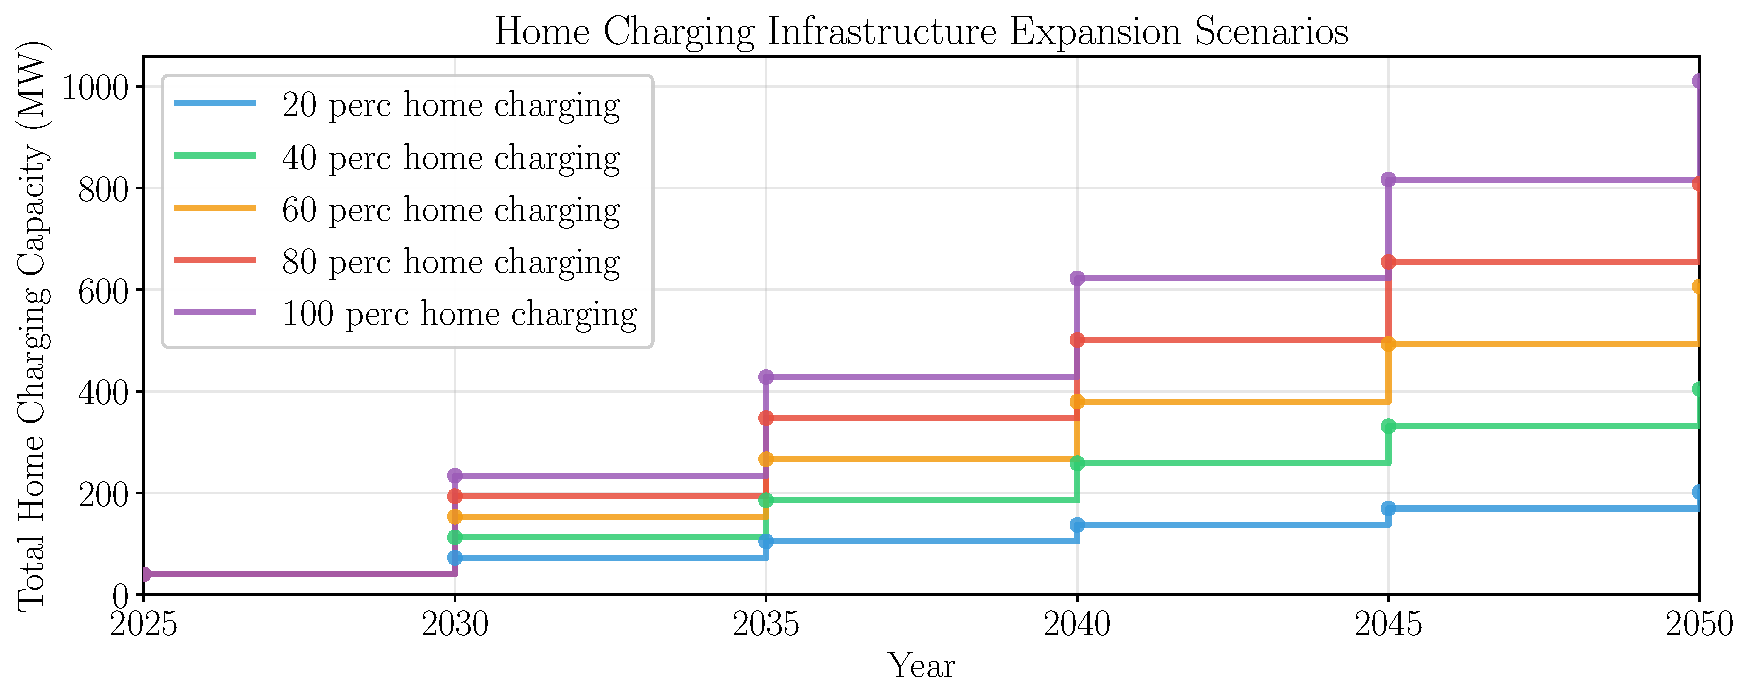
\includegraphics[width=0.9\textwidth]{graphics/home_charging_expansion_scenarios.pdf} 
        \captionsetup{labelfont={color=authorblue}, textfont={color=authorblue}}

    \caption{Scenarios for expansion of home charging (exogenous).} \label{fig: home_charging_exp_scenarios}
\end{figure} 

Figure \ref{fig: SA_comp_cons} displays the impact of increased home charging capacities on the utilization of public charging infrastructure. The increased amount of home charger capacity shifts the charging utilization increasingly to home charging. With this, public charging plays a decreasing role in demand coverage. However, there is no clear patterns visible in the reduction of fast charger utilization. Figure \ref{fig: SA_comp_final} shows capacity installations by charger type for two different years: 2035 and 2045. The increasing home charging capacity is clearly visible. Further, we see that in the case of no fast charger utilization (scenarios \textit{20 perc home charging} and \textit{80 perc home charging}), the public charger capacities are expanded increasingly. 

The unclear trend in fast charging utilization likely reflects near-indifference in the objective function between solutions with and without fast charging.

\textbf{Across all home charging scenarios, the relative differences in adoption timing between income classes persist, confirming that this core finding is robust to home charging assumptions.}

\begin{figure}[H]
    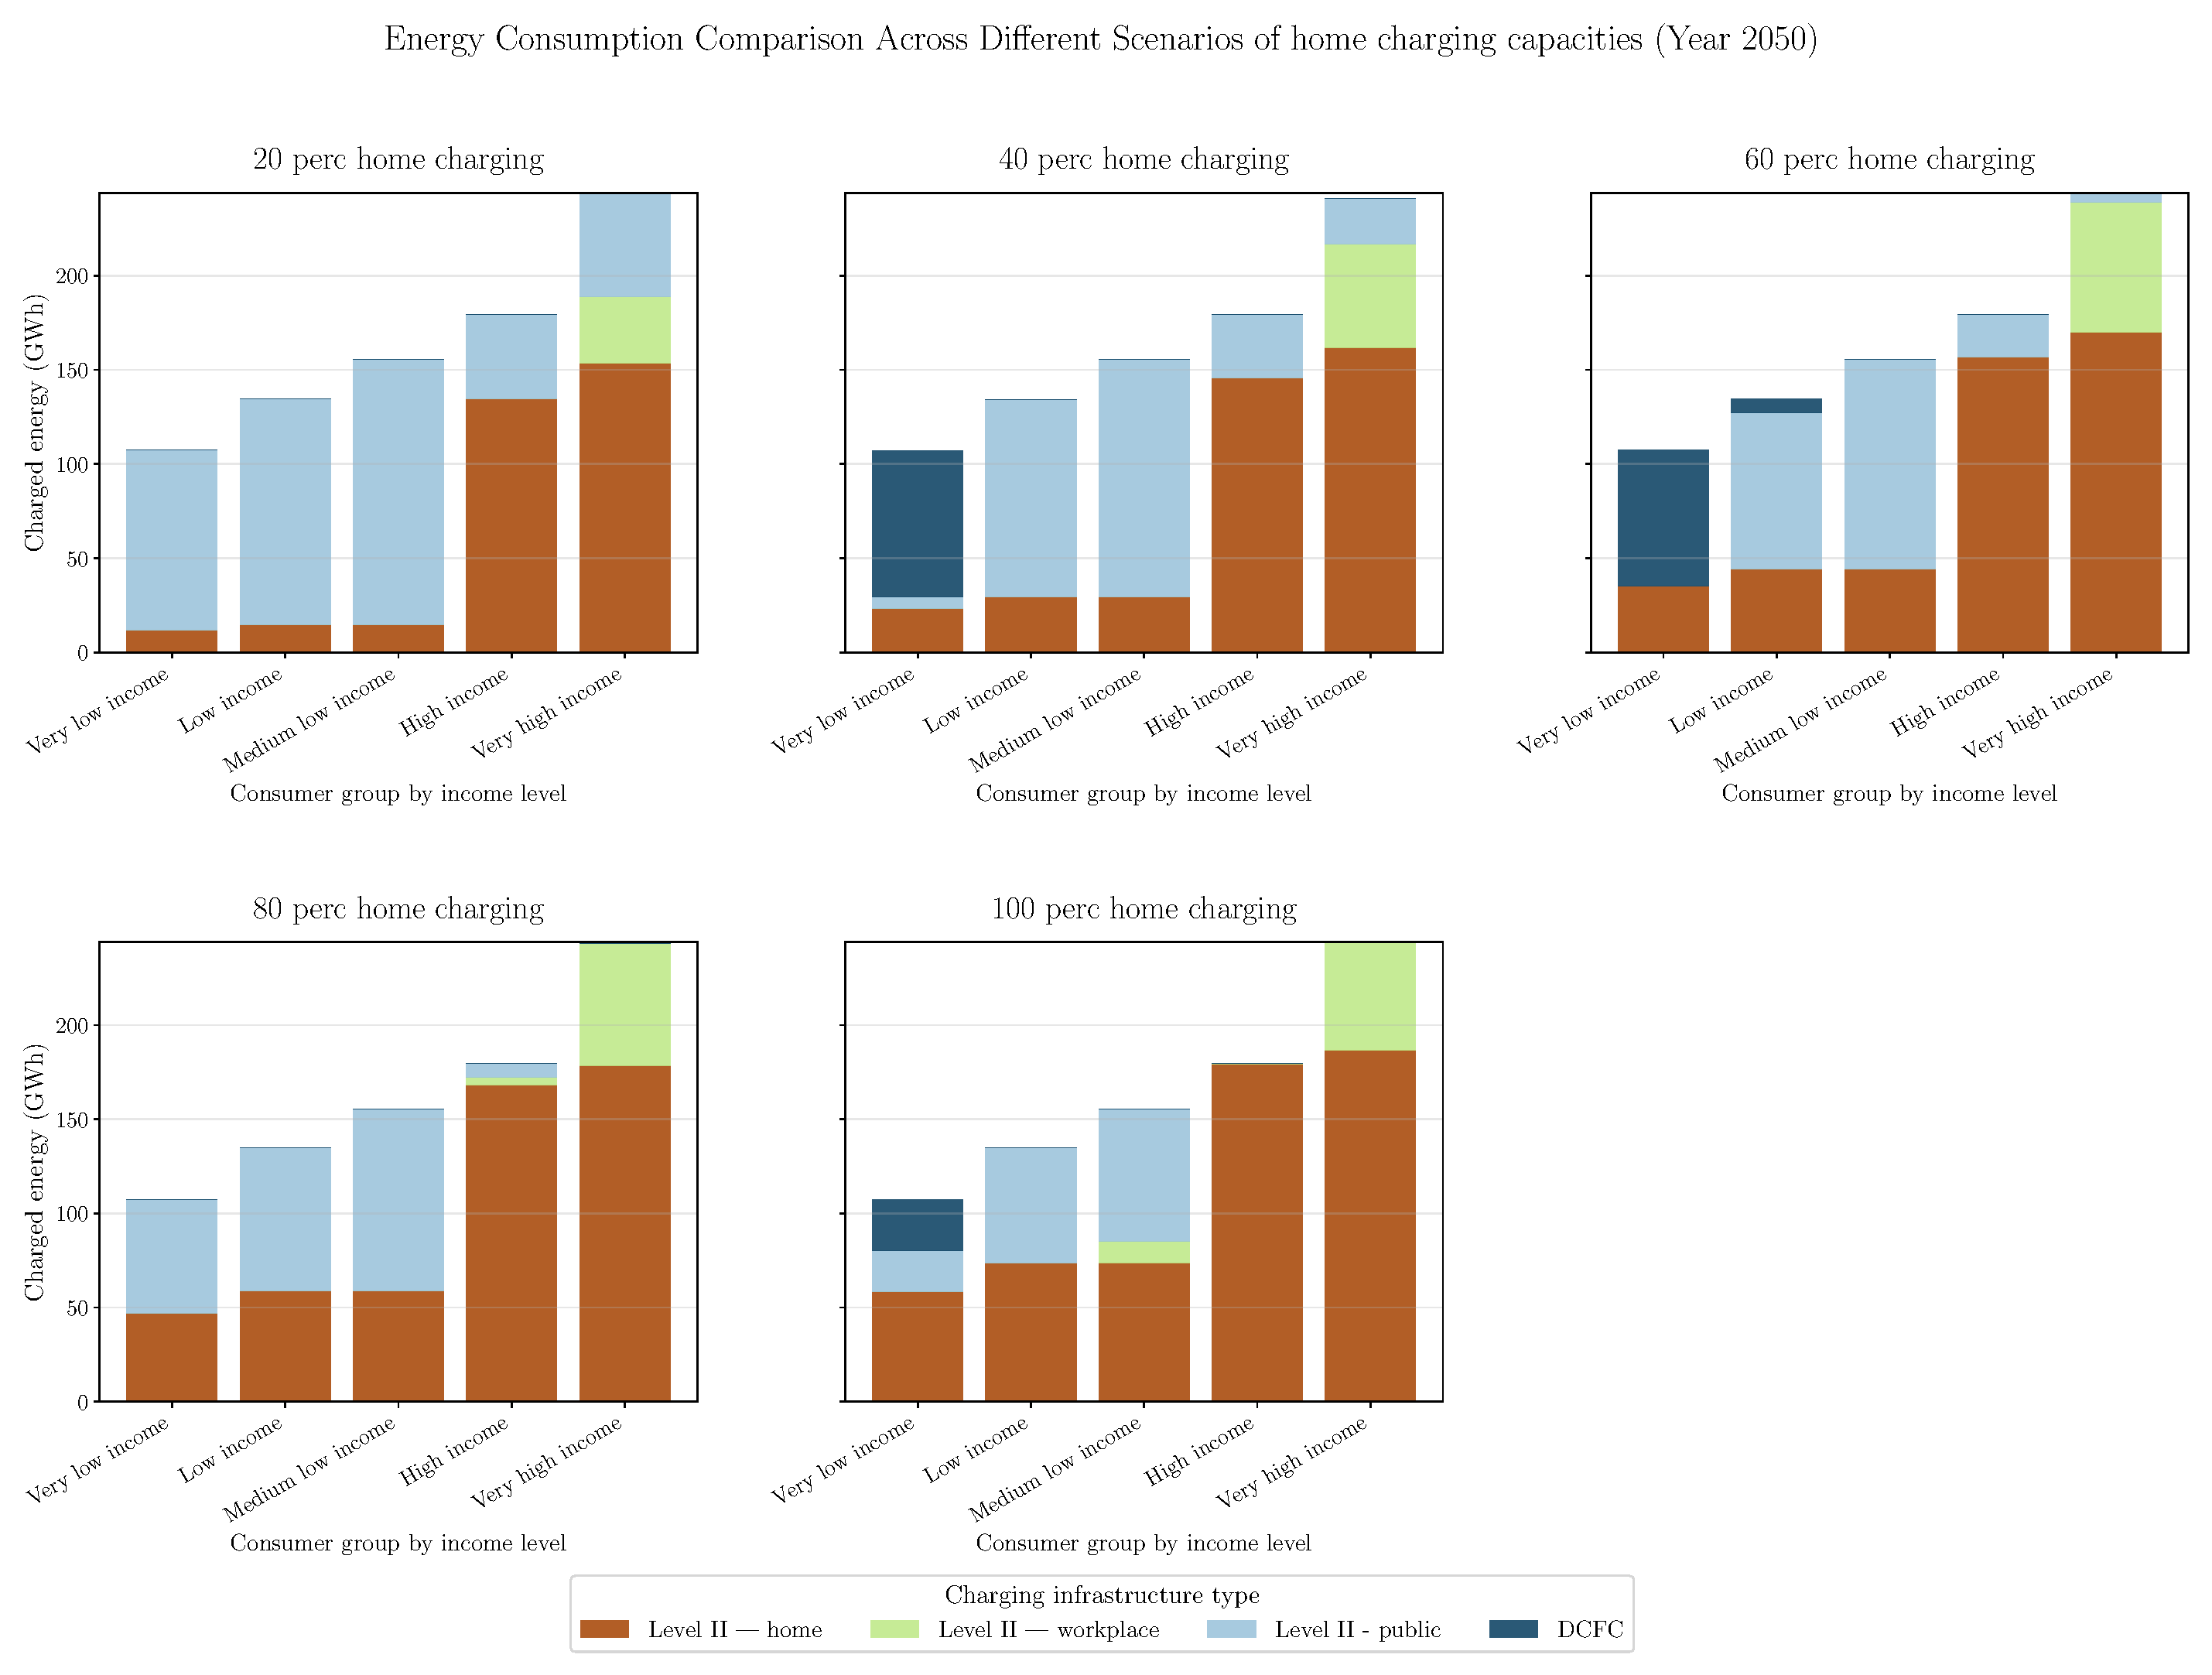
\includegraphics[width=0.9\textwidth]{graphics/SA_comparison_energy_consumption.pdf} 
            \captionsetup{labelfont={color=authorblue}, textfont={color=authorblue}}
    \caption{Comparison of energy consumption patterns across income classes for different cases of exogenously defined home charging capacities.} \label{fig: SA_comp_cons}
\end{figure} 

\begin{figure}[H]
    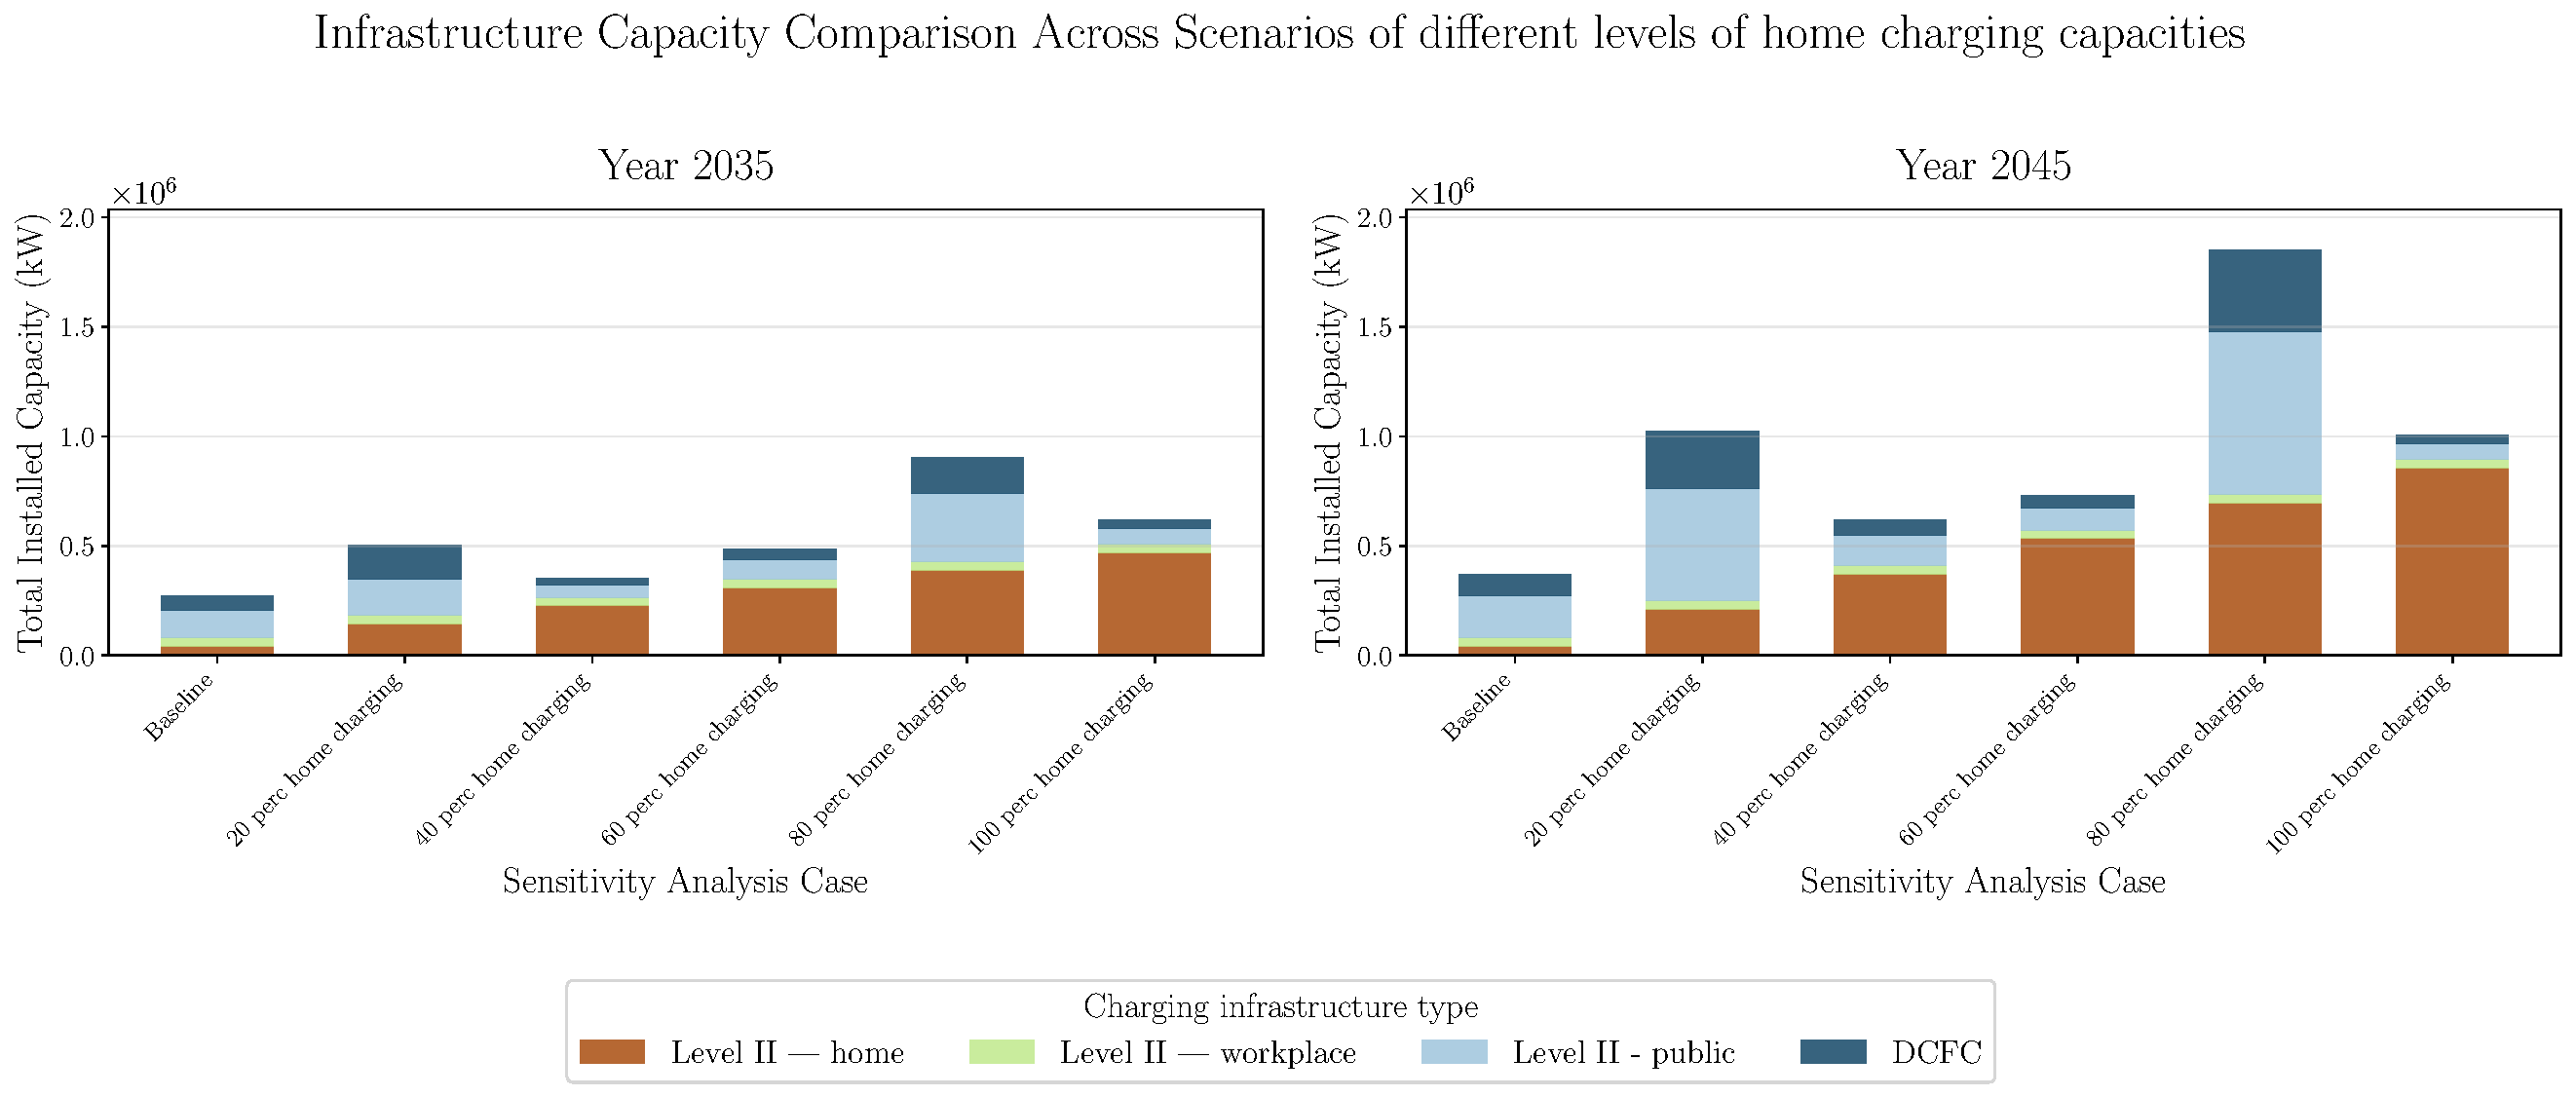
\includegraphics[width=0.9\textwidth]{graphics/SA_comparison_infrastructure_specific_years.pdf} 
            \captionsetup{labelfont={color=authorblue}, textfont={color=authorblue}}

    \caption{Charging infrastructure capacities by charger type installed by years 2035 and 2045 for different scenarios of home charging.} \label{fig: SA_comp_final}
\end{figure} 

\textbf{We have included this sensitivity analysis in the appendix of the manuscript, in Section B.3.}

\color{reviewergrey}
\subsubsection*{4. Fast charging pricing, utilization and economic plausibility \\
\textbf{Issue:} Model results that fast charging has low utilization and that very low income uses fast charging predominantly (because of low VoT) conflict with empirical evidence where fast charging is expensive and tends to be used by specific user profiles. The model currently does not include price heterogeneity or station pricing/markup which will change utilization and adoption incentives. \\ \\
\textbf{Required:}
\begin{itemize}
    \item Discuss and, if possible, include a sensitivity scenario that increases marginal cost/pricing of DCFC (or adds a usage fee) to reflect real world pricing, and show how utilization and equity outcomes change.
    \item At minimum, add a subsubsection investigating how price/markup would change the conclusions.
\end{itemize}
}
\color{authorblue}
\noindent \textcolor{authorblue}{\textbf{Author's response:}}  Thank you for this insightful comment. We agree with the missing representation of pricing structures. This stems from the total-system-cost-minimization approach, which includes monetary budgets for vehicle purchases but not for fueling or charging costs. Within the state of the art that we build on, the necessity of this modeling feature in the context of total-system-cost-optimization approaches has not been addressed yet. This is a significant research gap to be addressed in future work --- in particular, in method frameworks of this kind. Empirical studies \citep{Lanz2022} have highlighted the pricing differences between different charger types. Under realistic pricing where DCFC carries price premiums, lower-income groups would likely shift toward slower, cheaper charging options—reversing the pattern in our results.\textbf{We acknowledge this limitation throughout the manuscript, emphasizing that it arises from our methodological approach and should be addressed in future work.}

By including constraints on the monetary budget for the fueling/charging costs, the charging patterns by different income-level consumer groups would be, therefore, better represented. While we have already mentioned this limitation in the Discussion section (Section 5.1.2), \textbf{we have now extended our statements in order to address the consideration of the potential markup in the modeling. }

\color{reviewergrey}
\subsubsection*{5. Spillover results: magnitude, robustness, and explanation \\
\textbf{Issue:} The spillover to neighbors is reported as modest with a maximum +1.3 percentage-point electrification (by 2040) but the paper stops short of showing robustness, statistical significance, or the mechanism beyond a short explanation about commuter destination charging freeing origin capacity. \\
\textbf{Required:}
\begin{itemize}
    \item Provide more detailed numbers (e.g., absolute BEV counts, percent relative change) and time series plots showing when and how the spillover happens.
    \item Run a robustness check: vary the +30\% accelerated capacity assumption (e.g., +10\%, +50\%) and show how spillover magnitude scales.
    \item Discuss generalizability: with only three NUTS-3 nodes, results may be specific to Basque commuting patterns — authors should explicitly state this and preferably test over a larger set of regions or show why Basque is representative.
\end{itemize}}

\color{authorblue}
\noindent \textcolor{authorblue}{\textbf{Author's response:}}  We fully agree that the spill-over is modest and that the presented results in the original version of the manuscript lack showing the temporal development of this spillover. \\\\
\textbf{Providing detailed numbers:} To provide better insights into the dynamics of the spillover, we have added a Figure (Figure 12) in the Results section (Section 4.2). Following the reviewer's request for more detailed temporal analysis of spillover dynamics, we recalculated the effects with finer resolution and found the maximum spillover impact to be 2.1 percentage points, occurring in 2044. This refined estimate has been updated throughout the manuscript.\\\\
\textbf{Sensitivity analysis:} We address the requested robustness check, by modeling two additional expansion scenarios: One with +15\% of centrally accelerated capacity expansion and one with +45\% expansion to observe how the spillover magnitude scales. Figure \ref{fig: comp_maximum_diff} displays the results indicating the peak of absolute maximum differences between the scenarios \textit{Baseline Roll-out} and \textit{Central Acc. Roll-out}. The impact of increased charging capacity in Bizkaia has an increasingly higher impact on the BEV adoption in Gipuzkoa than Araba. Overall, there is an increasing spillover effect with larger charging capacities in Bizkaia to a similarly modest extend as the main results demonstrate.

\begin{figure}[H]
    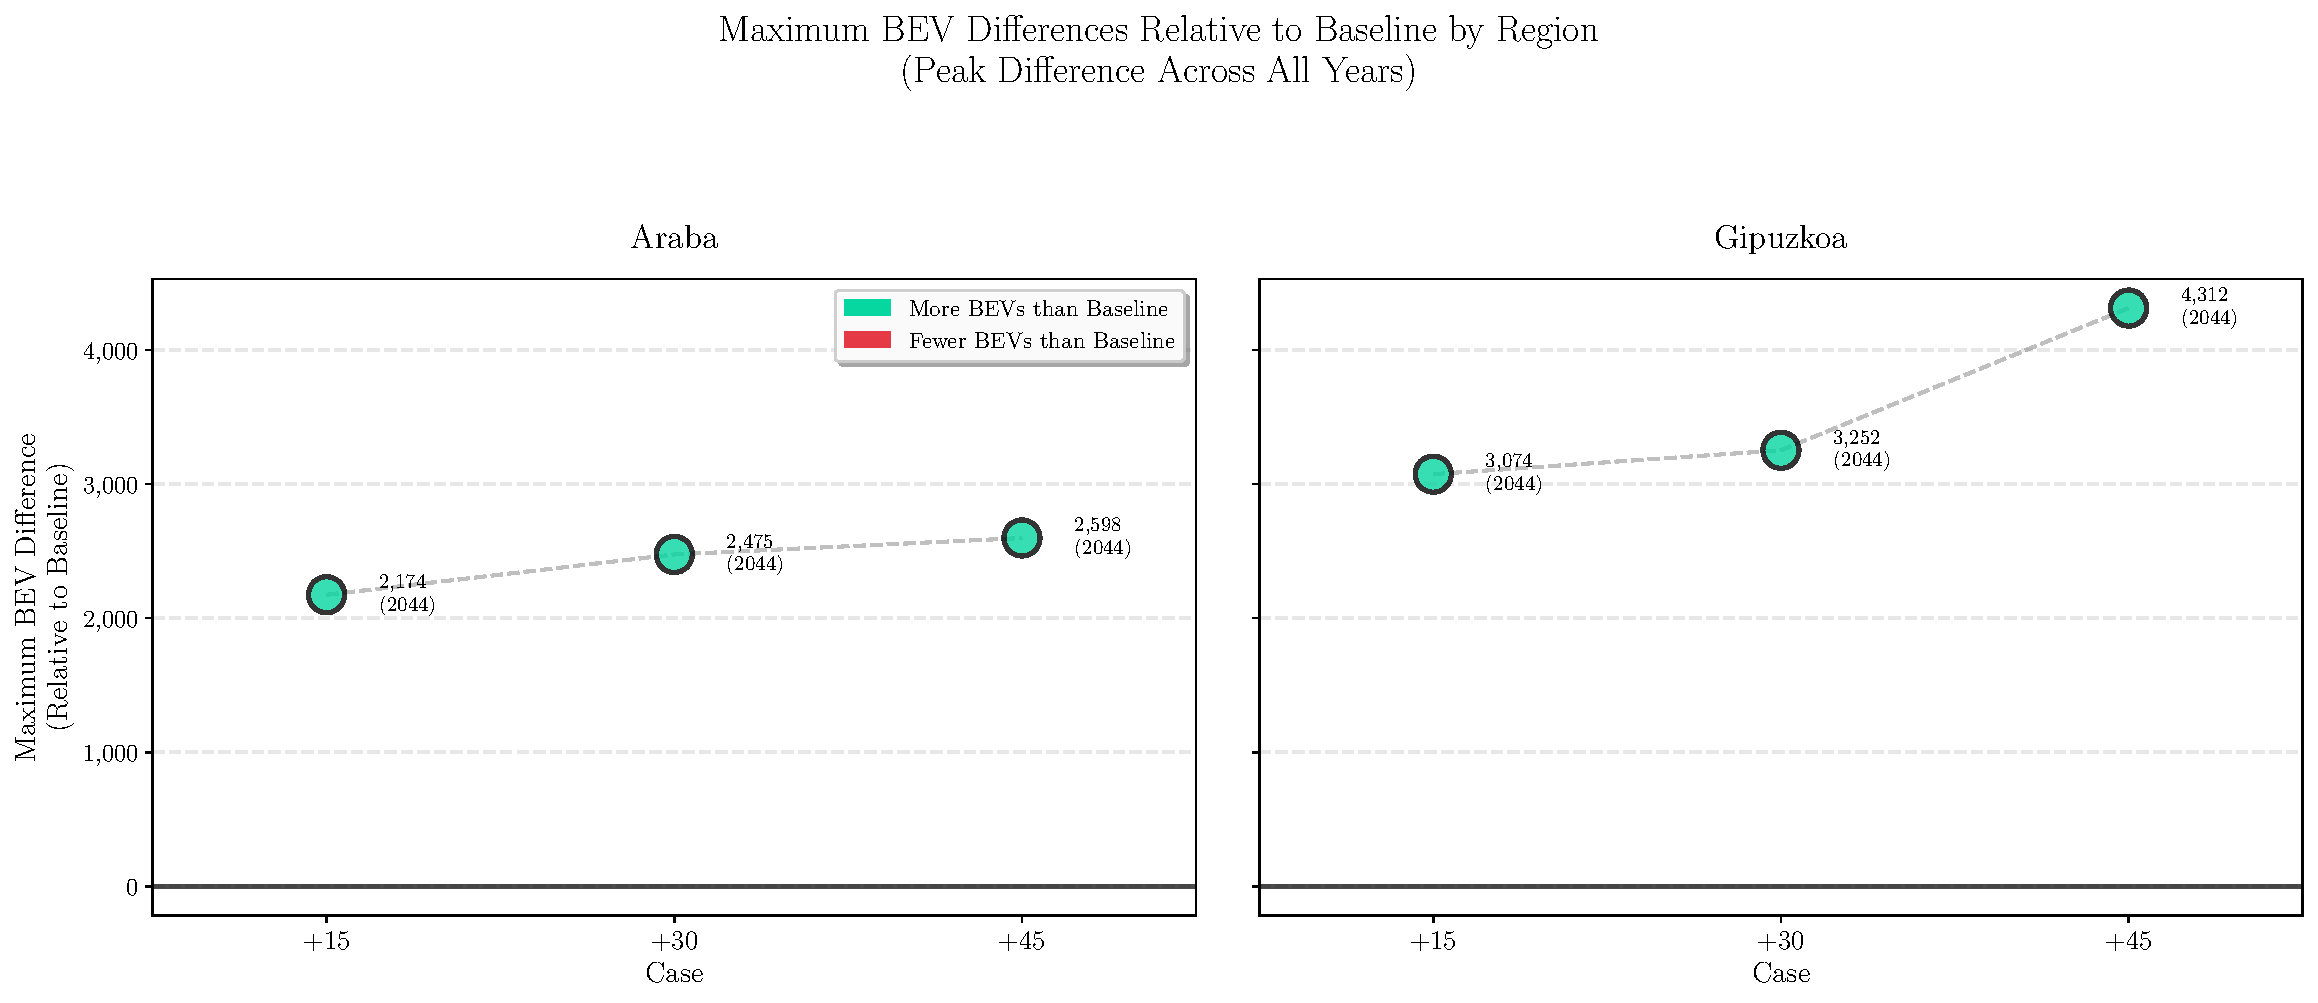
\includegraphics[width=\textwidth]{graphics/h_comparison_maximum_bev_differences_by_region.pdf} 
                \captionsetup{labelfont={color=authorblue}, textfont={color=authorblue}}

    \caption{Peak absolute differences in BEV adoption between Baseline Roll-out and Central Accelerated Roll-out scenarios across capacity expansion levels (+15\%, +30\%, +45\%).} \label{fig: comp_maximum_diff}
\end{figure} 
\textbf{This sensitivity analysis is also included in the appendix of the manuscript.} \\ \\
\textbf{Discussion on generalizability:} We acknowledge that with only three NUTS-3 regions, the spillover results may be specific to Basque commuting patterns. We have added explicit discussion of this limitation in Section 5.2.1 and identify multi-region validation as a priority for future work.

\color{reviewergrey}

\subsubsection*{6. Data vintage and demand growth assumptions \\ 
\textbf{Issue:} Origin-destination trips come from ETISplus (calibrated to 2010) and are scaled using fleet growth and GDP extrapolations. This raises questions about whether mobility patterns (trip lengths, commuting shares) reflect post-2010 realities (telework, modal shifts). \\
\textbf{Required:} Discuss limitations of ETISplus for present/future O-D; where possible validate with more recent sources (national/regional travel surveys or mobile-phone derived OD if available) or at least run sensitivity on total trip growth and commuting share assumptions.
}
\color{authorblue}
\noindent \textcolor{authorblue}{\textbf{Author's response:}} Thank you for raising this important point. There is a lack of availability of open-source data on origin-destination data at this geographic resolution. We use the GDP growth as an indicator for the growth of transport volumes. The GDP growth is a recognized indicator for the growth of transport, and in particular, the private passenger transport \citep{EDELENBOSCH2017281, thomsen2024projecting}. We are convinced that there is a limited value of adding a sensitivity analysis on the absolute numbers of the person-trips and decided to focus in the conduction of sensitivity analyses to likely more impactful model parameters during this revision round. 
As the review comment suggested, \textbf{we have now added have included a short discussion on this limitations in the \textit{Discussion} section (Section 5.2).}
\color{reviewergrey}
\subsubsection*{7. Model transparency, reproducibility, and code/data release \\
\textbf{Issue:} Authors state scripts will be available on request. For a complicated MILP/techno-economic model, full reproducibility is important.
\textbf{Required:} Deposit (or prepare to deposit) the code, preprocessed input datasets (or synthetic equivalents), and solver settings in a public repository (e.g., zenodo/GitHub) or provide detailed appendix pseudocode and data dictionaries. If licensing or privacy prevents raw O-D release, publish sanitized examples and the exact JuMP model files.}
\color{authorblue}
 \noindent \textcolor{authorblue}{\textbf{Author's response:}}  Thank you for this constructive suggestion. We have published the input data files and the source code for the modeling framework \url{https://github.com/antoniamgolab/iDesignRES_transcompmodel}. \textbf{This is now also referenced to in the manuscript.}
\color{reviewergrey}
\subsubsection*{8. Modeling the discrete "lumpiness" and choice of binary variables \\
\textbf{Issue:} The discrete capacity lumps and binary choice of reduction index (w variables) is a modeling choice that must be justified for computational tractability and realism. How sensitive are results to the chosen capi values and number of discrete levels? \\
\textbf{Required:} Provide a short experiment varying the granularity of capi (finer/coarser lumps) and report solution times + changes in key outputs. This helps readers assess whether results are modeling artifacts.
}
\color{authorblue}
\noindent \textcolor{authorblue}{\textbf{Author's response:}}  We sincerely thank your for this observation and fully agree that the discretization of the detour fueling plays an important role in impacting the results. 

The step curve has been derived from the detour fueling time in a way that the number of discrete options would still allow for a solution of the MILP in reasonable time while avoiding a loss in information. We have included a clear description explaining the procedure on the discretization in the Appendix section (Section A.3).

Following your recommendation on a short experiment on the granularity of the discretization, we have tested two sets of detour time reduction curves. These are derived from the detour time function describing the densification of ten points per site (scenario $n^{\mathrm{points~per~site}} = 10$). We have created one coarser and one finer version for both, fast charging and slow charging capacity expansion. Figure \ref{fig: detour_time} displays the curves. The \textit{Baseline} graph indicates the used discretization. 

\begin{figure}[H]
    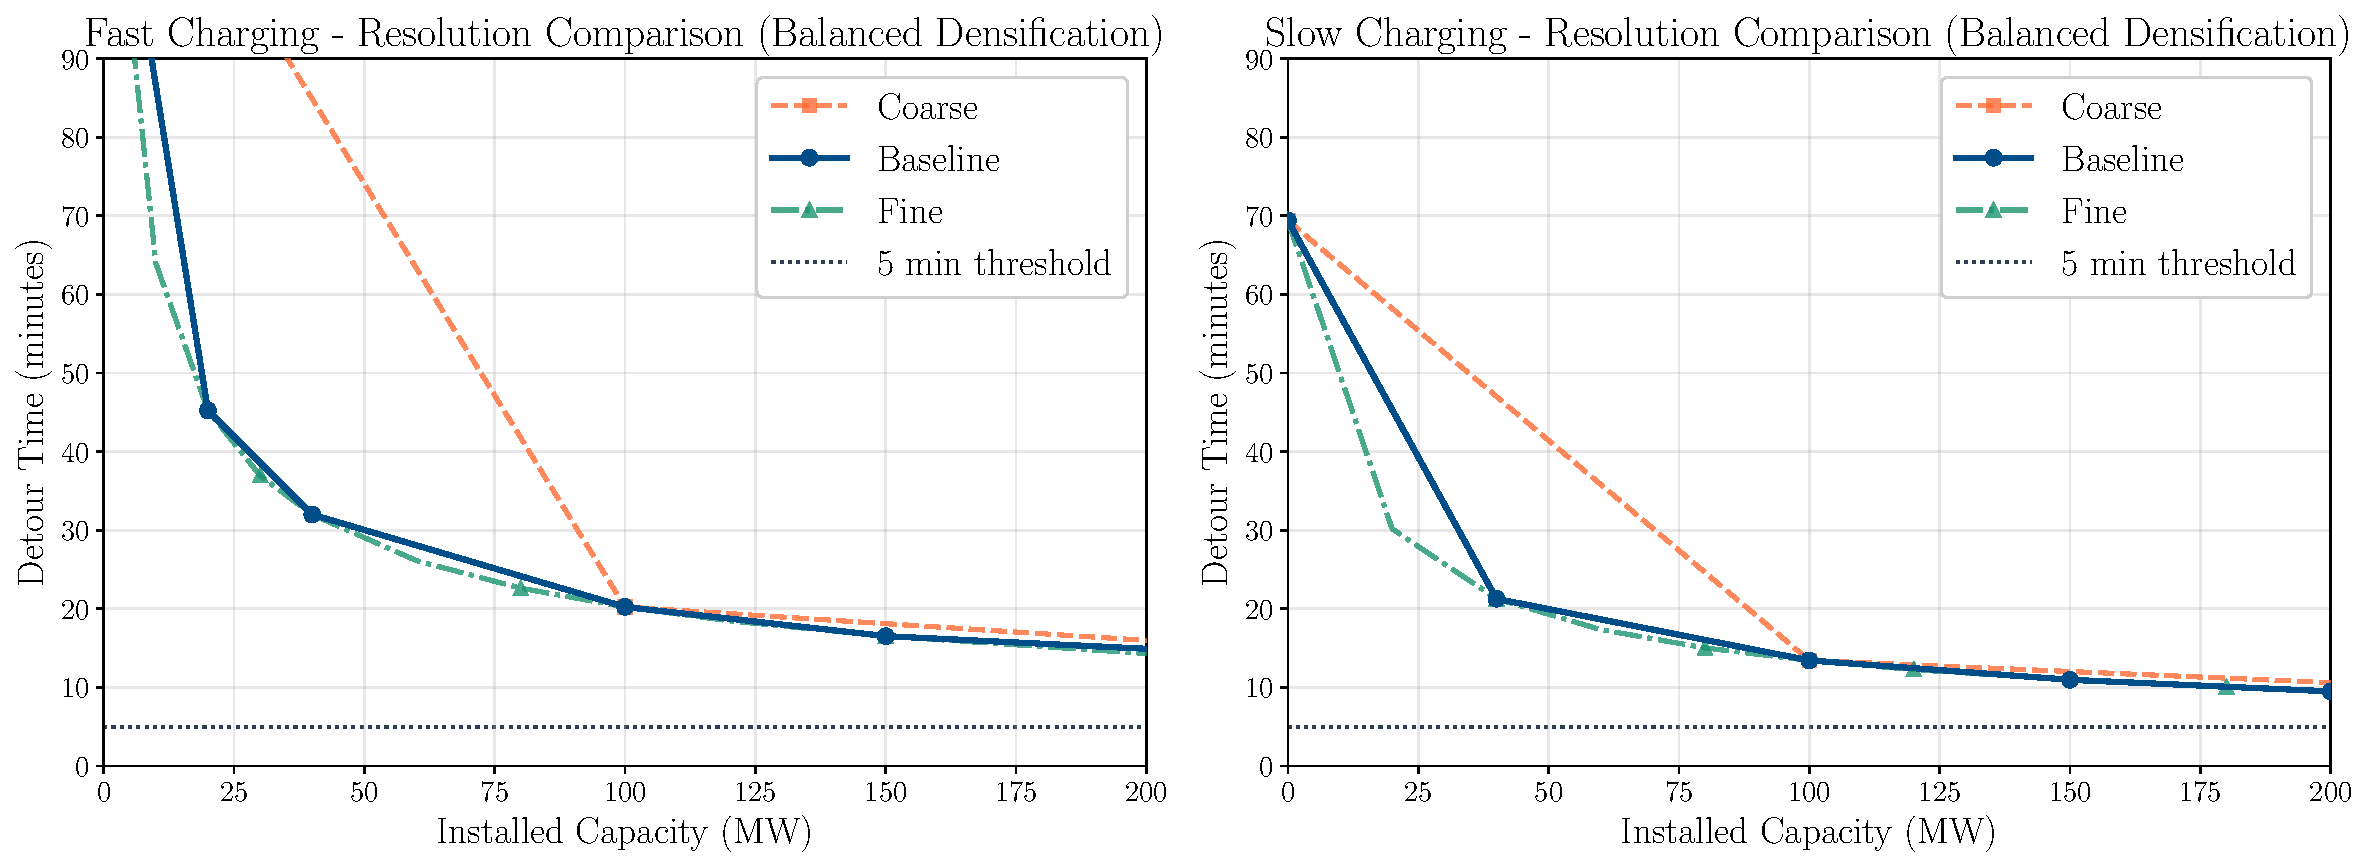
\includegraphics[width=0.9\textwidth]{graphics/detour_time_curves_resolution_comparison_balanced.pdf} 
                    \captionsetup{labelfont={color=authorblue}, textfont={color=authorblue}}

    \caption{Alternative discretization pathways (\textit{Fine} and \textit{Coarse}) for the detour fueling time function compared to the used step size indicated by \textit{Baseline}. } \label{fig: detour_time}
\end{figure} 


\begin{table}[h]
\centering
\caption{Variation of granularity of detour fueling time function discretization: Computation times for initialization, constraint formulation, objective formulation, and MILP solving.}
\label{tab:computation_times}
\begin{tabularx}{\textwidth}{l *{5}{>{\centering\arraybackslash}X}}
\hline
\textbf{Sampling} & \textbf{Initialization (s)} & \textbf{Constraint Formulation (s)} & \textbf{Objective function formulation (s)} & \textbf{MILP Solving (s)} & \textbf{Total (s)} \\
\hline
Coarse & 86.91 & 346.65 & 128.39 & 1008.82 & 1656.50 \\
Baseline & 83.83 & 354.96  & 222.03 & 5739.13 & 6399.95 \\
Fine & 76.59 & 363.13 & 146.39 & 7833.64 & 7690.62 \\\hline
                          
\end{tabularx}
\end{table}

Table \ref{tab:computation_times}, Figures \ref{fig: byincomecons} and \ref{fig:charged_energy} show the results of the experiment. Table \ref{tab:computation_times} summarizes the times of different modeling steps, indicating the increased solution times when the granularity of the discretization is increased. 

Figure \ref{fig: byincomecons} shows little impact on the BEV adoption rates by income classes. Figure \ref{fig:charged_energy} displays the differences in charger utilization by income class in 2050. A significant difference is visible regarding the fast charger utilization which increases in the case of \textit{Finer} resolution of the detouring time function.


\begin{figure}[H]
    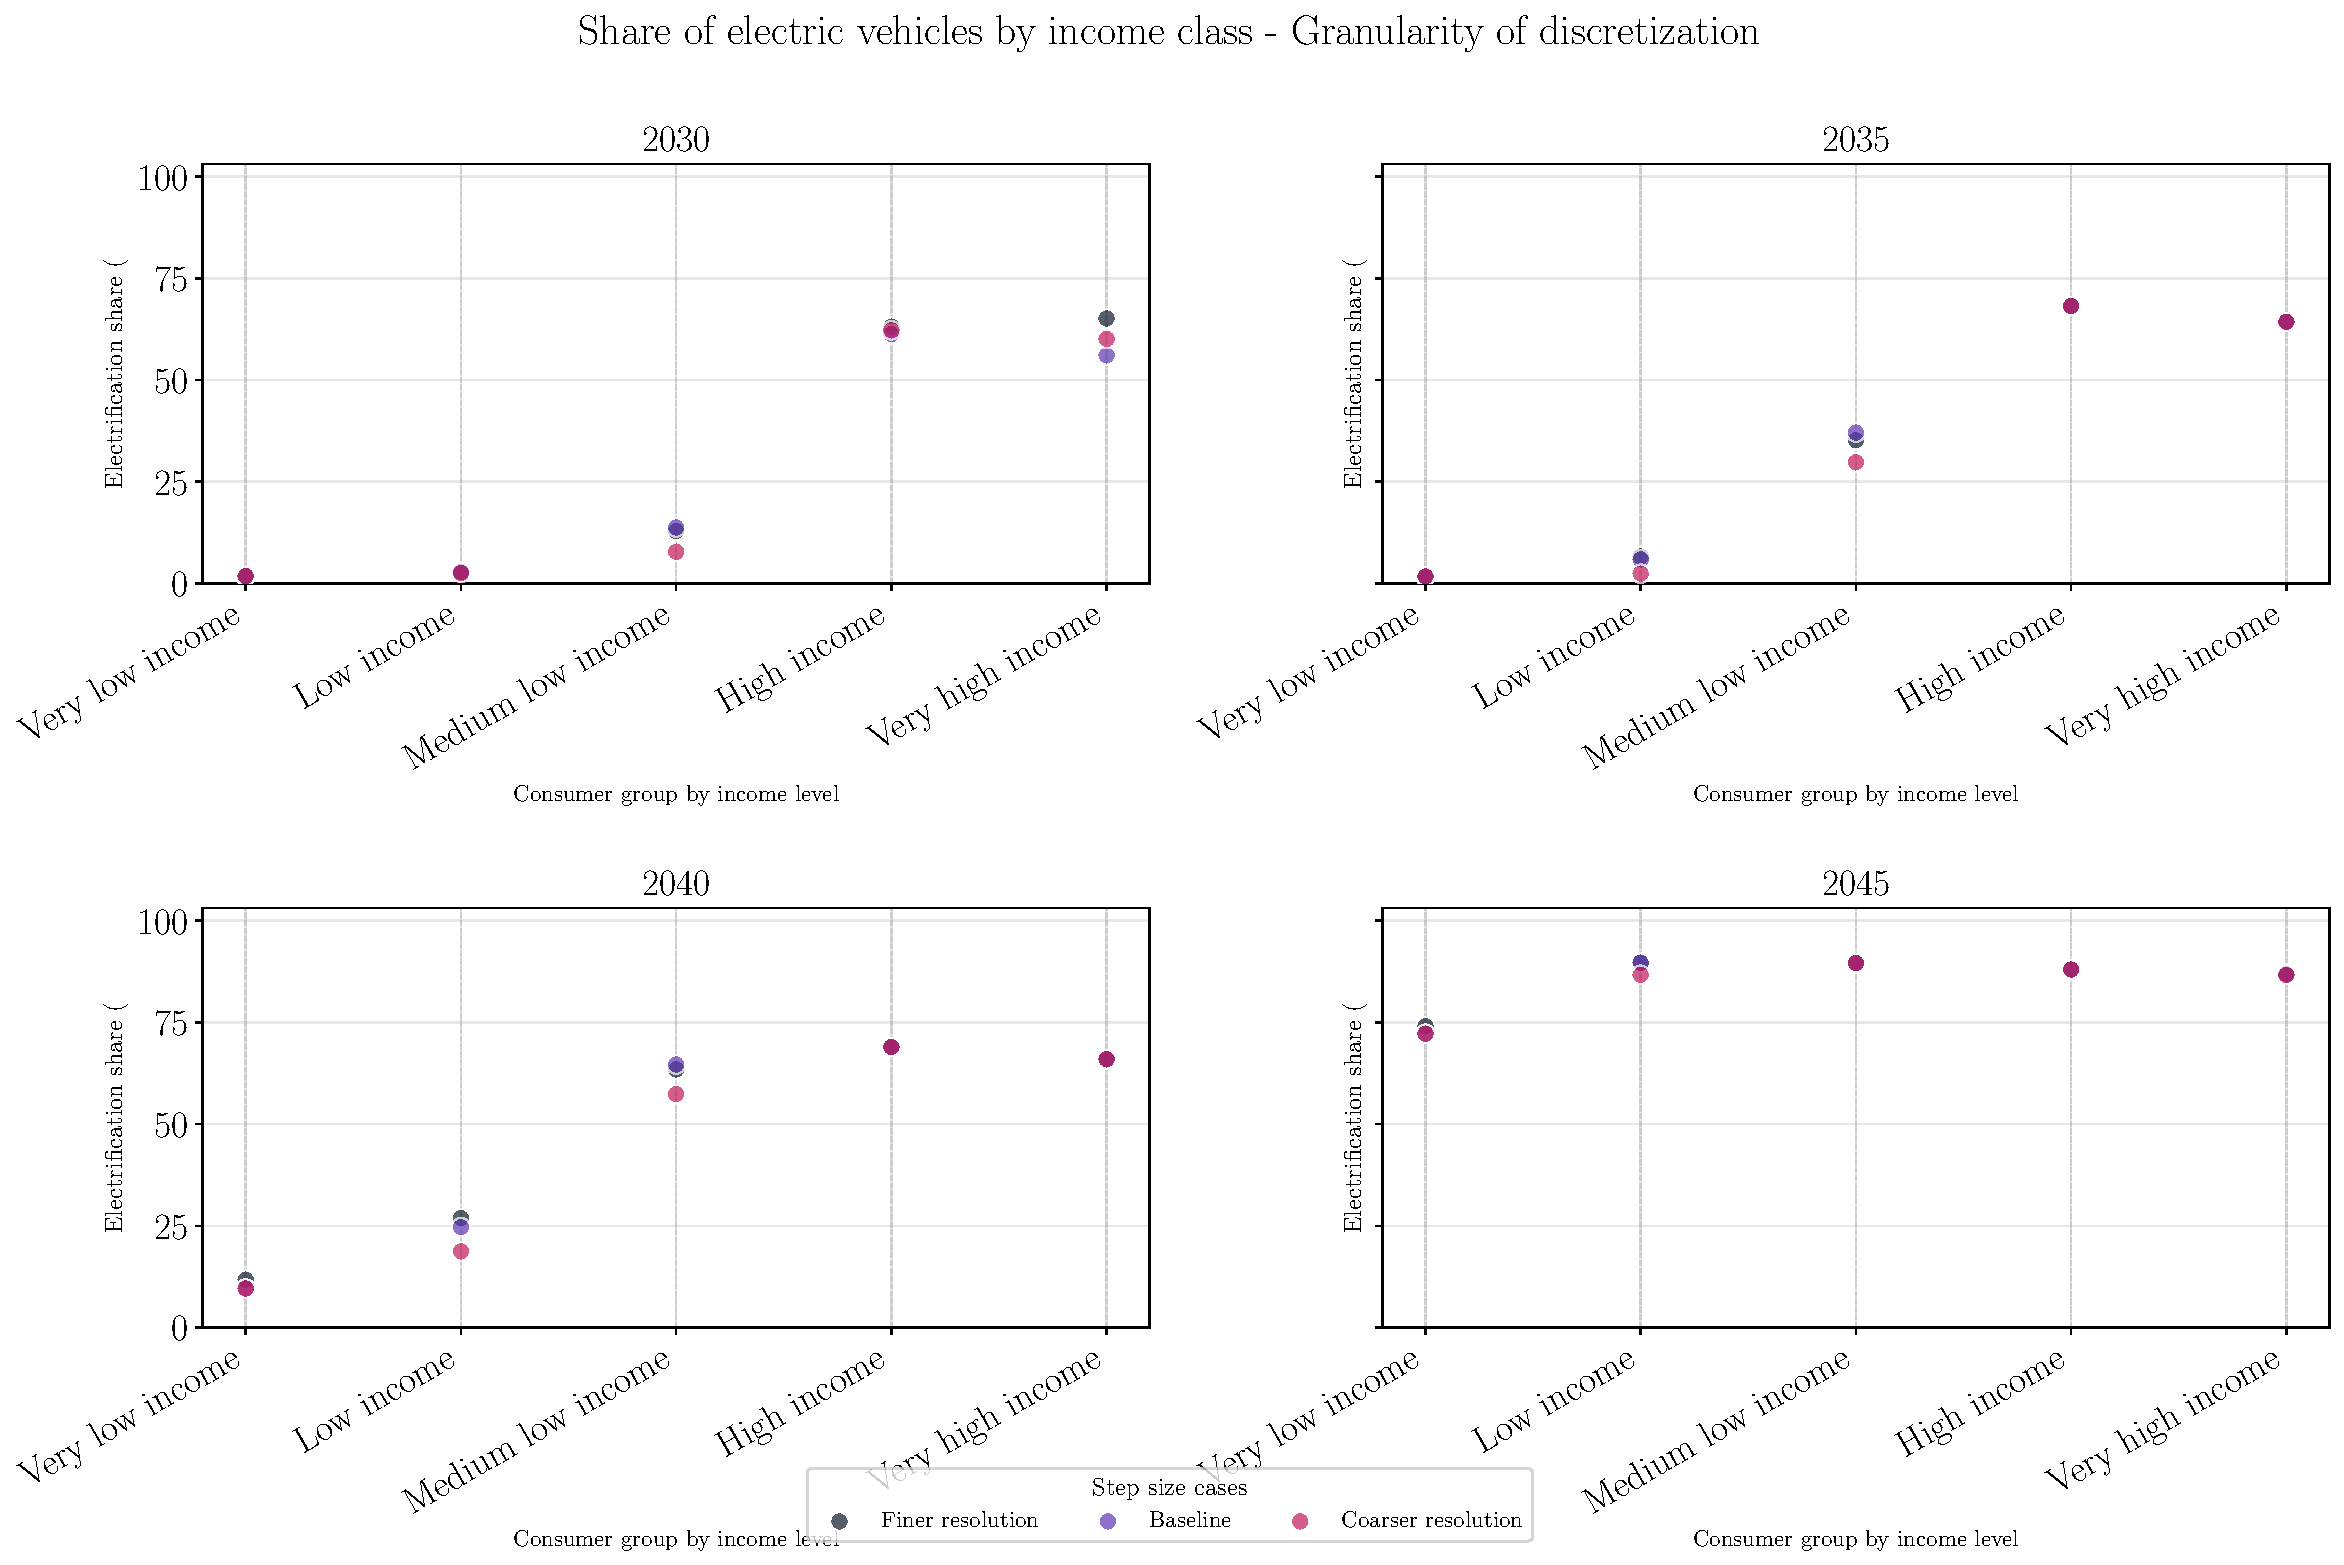
\includegraphics[width=\textwidth]{graphics/SA_alpha_share_electric_vehicles_by_income.pdf} 
                        \captionsetup{labelfont={color=authorblue}, textfont={color=authorblue}}

    \caption{BEV adoption rates by income class under alternative discretization granularities.} \label{fig: byincomecons}
\end{figure} 

\begin{figure}[H]
    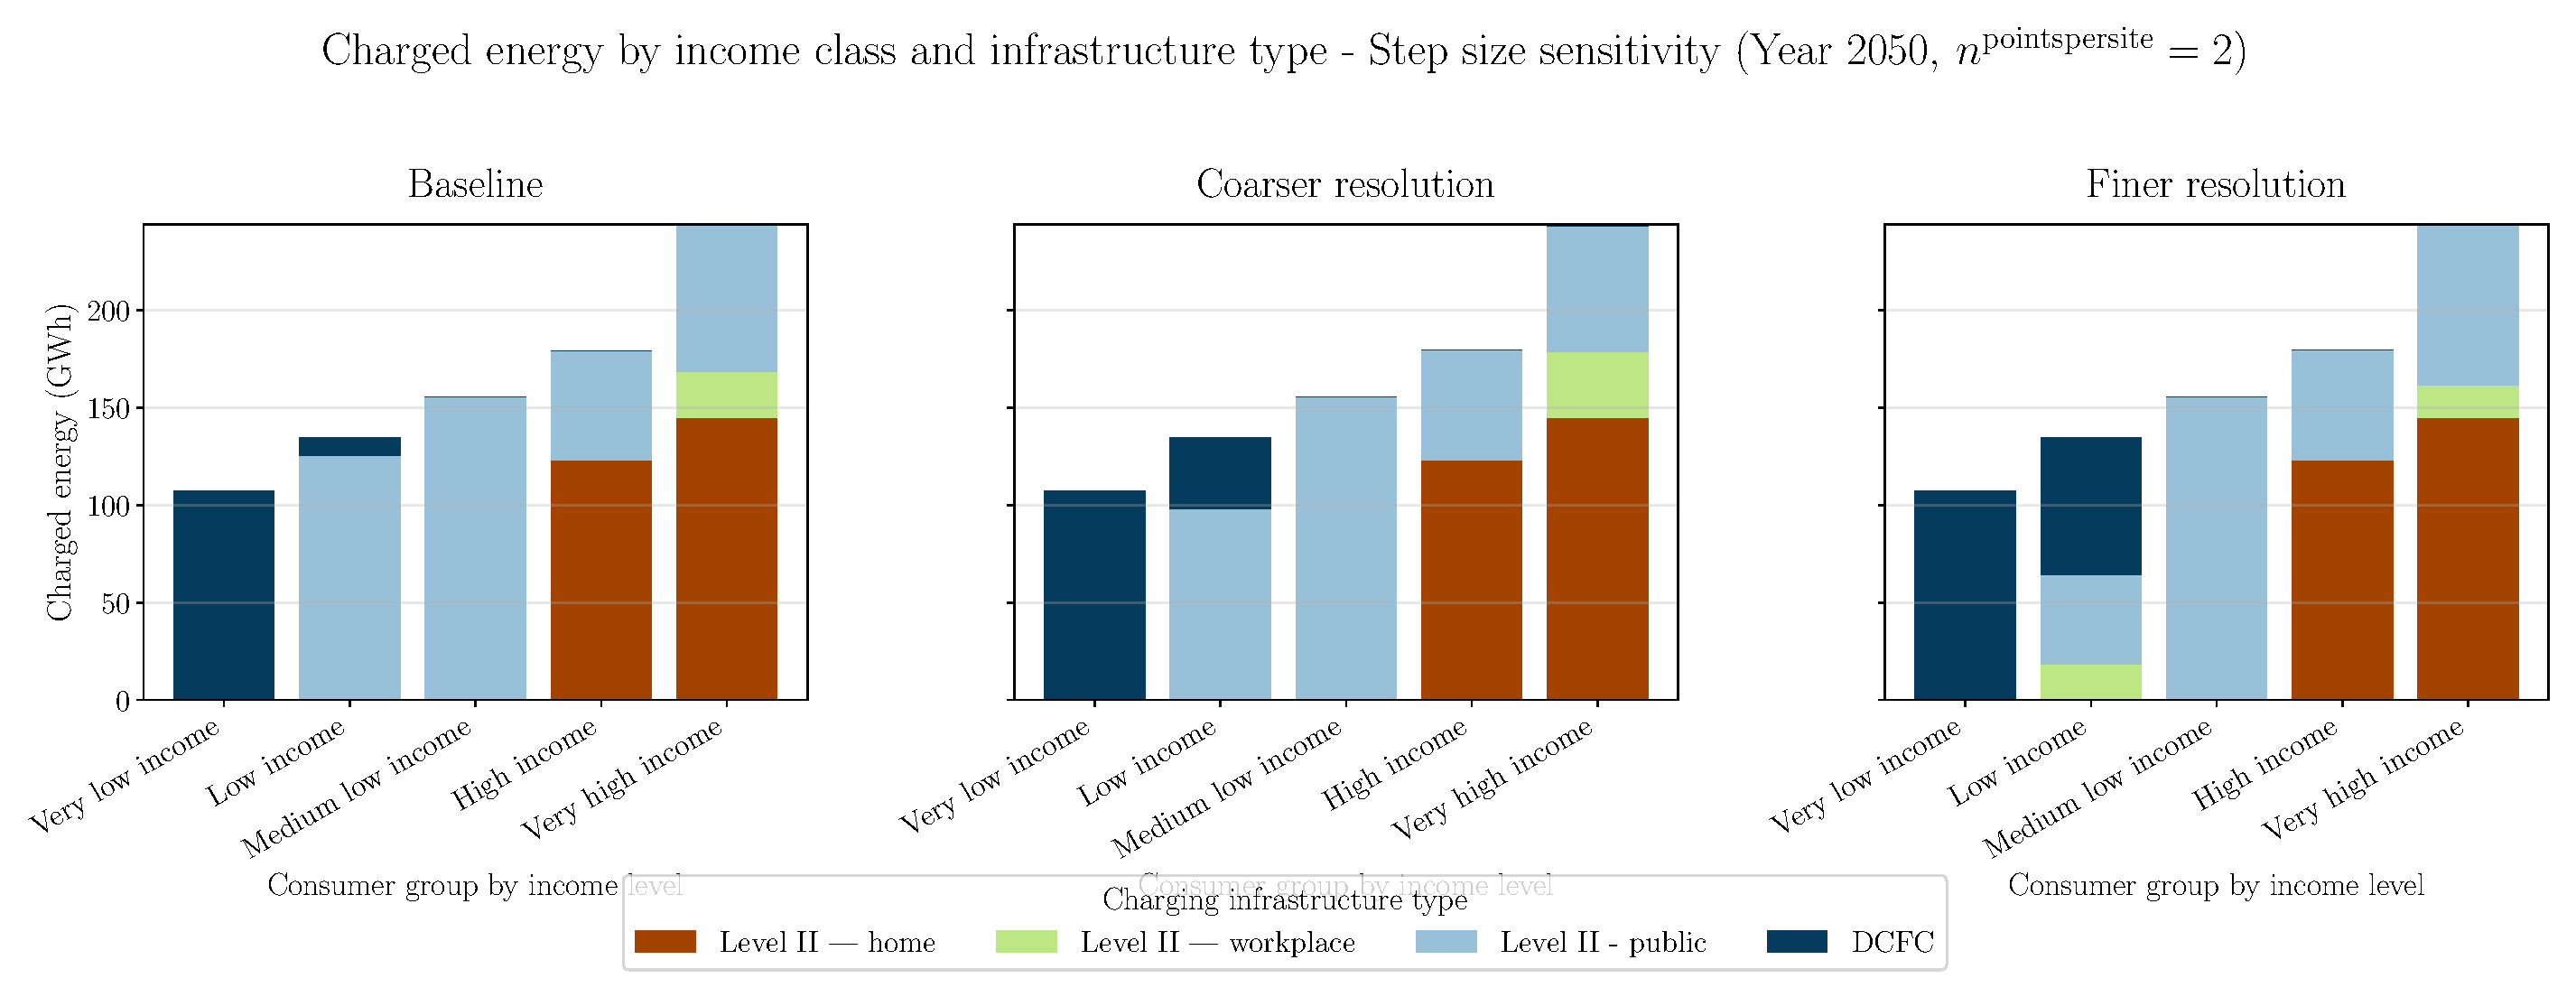
\includegraphics[width=\textwidth]{graphics/SA_alpha_charged_energy_by_income_infrastructure_stepsize.pdf} 
                        \captionsetup{labelfont={color=authorblue}, textfont={color=authorblue}}

    \caption{Final charging infrastructure capacities by charger type under alternative discretization pathways (\textit{Fine} and \textit{Coarse}).} \label{fig:charged_energy}
\end{figure} 

% \begin{table}[h]
% \centering
% \begin{tabular}{lccccc}
% \hline
% \textbf{File} & \textbf{Init (s)} & \textbf{Constr (s)} & \textbf{Obj (s)} & \textbf{Solve (s)} & \textbf{Total (s)} \\
% \hline
% td\_ONENODE\_balanced\_expansion\_alpha\_1\_4\_co... & 86.91 & 346.65 & 128.39 & 1008.82 & 1656.50 \\
% td\_ONENODE\_balanced\_expansion\_alpha\_1\_4\_fi... & 76.59 & 363.13 & 146.39 & 7833.64 & 7690.62 \\
% td\_ONENODE\_concentrated\_expansion\_alpha\_1\_... & 72.98 & 350.92 & 153.39 & 2062.13 & 2724.13 \\
% td\_ONENODE\_concentrated\_expansion\_alpha\_1\_... & 72.95 & 338.77 & 156.58 & 1044.25 & 1683.20 \\
% td\_ONENODE\_concentrated\_expansion\_alpha\_1\_... & 86.86 & 362.65 & 145.14 & 4112.58 & 4794.25 \\
% td\_ONENODE\_distributed\_expansion\_alpha\_1\_4... & 73.94 & 347.80 & 146.63 & 1455.10 & 2111.39 \\
% td\_ONENODE\_distributed\_expansion\_alpha\_1\_4... & 74.11 & 347.07 & 151.89 & 1543.46 & 2203.17 \\
% td\_ONENODE\_distributed\_expansion\_alpha\_1\_4... & 75.09 & 352.81 & 149.36 & 1400.75 & 2067.71 \\
% td\_ONENODE\_distributed\_expansion\_alpha\_1\_4... & 87.24 & 356.31 & 152.14 & 1254.05 & 1936.68 \\
% \hline
% \textbf{TOTAL} & \textbf{706.31} & \textbf{3166.10} & \textbf{1329.90} & \textbf{20914.80} & \textbf{26867.65} \\
% \hline
% \end{tabular}
% \end{table}#
\newpage
\color{reviewergrey}
\textbf{Detailed (line/section) comments and suggestions} \\ \\
\textbf{1. Abstract / Highlights: Good and concise. Consider quantifying the "modest" spillover in the abstract (e.g., "max ~1.3 pp increase in neighboring electrification").}\\ \\
\color{authorblue}
\noindent \textcolor{authorblue}{\textbf{Author's response:}} In accordance with the reviewer's suggestion, we have included the actual number in the Abstract. \\\\
\color{reviewergrey}
\noindent\textbf{2. Section 3.1-3.2 (Model):}
\begin{itemize}
    \item[o] \textbf{Add a short worked example of how the detour variable b is computed for a single representative OD trip to help readers follow the algebra. Cite the constraint equations and show numbers.}
\end{itemize}
\color{authorblue}
\noindent \textcolor{authorblue}{\textbf{Author's response:}} Following your request to increase the reader's understanding of this constraint, we have now included a short numerical example to improve understanding of this constraint.
\color{reviewergrey}
\begin{itemize}
    \item[o]\textbf{ Clarify how occupancy/queueing at chargers is (or is not) modeled. Is there any representation of temporal coincidence (peak hours) beyond $\gamma_l$ peak-factor? If not, discuss implications.}
\end{itemize}
\color{authorblue}
\noindent \textcolor{authorblue}{\textbf{Author's response:}} There is no consideration of queuing and occupancy of the charger beyond the $\gamma_l$ indicator. We clearly mention the annual resolution of the modeling throughout the manuscript. Queuing dynamics are beyond the temporal resolution of our annual model. We note the need for sub-annual modeling as future work in Section 6.\\\\
\color{reviewergrey}
\textbf{3. Section 3.3 (Case study parameterization):}
\begin{itemize}
    \item[o] \textbf{For VoT and budgets, add footnotes showing the specific numeric sources and the scaling method from Denmark→Spain. Also include an uncertainty band.}
\end{itemize}

\color{authorblue}
\textbf{Author's response:}  Thank you for pointing out the missing information on the scaling. We have now included the factor in the Section 3.1.1. An uncertainty band for this VoT values is difficult to define. We address this through the sensitivity analysis presented in the Appendix, Section B.2.
\color{reviewergrey}
\begin{itemize}
    \item[o]\textbf{ Provide more justification for the selection of npoints per site = \{2,10,40\} (why those values? Are they representative?). If possible, compare with observed charging site sizes in Basque/Spain.}
\end{itemize}
\color{authorblue}\textcolor{authorblue}{\textbf{Author's response:}} Thank you for the comment. We have reviewed the scenario description and are convinced that the current description sufficiently describes the decision on the number of points per site chosen.\\\\
\color{reviewergrey}
\textbf{4. Section 3.4 (Scenarios): \\
- For RQ2 scenarios that use $+30\%$ / $-30\%$ capacity changes, add a short sensitivity figure that shows how spillover varies with the percent change (linear or non-linear?). This will help policy readers.} \\\\
\color{authorblue}
\noindent \textcolor{authorblue}{\textbf{Author's response:}} We understand that this comment is building on an earlier comment of the reviewer (Nb. 5 in the previous section of the comments). We have addressed the development by adding a sensitivity analysis with two additional scenarios on additional capacities with \textit{+15\%} and \textit{+45\%} to convey better understanding of potential spillovers.\\\\
\color{reviewergrey}
\textbf{5. Results (Section 4 and 5):} \\
\begin{itemize}
    \item[o]\textbf{ Present absolute as well as relative changes (BEV numbers, share points, and energy demand) so the reader can judge scale (1.3 pp may be small in some contexts and large in others). The paper has some of these but they should be emphasized near the main claims.}
\end{itemize}
\color{authorblue}
\noindent \textcolor{authorblue}{\textbf{Author's response:}} Thank you for this valuable comment. As far as we understand, this comment is also building on comment nb. 5 in the previous section which is concerned with the request for better understandability of the spillover results. Following the previous comment, we have included a figure showing the absolute number of BEVs and the magnitude of spillover effects through 2050 (Figure 12).
\color{reviewergrey}
\begin{itemize}
    \item[o]\textbf{Add a short subsubsection linking utilization rates to economic feasibility (OPEX recovery): e.g., if DCFC utilization maxes at 6-11\%, is that financially realistic for private operators? Discuss policy consequences.}
\end{itemize}
\color{authorblue}
\noindent \textcolor{authorblue}{\textbf{Author's response:}} We appreciate this suggestion. While our system optimization framework does not explicitly model charging prices, we have critically acknowledged empirical pricing differences. Given the manuscript's length, we have limited additional citations but acknowledge this as relevant context.\\\\
\color{reviewergrey}\textbf{6. Limitations (Section 5):}
\begin{itemize}
    \item[o]\textbf{ Authors already discuss multiple limitations; good. But several items flagged there should be shifted to concrete future work experiments (e.g., multi-region analysis, explicit commuter isolation) and placed in a "required sensitivity checks" list rather than only in limitations.}
\end{itemize}
\color{authorblue}
\noindent \textcolor{authorblue}{\textbf{Author's response:}}
We have revised the Discussion (Section 4) and Conclusion (Section 6) to reframe key limitations as concrete directions for future work. Specifically, we now identify multi-region analysis and explicit modeling of commuter flows as priority extensions, rather than listing them solely as limitations. \\\\
\color{reviewergrey}
\textbf{7. Figures and Tables:}
\begin{itemize}
    \item[o] \textbf{Figures that show time series (detour/time, adoption by income) are central — ensure axis labels, units and legends are readable at journal size. For figure 4 and figure 11 the compressed axis labels in the PDF are hard to read; consider splitting panels or enlarging labels.}
\end{itemize}
\color{authorblue}
\noindent \textcolor{authorblue}{\textbf{Author's response:}} We have included one supporting figure displaying the temporal dynamics of BEV adoption (Figure 12) and have increased the font size of text displayed in Figures 13 and 14.\\\\ \color{reviewergrey}
\textbf{8. References / recent work:}
\begin{itemize}
    \item[o]The literature review is thorough. Consider citing a few recent empirical works on charger occupancy and pricing to support discussion of DCFC economics and tariff effects (authors cite Lanz et al.; consider adding regional operator reports where relevant). 
\end{itemize}
 
\color{authorblue}\noindent \textcolor{authorblue}{\textbf{Author's response:}} We appreciate this suggestion. While our system optimization framework does not explicitly model charging prices, we have acknowledged empirical pricing differences by citing \cite{Lanz2022} and added interpretive caution regarding DCFC utilization patterns in Section 5.1.2. Given the manuscript's length, we have opted not to expand the literature review further but recognize this as relevant context for future work. \\\\
\color{reviewergrey}
\textbf{Minor edits}\\
\textbf{* A few typos and formatting glitches occur (e.g., repeated text around first pages); please run an editorial pass. The preprint date appears to be September 28, 2025 — verify dates in references that cite 2025 sources. }\\\\
\color{authorblue}
\noindent \textcolor{authorblue}{\textbf{Author's response:}} Thank you for noticing that there are still typos included. We have carefully checked the text and corrected typos and formatting glitches. \\\\
\color{reviewergrey}\textbf{* In Table 4 (income classes) consider adding a short rationale column explaining how "home ownership" percentages were assigned (currently explained in text, but a one-line justification in the table would help).}\\\\ 
\color{authorblue}\textbf{\noindent \textcolor{authorblue}{\textbf{Author's response:}} We have added a sentence explaining this assumption more clearly. \\\\
\color{reviewergrey}
\textbf{Suggested additional experiments}} \\\\
\noindent \textcolor{authorblue}{\textbf{Author's response:}} Thank you for summarizing the suggestions for additional experiments. We assume that the following comments are shorter descriptions of the comments in the first comment section of the reviewer. Therefore, in the following we just shortly state how the respective comment/suggestion has been implemented.\\\\
\color{reviewergrey}
\textbf{1. g(q) robustness: Replace the current detour function with (a) empirical sampling of charger locations, (b) exponential decay, and (c) more clustered (urban-biased) siting. Report BEV adoption and utilization results.} \\\\
\color{authorblue}
\noindent \textcolor{authorblue}{\textbf{Author's response:}} We have added the testing of alternative $g(q^{fuel\_infr, +})$ functions and observed the output of the BEV adoption and charger utilization among the income classes. \\\\
\color{reviewergrey}
\textbf{2. VoT bounds: Re-run main scenarios with VoT ±30\% per quintile. Report changes in electrification and charger usage.} \\\\
\color{authorblue}
\noindent \textcolor{authorblue}{\textbf{Author's response:}} We have conducted sensitivity analysis using different absolute and relative values of the VoT parameter for one scenario and report on the changes in electrification and usage of charger types across the different income classes.\\\\
\color{reviewergrey}
\textbf{3. Pricing scenario: Add a DCFC tariff scenario (+euro/kWh or euro/min) and show its effect on utilization and equity outcomes.}\\\\
\color{authorblue}
\noindent \textcolor{authorblue}{\textbf{Author's response:}} As our modeling framework does not consider the actual pricing of different fuels but is a total cost minimization, we have not conducted a sensitivity analysis on different tariffs. However, we discuss the limitation of this modeling feature in the Discussion section (Section 5.2.): \say{While public slow charging has a central role in the coverage of the charging demand, public fast charging infrastructure has low utilization rates and is exclusively used by the \textit{Very low income} consumer group. This can be due to two reasons: First, detouring times are systematically higher for public fast charging, and the charging process itself is considered as lost time within the simulation. For the \textit{Very low income} consumer group, the value of time is sufficiently low that time spent on fast charging does not significantly reduce the perceived level of service of BEVs. This holds true for all roll-out scenarios. This is in contradiction with empirical research, which indicates high prices in fast-charging \citep{Lanz2022}. }
Further, in our Conclusion section (Section 6), we clearly state how the future work should be directed towards addressing this limitation: \say{Part of future work must be an improved representation of consumer-group-specific monetary constraints, particularly with regard to operating costs [\dots].} \\\\
\color{reviewergrey}
\textbf{4. Home expansion scenario: Force home charging availability to a higher cap (e.g., 50\% of homeowners) and show outcomes on public charger needs.} \\ \\
\color{authorblue}\noindent \textcolor{authorblue}{\textbf{Author's response:}} We have included sensitivity analysis with five elevated home charging capacities that are exogenously introduced to the modeling. The results on this are also included in the Appendix (Section B.3).\\\\
\color{reviewergrey}
\textbf{5. Multi-region check: If feasible, run a second (smaller) case study for a different NUTS-2 region or synthetic three-region system to test generality of spillover findings.}\\\\
\color{authorblue}
\noindent \textcolor{authorblue}{\textbf{Author's response:}} We believe that the inclusion of this is out of scope of the current work. This is not feasible without major additional computational efforts while the benefit and insights would be marginal to the conclusion. We have included this as a direction for future work. \\\\
\color{reviewergrey}
\textbf{Final assessment / editorial recommendation\\
This manuscript addresses timely and policy-relevant questions with an interesting integrative modeling approach (detour as endogenous, income segmentation, cross-region spillovers). The work is promising and will be of interest to TRD readers, but several substantive methodological and empirical grounding issues must be addressed before publication, in particular (i) calibration and sensitivity of the detour→capacity relationship, (ii) VoT/data calibration and sensitivity, (iii) representation of home charging and DCFC pricing/feasibility, and (iv) clearer and more robust presentation of the spillover magnitudes and mechanisms. After those revisions and additional robustness tests, the paper would likely be publishable.} \\\\
\color{authorblue}
\noindent \textcolor{authorblue}{\textbf{Author's response:}}  Thank you for the extensive review and the clearly formulated suggestions for improving our manuscript. Following your comments, we have now extended the manuscript to accommodate an increased amount of sensitivity analysis to increase the robustness of the modeling insights. Each of the points (i)-(iv) has been addressed through the presentation and discussion of sensitivity results and, we trust that the thorough revisions have resolved the issues raised and that the manuscript is now ready for publication. 
\newpage
\fancyhead[L]{\textit{Response to Reviewer \#2}}
\color{reviewergrey}
\section*{Reviewer \#2}
\textbf{The paper develops a regional co-planning optimization that jointly determines passenger-car technology adoption and charging-infrastructure deployment for Spain's Basque Country, segmenting five income classes by value of time and budgets and linking added public capacity to reduced detour and charging time through a piecewise function. The authors find that denser public networks reduce detours, direct-current fast-charging (DCFC) utilization is low and concentrated among the very-low-income group, and lower-income consumers appear less sensitive to added charging and detour time under the study's value-of-time assumptions. The topic is timely, the co-optimization with income segmentation is useful for planning, and the writing and mathematical exposition are generally clear. I recommend acceptance with minor revisions.} \\\\ 
\color{authorblue}\noindent \textcolor{authorblue}{\textbf{Author's response:}} 
Thank you for your positive assessment and constructive suggestions. We have addressed each comment as detailed below and believe these revisions have further strengthened the manuscript.
\\
\color{reviewergrey}
\subsubsection*{1. The equity takeaway should be framed explicitly as a model-conditional implication of the value-of-time inputs rather than as an empirical behavioral finding. The paper imports income-specific value-of-time parameters from a Danish case study (Tattini et al., 2018), scales them to the Basque Country, and uses those inputs to monetize time; this choice plausibly drives the result that lower-income groups tolerate longer charging and detours. The authors should state this conditionality where results are presented and, if feasible, add a short sensitivity (e.g., $+-$25\% on value-of-time by income or from a second literature source) to show that the results are robust to these uncertain inputs.}
\color{authorblue}
\noindent \textcolor{authorblue}{\textbf{Author's response:}} 
Thank you for pointing out this important framing issue. We have reframed the equity-related findings to emphasize their dependence on VoT assumptions in Section 5.1.1 (Discussion) and Section 6 (Conclusion).

\textbf{VoT assumption:} Due to the lack of region-specific data for the Value of time (VoT) for different consumer groups, we have drawn from data for Denmark based on a published study by \citet{TATTINI2018265}. The reasoning behind the usage of the data by \citet{TATTINI2018265} is twofold: First, the availability of a range of values that specifically describe different levels of income. Second, the study by \citet{TATTINI2018265} applied these values in a methodologically similar manner, which also informs the foundation of our approach. \\ 
Concerning the scaling that is mentioned in this comment, we base the usage of the Purchase Power Parity measure for the conversion of the values between the countries based on the publication by \citet{WARDMAN201693}. The authors explicitly address the main determinants of the VoT by comparing studies from different countries and applying exploratory analysis to identify relevant parameters that lead to the country/study differences. They identify the cost of living, type of trip and mode type to be the most relevant influencing parameters. We are, therefore, confident that our assumed VoT values by income class reflect the VoT values of Spain.

\textbf{Sensitivity analysis:} In accordance with the recommendation, we conducted additional sensitivity analysis to assess the potential impact of the parameterization of the VoT values. In the design of the sensitivity analysis, we tackle two aspects: Different absolute values and relative differences between the income classes. The following two figures display the tested VoT scenarios (Figure \ref{fig: VoT_tesing_2}):

\begin{figure}[H]
    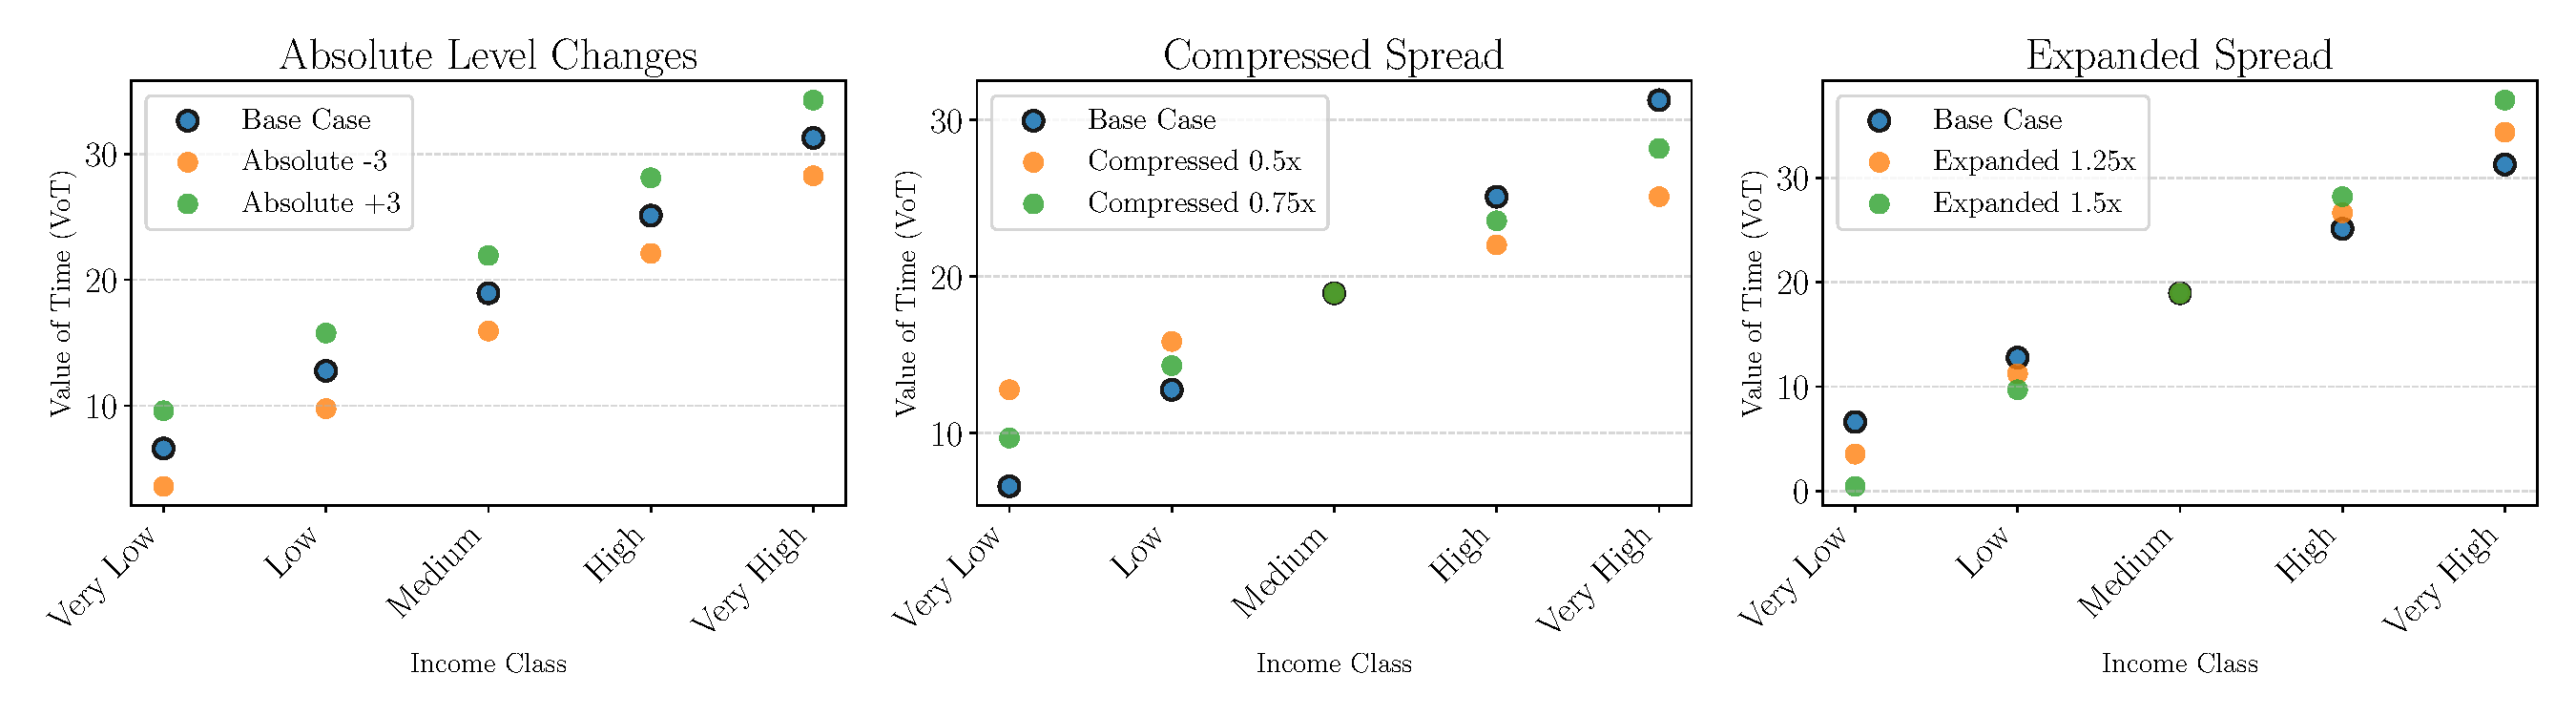
\includegraphics[width=\textwidth]{graphics/sensitivity_analysis_vot.pdf} 
    \captionsetup{labelfont={color=authorblue}, textfont={color=authorblue}}
    \caption{The \textit{Base Case} displays the assumed VoT values for the Basque country. \textit{Left:} VoT values for absolute increase and decrease of the value of time. \textit{Center:} Two cases of smaller relative changes between the VoT per income class. \textit{Right:} Higher relative changes between the VoT per income class.} \label{fig: VoT_tesing_2}
\end{figure} 

The tested shifts of absolute levels are $\pm 3$ which equal approximately absolute differences between the VoT values between inter-city vs. urban car trips in Spain \citep{WARDMAN201693}. As the \textit{Base Case} for this sensitivity analysis we use the densification scenario of $n^{\mathrm{points per site}} = 10$.

Figure \ref{fig: VOT_bevs_2} displays the distribution of electrification shares by the consumer groups for years 2030, 2035, 2040 and 2045. Overall, no significant outliers are shown. The highest impact of the VoT parameter is visible for the consumer group \textit{Medium low income}. This particularly becomes visible for the years 2035 and 2040, where the spread is up to around 45\%. The extreme values here are particularly given by \textit{Expanded 1.25x} and \textit{Expanded 1.5x}, and \textit{Compressed 0.5x} and  \textit{Compressed 0.75x}. The average VoT of these VoT scenarios are the same. Therefore, there is a particular sensitivity to the relative differences between the income-class specific VoT parameters in the adoption of BEVs. 

\begin{figure}[H]
    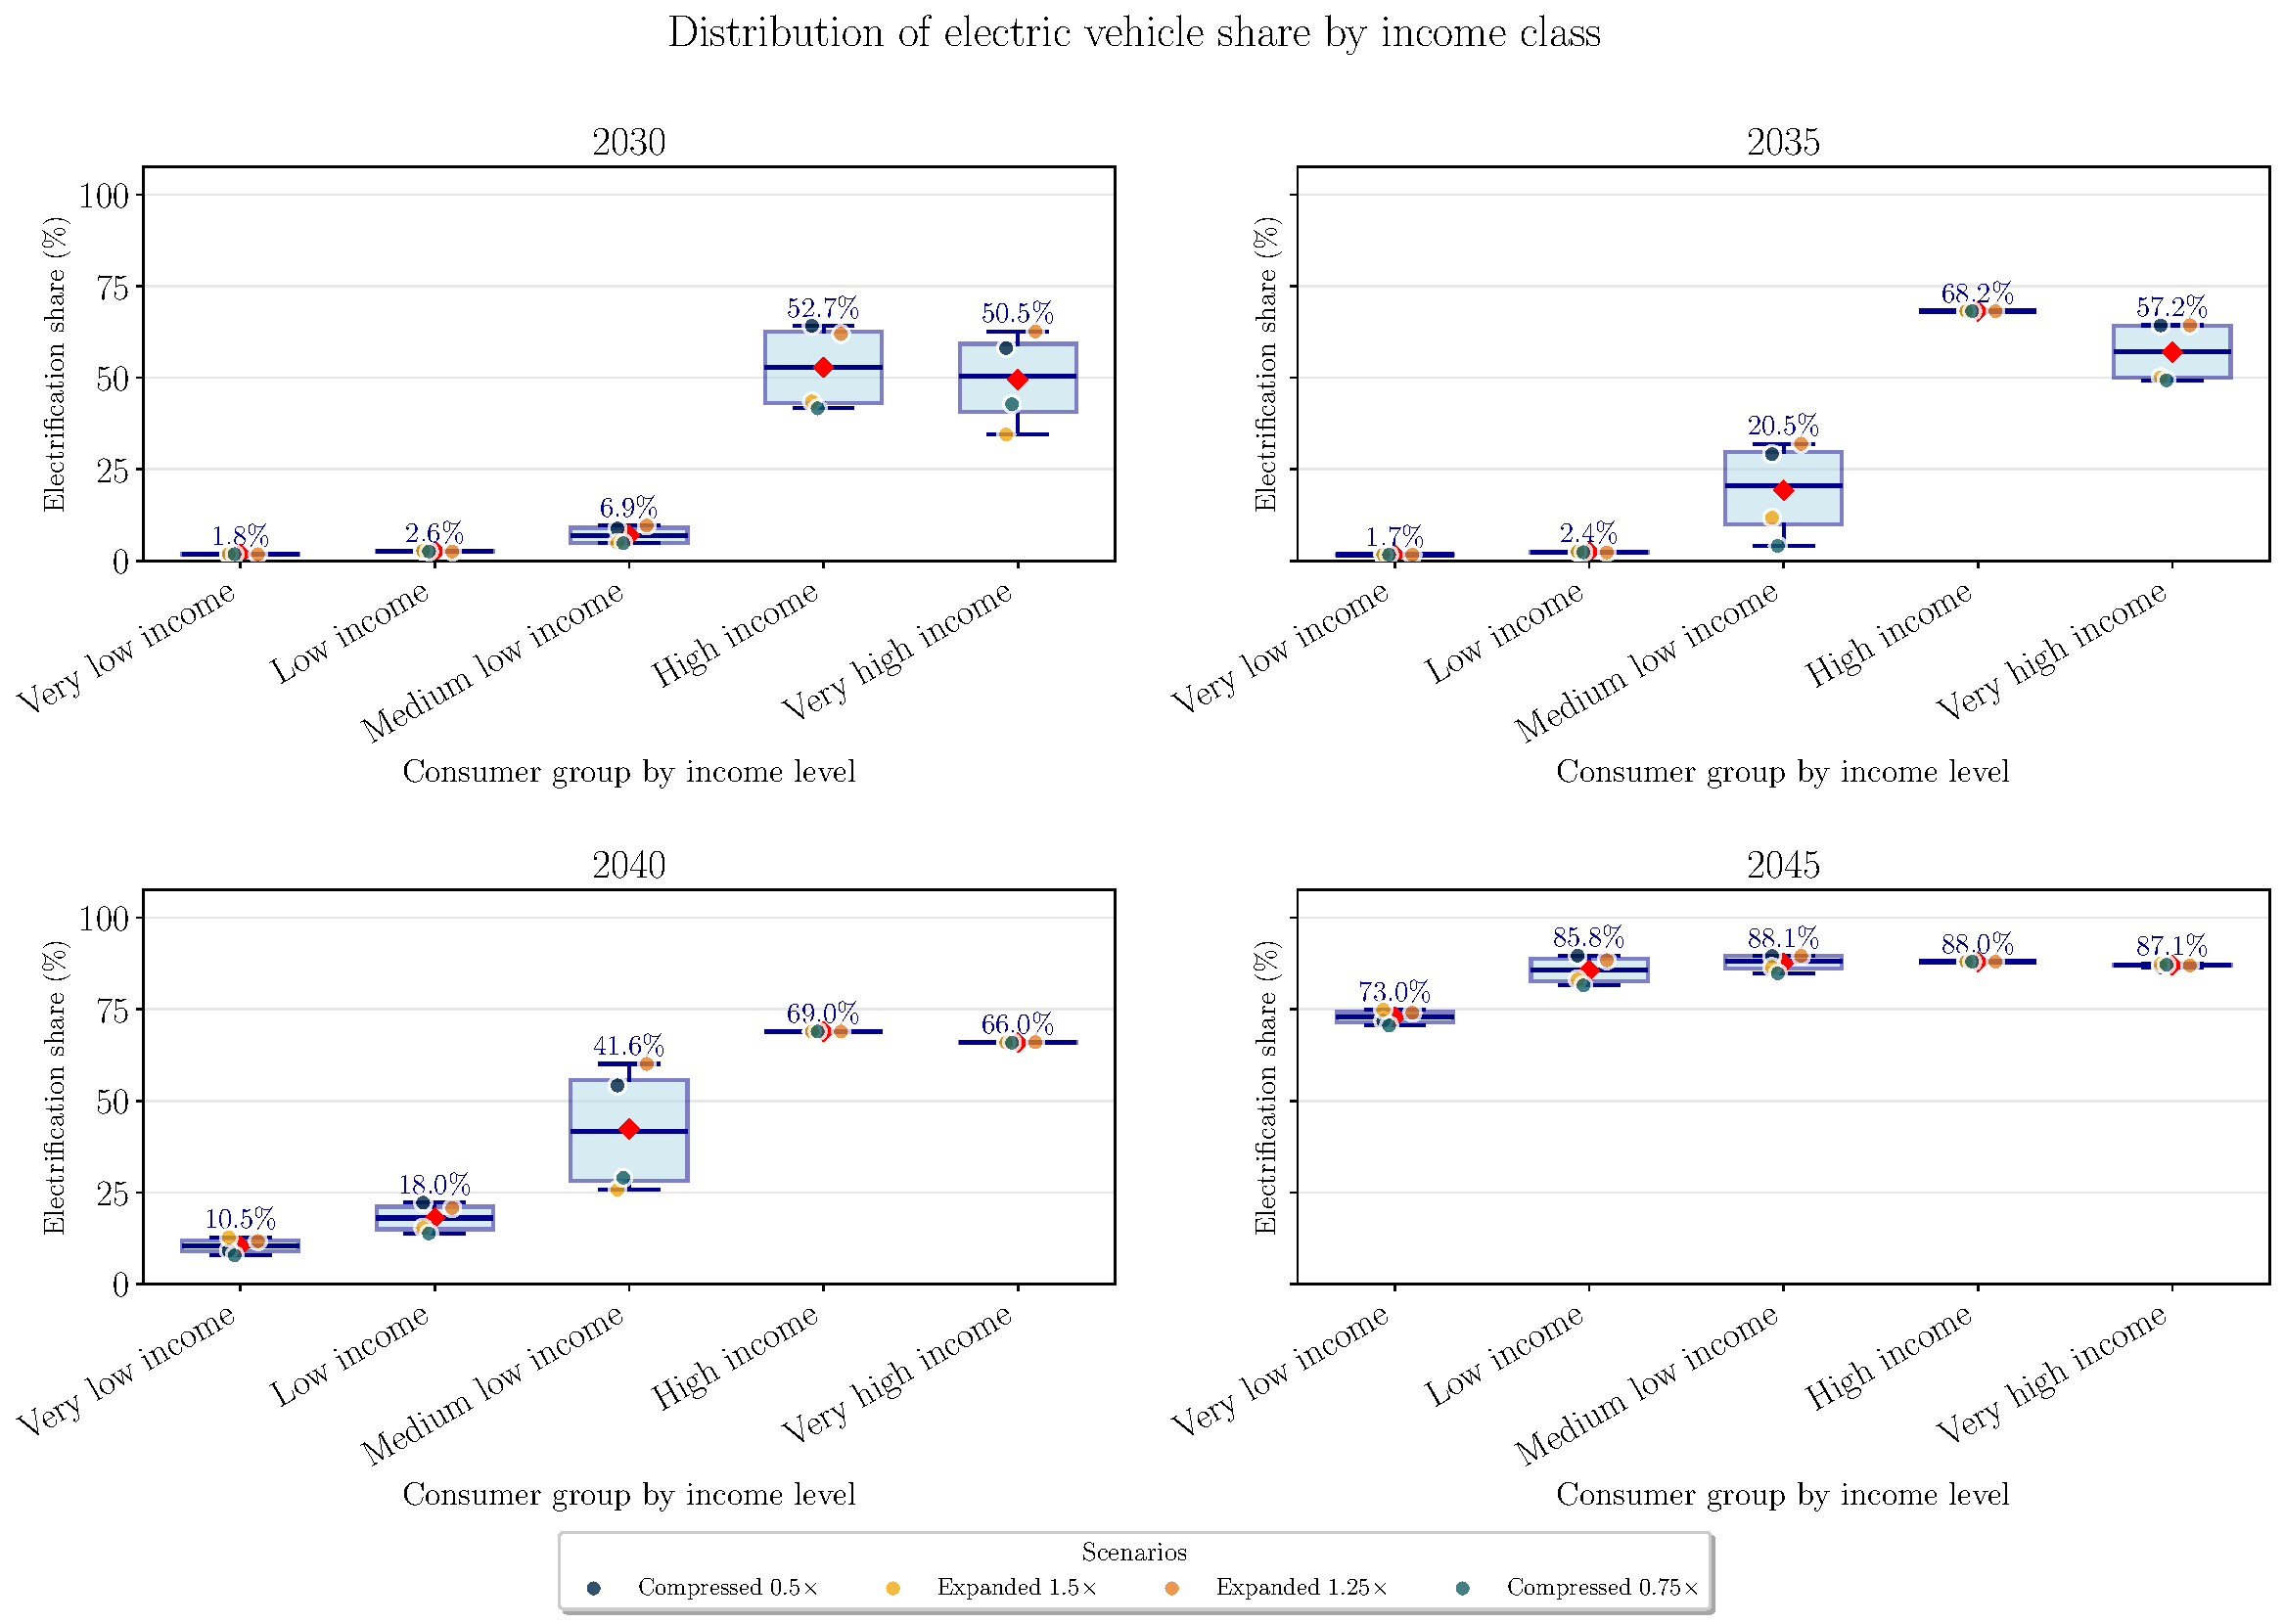
\includegraphics[width=\textwidth]{graphics/SA_boxplot_electric_vehicles_by_income.pdf} 
    \captionsetup{labelfont={color=authorblue}, textfont={color=authorblue}}
    \caption{Distribution of the development of electrification of passenger car fleet owned by consumer groups of different income levels observed during sensitivity analysis of different VoT parameterization.} \label{fig: VOT_bevs_2}
\end{figure} 

To address the reviewer’s suggestion regarding charging patterns, we next examine the differences in charged energy across charger types (see Figure \ref{fig: VOT_charging_pat_2}). We show a snapshot for 2050 displaying the usage patterns by the fully electrified fleet for a selection of four different VoT parameterizations. While there are no significant changes for consumer groups \textit{Very high income}, \textit{High income} and \textit{Medium low income}, the amount of fast charging capacity being used by the \textit{Very low income} and \textit{Low income} varies significantly between the VoT settings.

In Figure \ref{fig: VoT_fastcharg_2}, we take a closer look at the usage of fast charging capacities by \textit{Very low income} and \textit{Low income} consumer groups. In the cases where these groups have higher VoT, i.e. the VoT scenarios of \textit{Compressed 0.5x},  \textit{Compressed 0.75x} and \textit{Absolute +3}, the amount of fast charging is zero for the \textit{Low income} class.

\begin{figure}[H]
    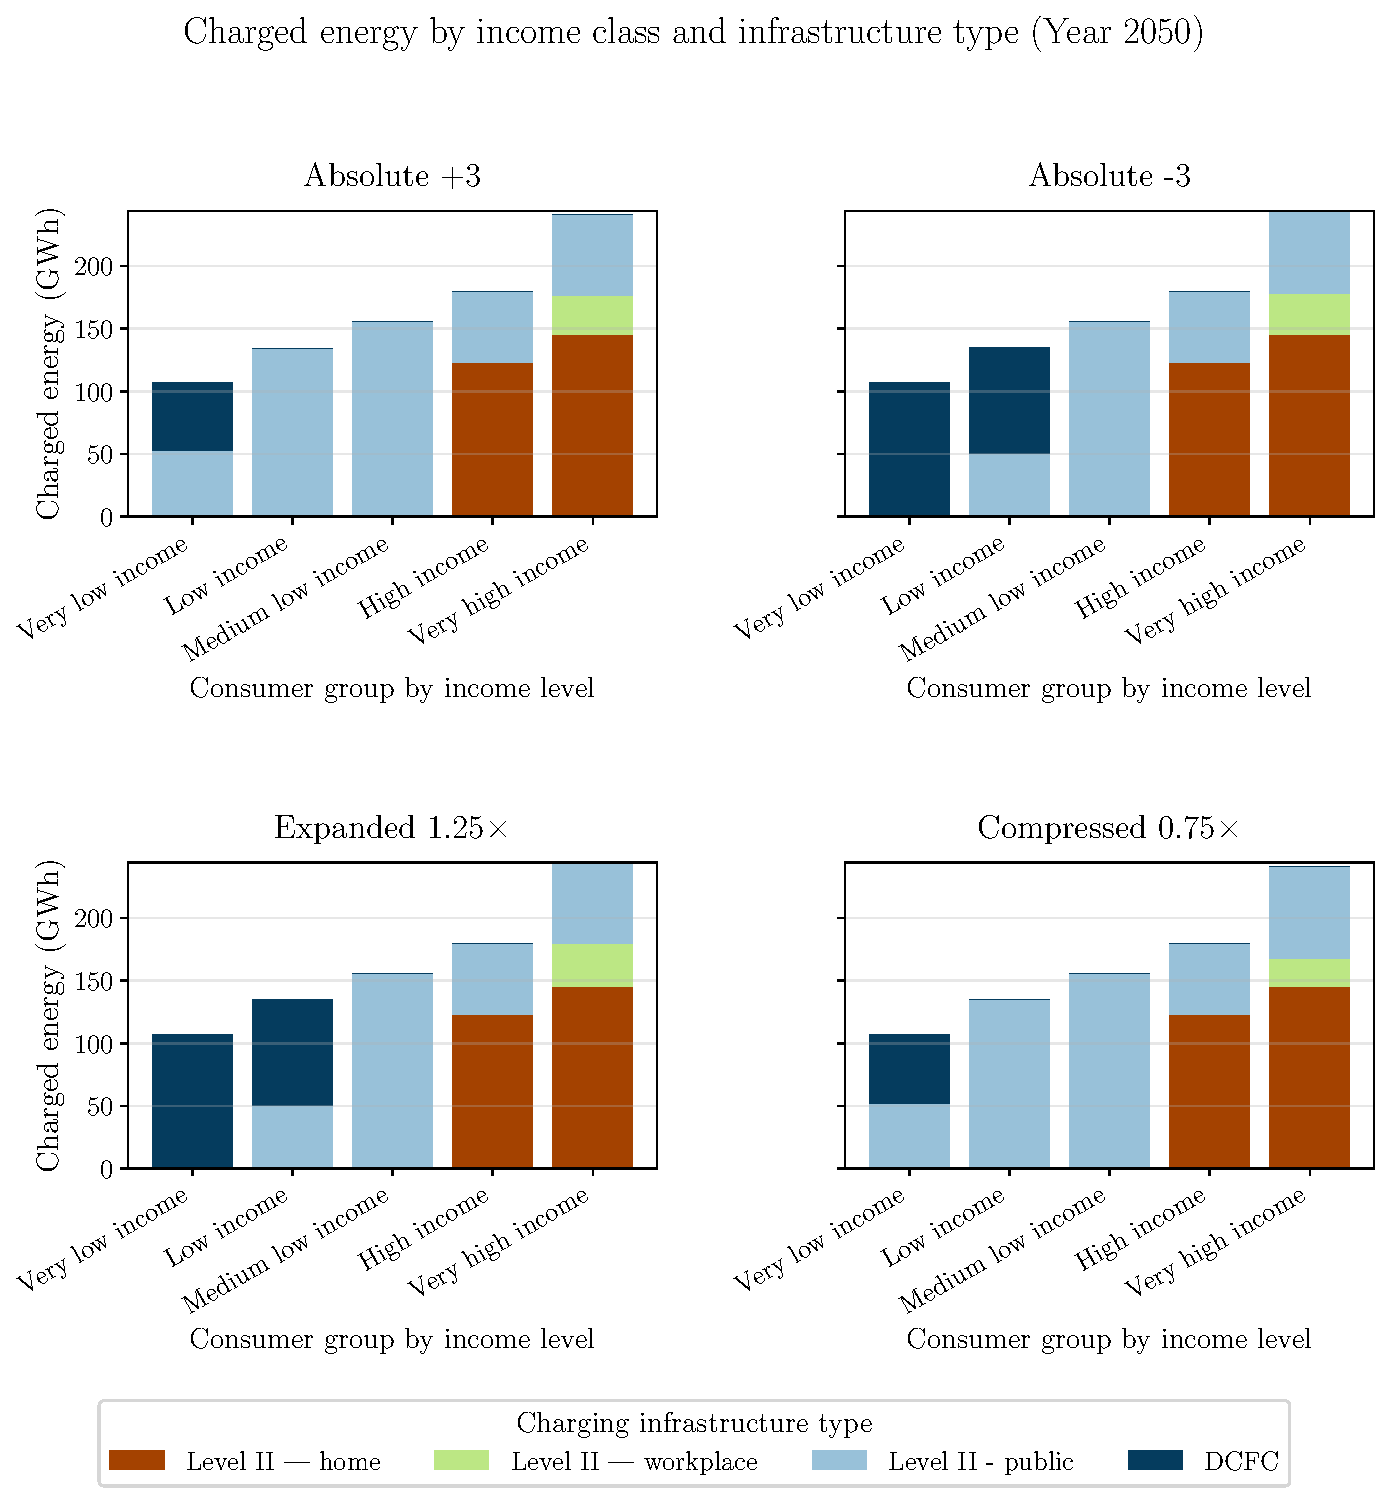
\includegraphics[width=0.7\textwidth]{graphics/SA_charged_energy_by_income_infrastructure.pdf} 
    \captionsetup{labelfont={color=authorblue}, textfont={color=authorblue}}
    \caption{Charged energy by charger type in 2050 for different VoT scenarios.} \label{fig: VOT_charging_pat_2}
\end{figure} 

\begin{figure}[H]
    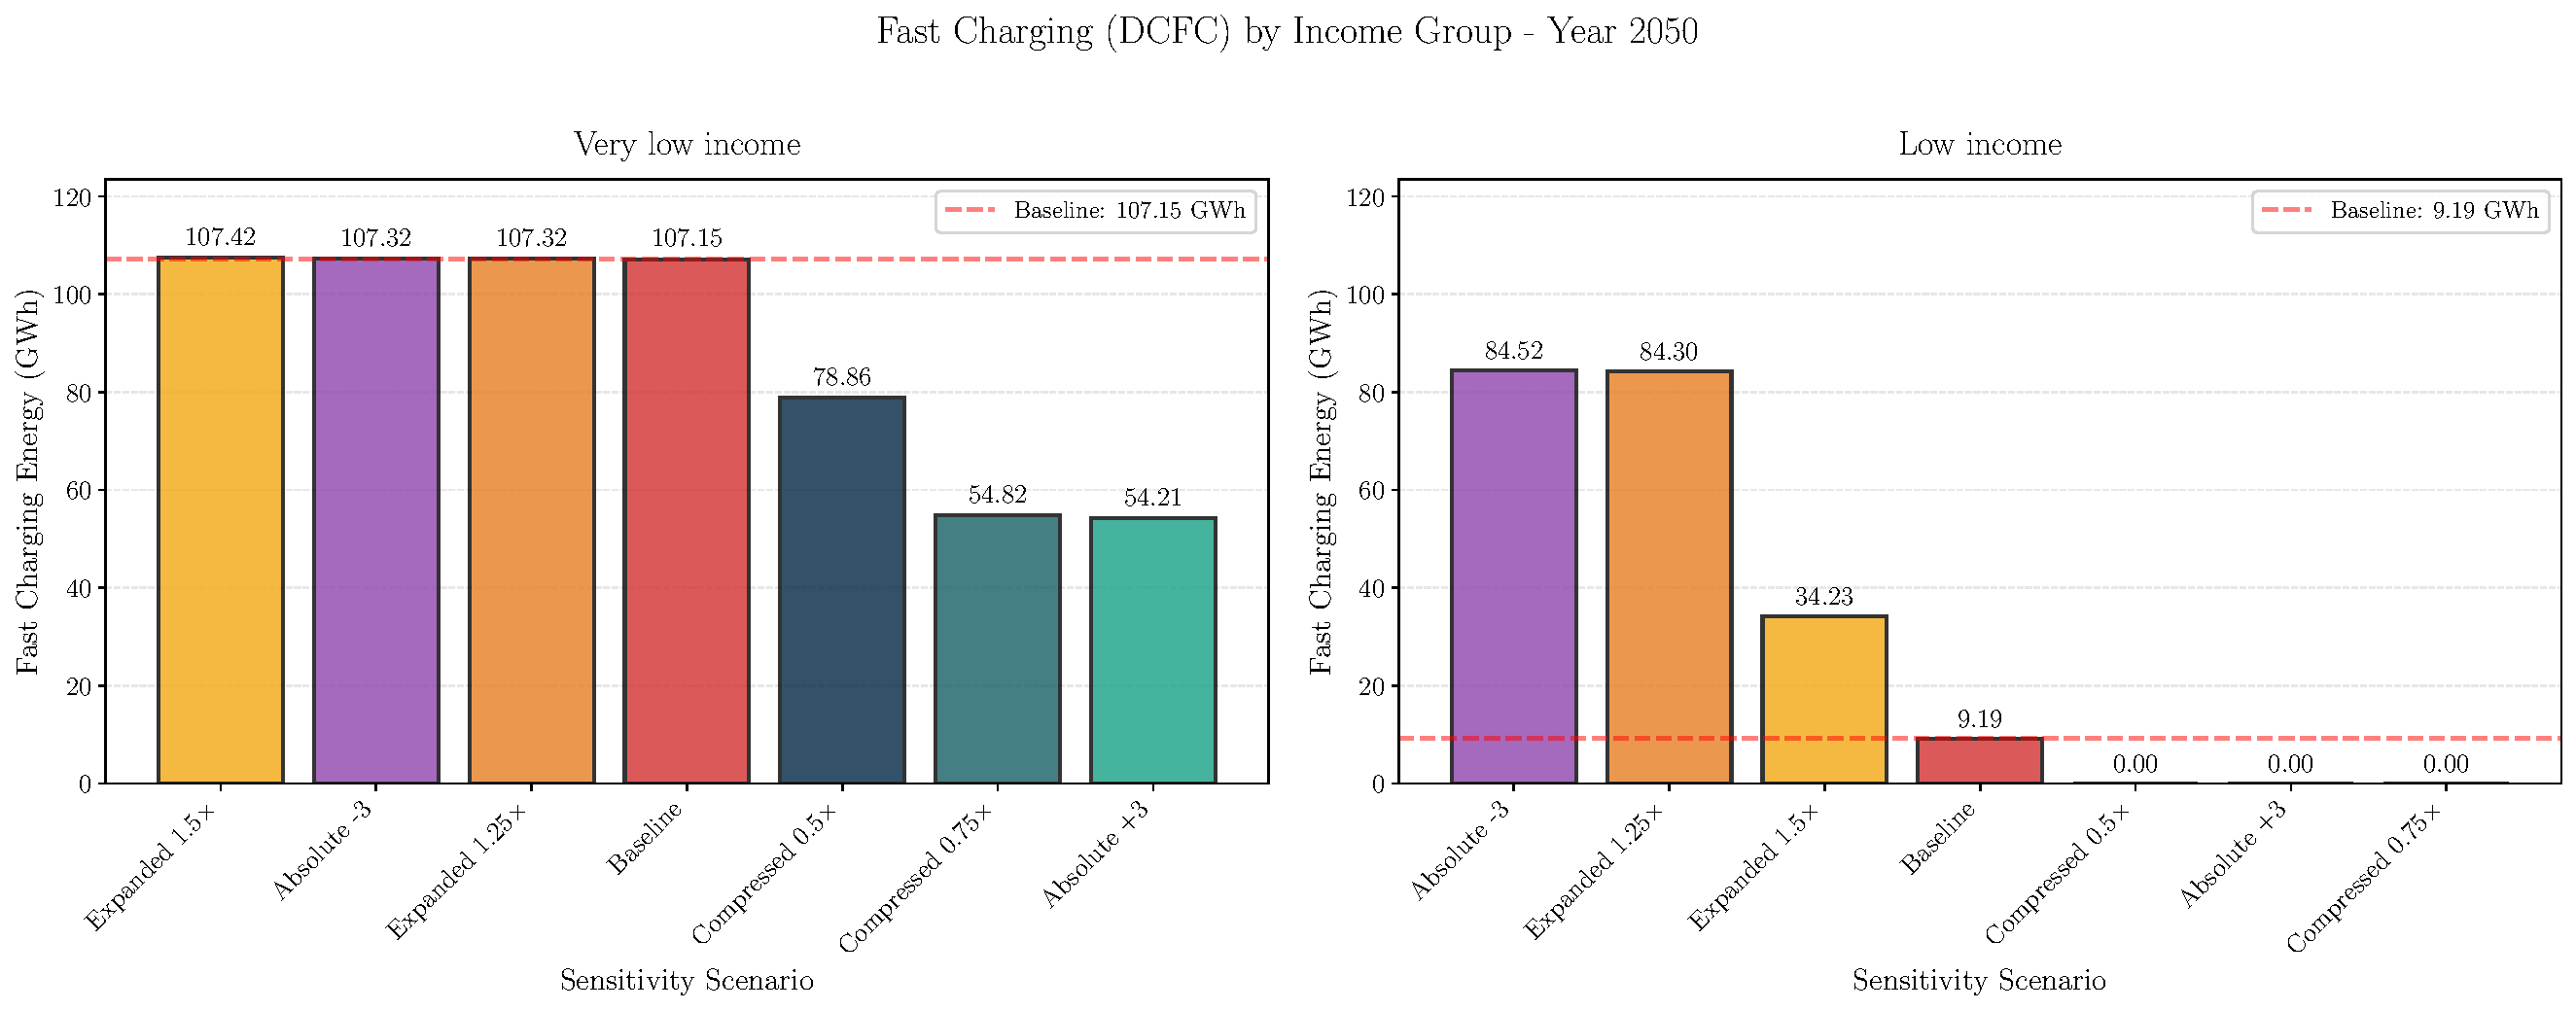
\includegraphics[width=0.9\textwidth]{graphics/SA_fast_charging_low_income_comparison.pdf} 
    \captionsetup{labelfont={color=authorblue}, textfont={color=authorblue}}
    \caption{Charged energy by fast chargers in 2050 for different VoT scenarios for consumer groups \textit{Very low income} (left) and \textit{Low income} (right).} \label{fig: VoT_fastcharg_2}
\end{figure} 

This observation is coherent with observations presented in the \textit{Results} section, in particular, Section 4.1. where we show differences of fast charger utilization through variation in levels of service induced by charging infrastructure densification. There, as well as in these VoT scenarios, we observe how the term $\mathrm{VoT} \times \mathrm{level~of~service}$ influences charger-type utilization across income groups.    

To provide a better understanding of the setting of the VoT parameter to the reader, we have now included this sensitivity analysis in the appendix of the manuscript (see Section B.2.).

\color{reviewergrey}
\subsubsection*{2. The baseline comparisons should be clearly labeled as omitting DCFC price premiums (compared to other charging modes) and queuing.}\\
\color{authorblue}
\noindent \textcolor{authorblue}{\textbf{Author's response:}} Thank you for the suggestion. We have included a footnote in the Results section (see Section 4.1) to emphasize this aspect for the interpretation of the results.

\color{reviewergrey}
\subsubsection*{3. The detour-time function should be more clearly documented with clear breakpoints/minima and a brief explanation of the underlying spatial heuristic, together with several sentences on the potential direction of bias so readers can interpret the results appropriately.}
\color{authorblue}

\noindent \textcolor{authorblue}{\textbf{Author's response:}} Thank you for this valuable feedback. Similar concerns have been raised by the other reviewers. We have added a clearer description of the piece-wise linearization in the appendix of the manuscript. The discretization of the detour fueling time function $g()$ has been conducted manually based on the educated guess of the authors, while keeping the number of break points sufficiently small to avoid computational complexity. We have conducted a sensitivity analysis with a coarser and finer resolution of the discretization procedure to understand the effect of it on our results. This is now clearly documented in the Appendix, Section A.3. 

Concerning the reviewer's comment on the spatial heuristics: We model the \textit{average} detouring time to the closest charging stations. As we model on NUTS-2 region level, we, on the one side, avoid computational complexity introduced by modeling the actual road network and vehicle movements, but, on the other side, have to make the assumption on the relative spatial relations between a BEV driver and the allocation of public charging sites. We introduce the assumption that charging sites would be spatially evenly distributed relative to BEV drivers. 

To better convey the underlying assumptions and the potential impacts on the results, we have extended the description of the detour fueling time function (Appendix Section A.3) and now describe the iimpacts of this assumption more clearly in the Discussion (Section 5.1.2).

Moreover, following a request from another reviewer, we now describe the results of a sensitivity analysis following a parameter that represents the road network efficiency in the detour fueling time function (see Appendix A.3).

\color{reviewergrey}
\subsubsection*{4. Reproducibility would benefit from a single supplemental "core assumptions" table. The table should list units and sources for the income-class parameters (e.g., value of time, budgets, etc.), utilization caps and power levels by charger type, public-charging detour parameters, density scenarios, etc. Concentrating these inputs in one place will make the study easier to cite and extend.}
\color{authorblue}
\noindent \textcolor{authorblue}{\textbf{Author's response:}} 

Thank you for noting this aspect. In the course of updating the manuscript during this review, we have improved the detail in describing the methodology and assumptions, which has also benefited reproducibility. We chose not to include a single summary table, as the parameters and data are too diverse in structure and dimension to present in one readable table. For full reproducibility, we have published the code and input data on GitHub (\url{https://github.com/antoniamgolab/iDesignRES_transcompmodel}).

\color{reviewergrey}
\newpage
\fancyhead[L]{\textit{Response to Reviewer \#3}}
\section*{Reviewer \#3}
\textbf{This paper explores two important and timely questions in EV infrastructure planning: (RQ1) how different roll-out strategies affect various income groups, and (RQ2) how infrastructure deployment generates cross-regional spillover effects. The authors present a well-designed techno-economic optimization framework to tackle these interconnected issues. Its contributions, particularly the modeling of "fueling detour time" and spatial spillovers, offer valuable insights to the field. However, the strength of the paper's conclusions is undermined by major issues concerning the foundational data and key methodological assumptions. As the reliability of model outputs depends on input quality, the validity and transferability of the core data warrant closer scrutiny. Substantial revisions are required to solidify the paper's methodological base and ensure that its findings are credible and generalizable.}
\\ 
\color{authorblue}\noindent \textcolor{authorblue}{\textbf{Author's response:}} Thank you for your time spent on reviewing our manuscript. In order to strengthen the paper's conclusion, we have added results of sensitivity analyses on crucial parameters to the appendix of the manuscript. To offer better insights into the assumptions of data and their potential impact, we have revised sections describing the Methodology (Section 3) and the Discussion (Section 5). In the following we address each of this review's concerns and described the corresponding revisions to our manuscript.
\\
\\
\color{reviewergrey}
\textbf{The model is built on a "patchwork" of non-local proxy data, with several key assumptions left insufficiently justified. To be fair, obtaining comprehensive and credible data for such analyses is inherently challenging, and researchers often have to make the most of what is available. However, this makes it even more important to ensure that these data are used transparently, appropriately, and with clear acknowledgment of their limitations.} \\ 
\color{reviewergrey}
\subsubsection*{1. Foundational Travel Demand (O-D) Data (Section 3.3.1 and Appendix A.2.1)}
\setcounter{reviewcounter}{0} % set the counter of the comments to 
\textbf{a. The model is based on the ETISplus database from 2010. Using travel patterns from 15 years ago to forecast adoption out to 2050 is a significant concern. Travel behavior has changed profoundly due to several factors (e.g., remote work, ride-sharing, gig economy) that are not captured in 2010 data. Simply scaling this old data by historic GDP growth (as mentioned in Sec 3.3.1) does not account for fundamental shifts in why and where people travel.}\\\\
\color{authorblue}
\noindent \textcolor{authorblue}{\textbf{Author's response:}}  Thank you for highlighting this important assumption made in our work. We are using data from ETISplus as the basis of our work due to the lack of a sufficient alternative database that indicates the amount of commuting traffic between the regions. To compensate for the fact that this data describes trip data for the year 2010, we scale the data using the GDP growth since then as an indicator. It is a common approach in the literature to use GDP growth for extrapolating the growth of passenger road transport demand \citep{EDELENBOSCH2017281, thomsen2024projecting}. We are convinced that there is a limited value of adding a sensitivity analysis on the absolute numbers of the person-trips and decided to focus on conducting sensitivity analyses on more impactful model parameters during this revision round. 
As the reviewer suggested, we have now included a short discussion on this limitation in the \textit{Discussion} section (Section 5.2). \\ \\
\color{reviewergrey}
\textbf{b. The paper notes that route lengths for internal trips (within a NUTS-3 region) were missing. To fill this gap, the authors imported data from a 2016 Austrian mobility survey, applying data from Vienna, Austria to Basque urban areas (Table 3). This proxy data is a major source of uncertainty. The authors must provide a robust justification for this transferability. For this assumption to be valid, they would need to demonstrate, for example, that the urban/rural geographies and, most importantly, the passenger car mode shares for these trip types are comparable between the Austrian case study and the Basque Country. Without this supporting evidence, the input data for all local trips is highly questionable.} \\\\
\color{authorblue}
\noindent \textcolor{authorblue}{\textbf{Author's response:}} We acknowledge the uncertainty introduced by using Austrian trip length data. However, we argue this assumption primarily affects absolute values (fleet sizes, infrastructure capacities) rather than the relative patterns across income classes that form our core findings. This is because trip lengths enter the model uniformly across all income groups—the differentiation between income classes stems from VoT, budgets, and home charging access, not from trip distances. Therefore, while alternative trip length data would shift absolute magnitudes, the relative differences in charging behavior and adoption timing across income classes would be preserved. h broadly comparable urban structures, making this proxy more appropriate than alternatives from non-European contexts. Given this, there are indicators for travel behavior that have values in similar range between the Basque Country and Austria. The Basque country is among the regions with highest GDP in Spain [Basque country: 116 in 2023; Austria: 118 in 2023; Source: \citep{eustat_gdp_ppp_2025}]. The article \citep{eurostat_commuting_2019} identifies similar commuting times for Spain and Austria (Spain: 25min; Austria: 24min in 2019). \\ \\

\color{reviewergrey}
\textbf{c. The paper's primary research question (RQ1) is about the impact on different income classes. However, Appendix A.2.2 explicitly states: "As there is no income-class-related information in the OD data set, the assumption is that these [trip frequencies] are constant among all income classes." This assumption fundamentally undermines RQ, as this assumes that they all travel identically.}\\\\
\color{authorblue}
\noindent \textcolor{authorblue}{\textbf{Author's response:}} 
We thank the reviewer for this important concern. Our analysis does not assume identical travel behavior across income classes. While trip frequencies are held constant among vehicle owners, we differentiate income classes through the parameters that literature identifies as primary determinants of charging behavior:
\begin{itemize}
    \item Motorization rates — lower-income households have systematically lower car ownership
    \item Monetary budgets — income-specific constraints on vehicle purchases
    \item Value of Time (VoT) — determining trade-offs between charging time and other costs
    \item Home charging access — differentiated by income-specific home ownership rates
\end{itemize}

Empirical research indicates that income primarily affects the degree of motorization rather than trip patterns among car owners \citep{tikoudis2024oecd246, CHATTERTON201830}. Our model captures this primary source of differentiation.
Our VoT sensitivity analysis (Appendix B.2) confirms these mechanisms produce substantial behavioral variation: BEV adoption spreads up to 45 percentage points for Medium-low income groups, and fast charging usage varies from 0 to 84 GWh for low-income consumers depending on VoT specification. This demonstrates that our income differentiation approach generates meaningful and policy-relevant variation across income classes.
\textbf{We have revised the Methodology section (Section 3.1.1) to explicitly describe our income differentiation approach and removed the potentially misleading statement from Appendix A.2.2.}

\color{reviewergrey}
\subsubsection*{2. Non-Local Value of Time (VoT) - The paper adopts VoT values from a 2018 Danish case study (Tattini et al., 2018), citing a lack of local data. However, VoT is highly specific to a region's local economy, wage structures, and cost of living. It is not a value that can be easily transferred from Denmark to Spain with just "purchase power" adjustment. This proxy directly influences the model's cost-benefit trade-offs and likely explains counter-intuitive results (e.g., the "Very low income" group's high use of DCFC in Fig. 9)} \\
\color{authorblue} \noindent \textcolor{authorblue}{\textbf{Author's response:}} We agree that this assumption is challenging. This issue has been raised by all reviewers in this review process. 

Our scaling approach using the \textit{Purchase Power Parity} value is in line with the finding of the study by \citet{WARDMAN201693}. The authors address the transferability of VoT values between past conducted studies focusing on different modes, purposes of trips and countries quantifying the VoT. They conduct exploratory analysis and find that the biggest impact across countries and mode types are the income levels and the purchase power. To gain understanding in the impact of the parameterization of the VoT values, we have conducted a sensitivity analysis that aims to assess the impact of the absolute level of the VoT values and on the relative values between the different income class levels. The results of this sensitivity analysis are included in the revised version of the manuscript (see Section B.2).

In the design of the sensitivity analysis, we tackle two aspects: Different absolute values and relative differences between the income classes. The following two figures display the tested VoT scenarios:

\begin{figure}[H]
    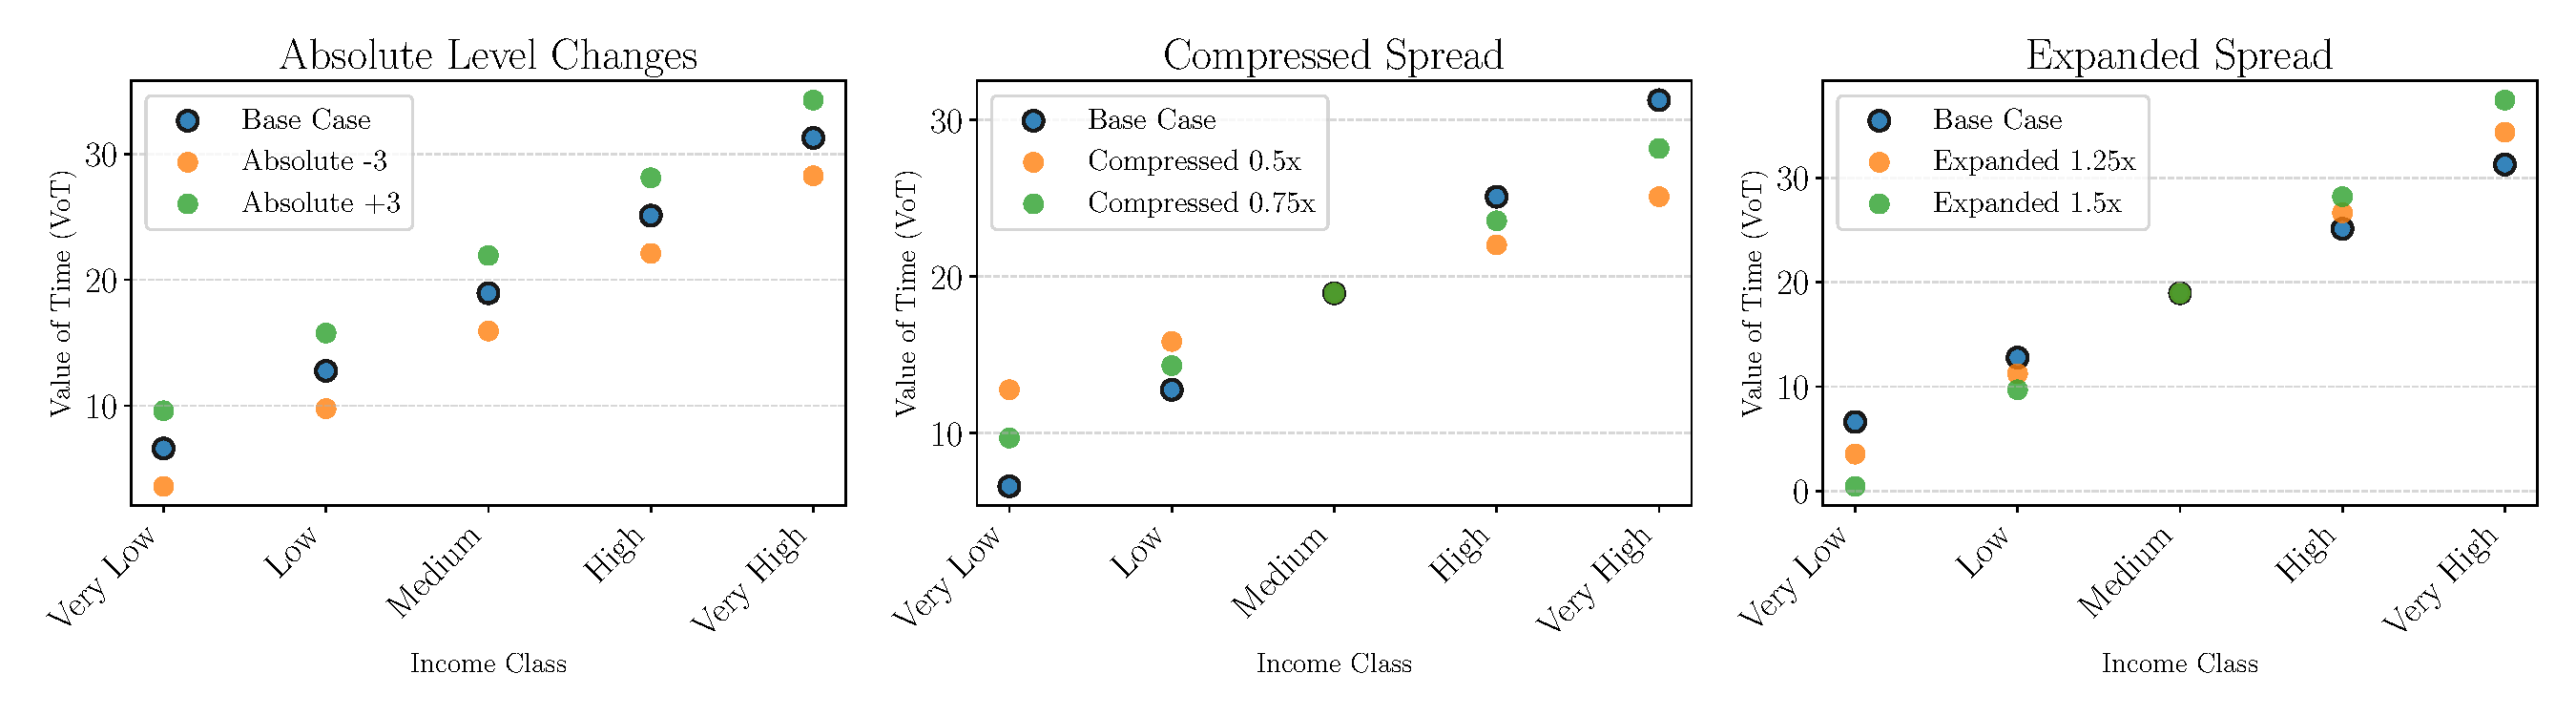
\includegraphics[width=\textwidth]{graphics/sensitivity_analysis_vot.pdf} 
        \captionsetup{labelfont={color=authorblue}, textfont={color=authorblue}}

    \caption{The \textit{Base Case} displays the assumed VoT values for the Basque country. \textit{Left:} VoT values for absolute increase and decrease of the value of time. \textit{Center:} Two cases of smaller relative changes between the VoT per income class. \textit{Right:} Higher relative changes between the VoT per income class.} \label{fig: VoT_tesing_3}
\end{figure} 

The tested shifts of absolute levels are $\pm 3$ which equal approximately absolute differences between the VoT values between inter-city vs. urban car trips in Spain \citep{WARDMAN201693}. As the \textit{Base Case} for this sensitivity analysis we use the densification scenario of $n^{\mathrm{points per site}} = 10$.

Figure \ref{fig: VOT_bevs_3} displays the distribution of electrification shares by the consumer groups for years 2030, 2035, 2040 and 2045. Overall, no significant outliers are shown. The highest impact of the VoT parameter is visible for the consumer group \textit{Medium low income}. This particularly becomes visible for the years 2035 and 2040, where the spread is up to around 45\%. The extreme values here are particularly given by \textit{Expanded 1.25x} and \textit{Expanded 1.5x}, and \textit{Compressed 0.5x} and  \textit{Compressed 0.75x}. The average VoT of these VoT scenarios are the same. Therefore, there is a particular sensitivity to the relative differences between the income-class specific VoT parameters in the adoption of BEVs. 

\begin{figure}[H]
    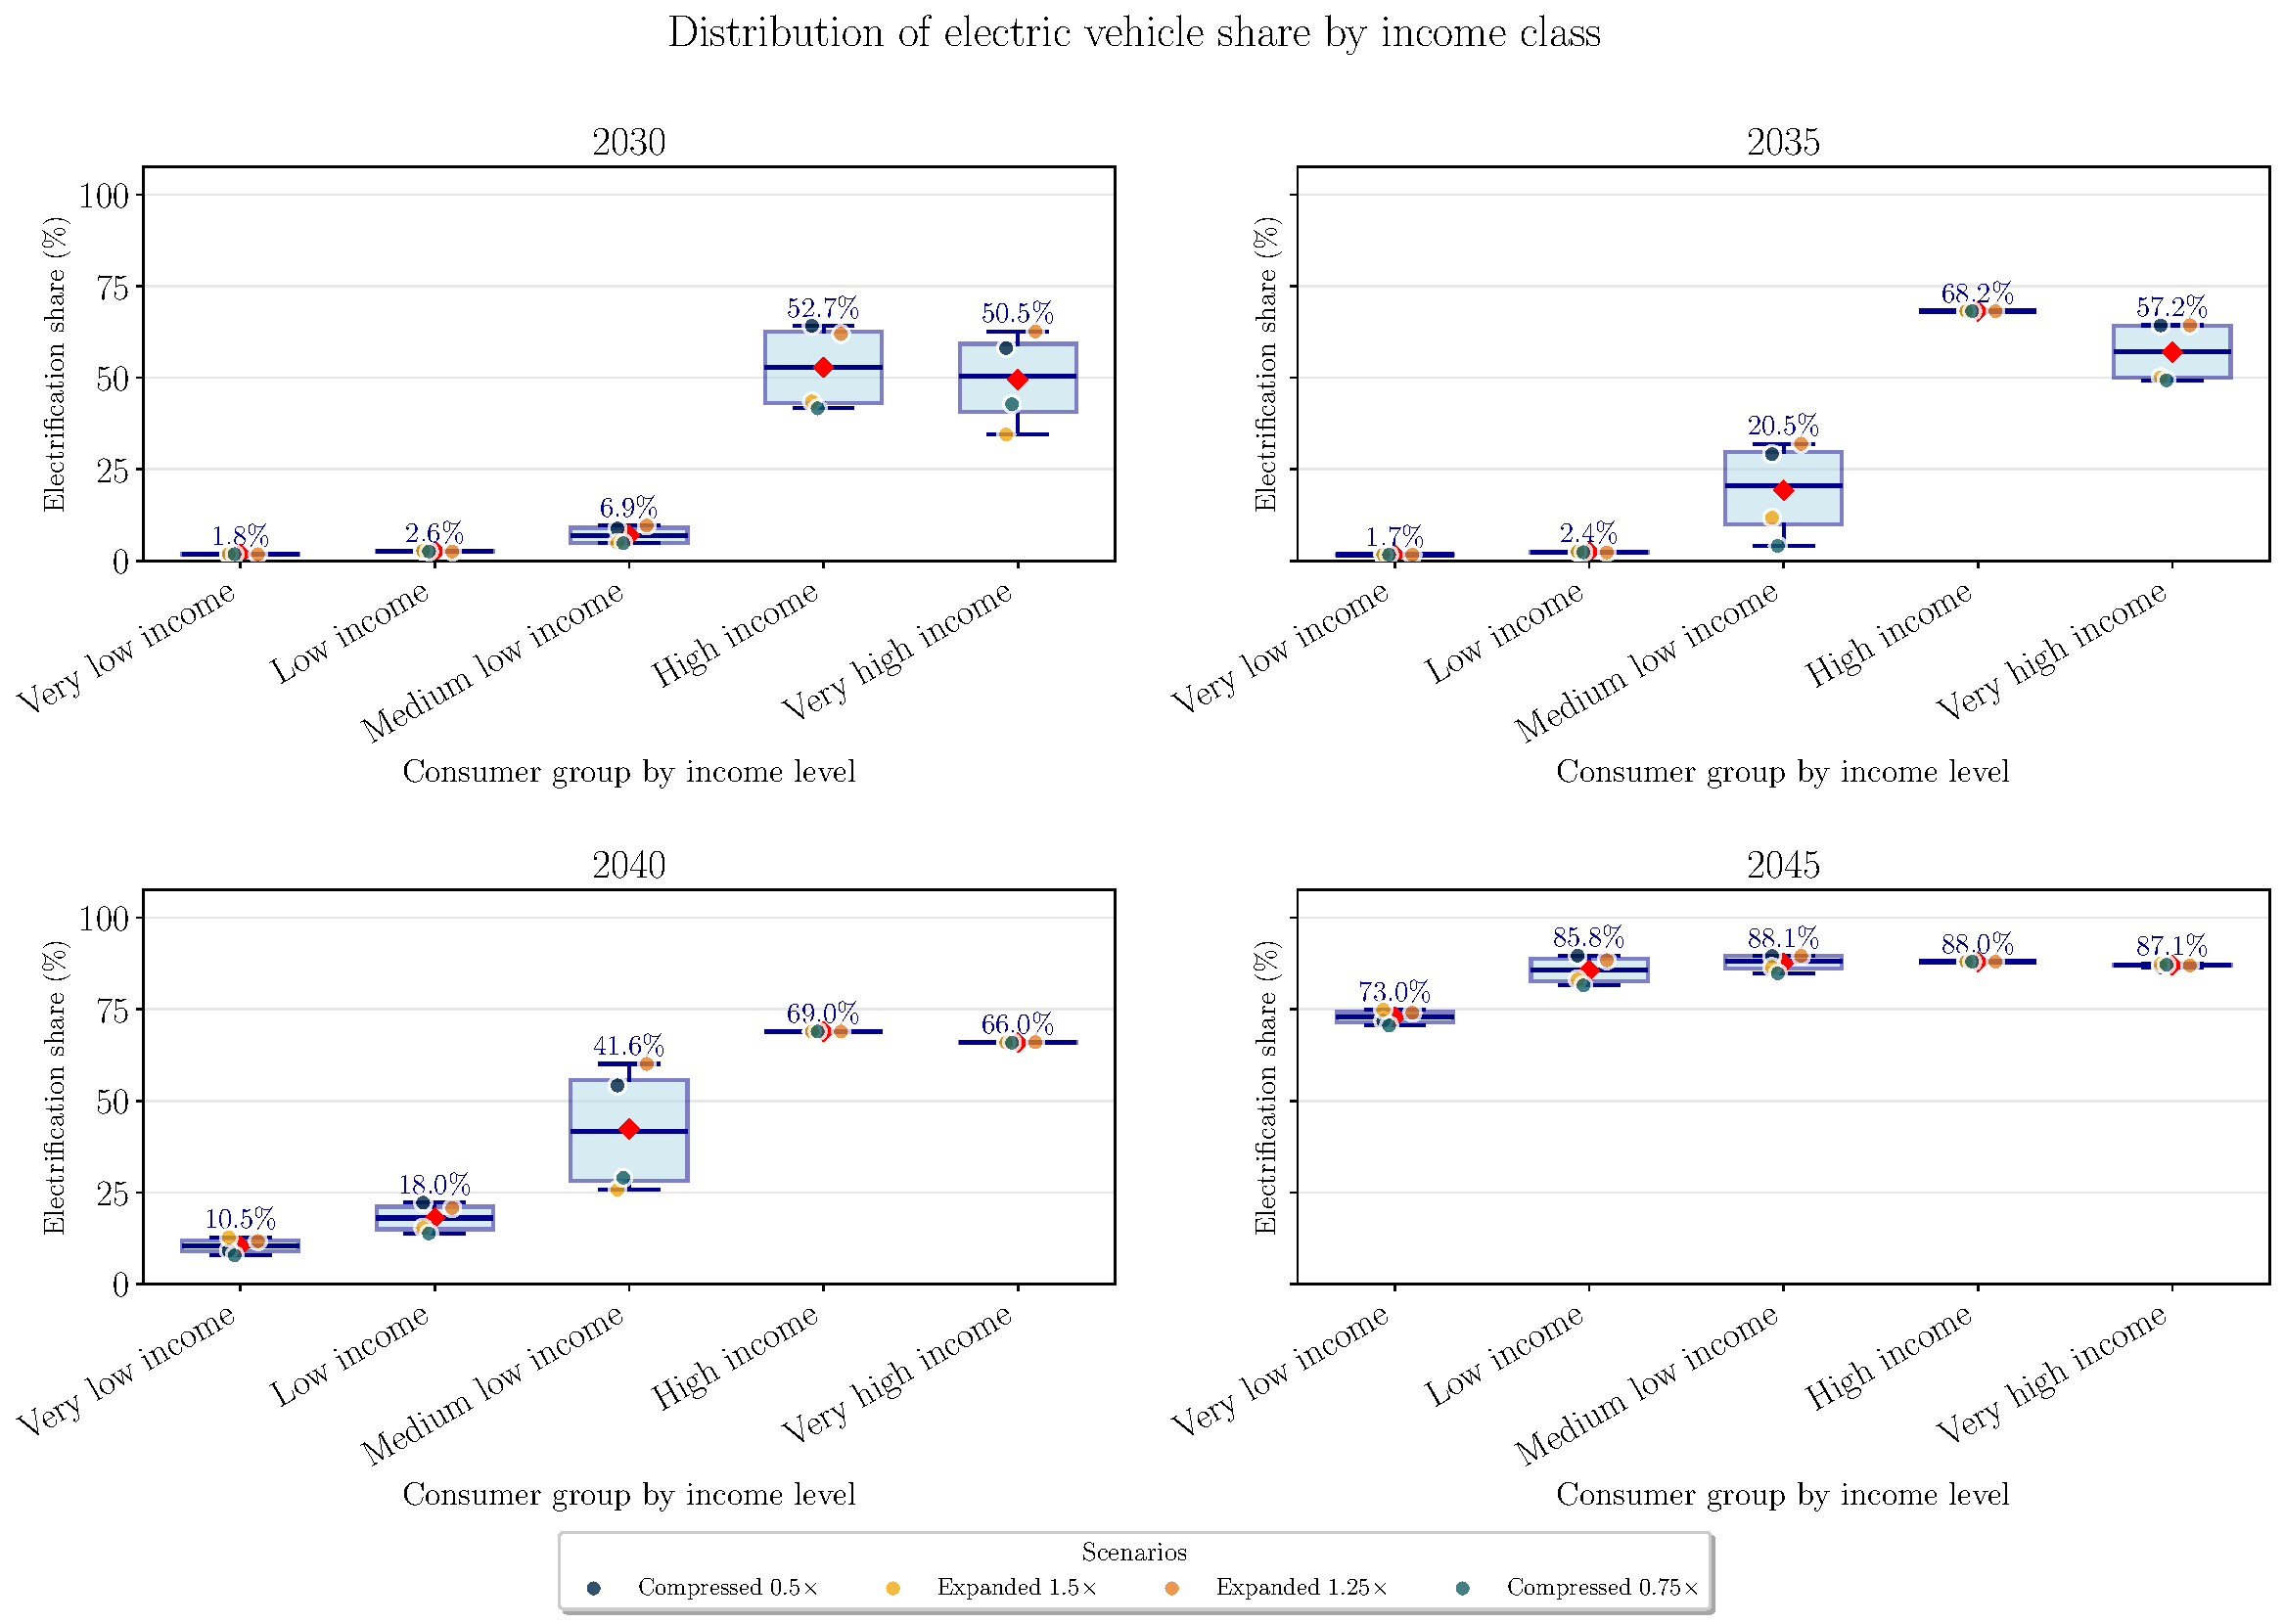
\includegraphics[width=\textwidth]{graphics/SA_boxplot_electric_vehicles_by_income.pdf} 
        \captionsetup{labelfont={color=authorblue}, textfont={color=authorblue}}
    \caption{Distribution of the development of electrification of passenger car fleet owner by consumer groups of different income levels observed during sensitivity analysis of different VoT parameterization.} \label{fig: VOT_bevs_3}
\end{figure} 

To address the reviewer’s suggestion regarding charging patterns, we next examine the differences in charged energy across charger types (see Figure \ref{fig: VOT_charging_pat_4}). We show a snapshot for 2050 displaying the usage patterns by the 100\% electrified fleet for a selection of four different VoT parameterizations. While there are no significant changes for consumer groups \textit{Very high income}, \textit{High income} and \textit{Medium low income}, the amount of fast charging capacity being used by the \textit{Very low income} and \textit{Low income} varies significantly between the VoT settings.

In Figure \ref{fig: VoT_fastcharg_4}, we take a closer look at the usage of fast charging capacities by  \textit{Very low income} and \textit{Low income} consumer groups. In the cases where these groups have higher VoT, i.e. the VoT scenarios of \textit{Compressed 0.5x},  \textit{Compressed 0.75x} and \textit{Absolute +3}, the amount of fast charging is zero for the \textit{Low income} class.

\begin{figure}[H]
    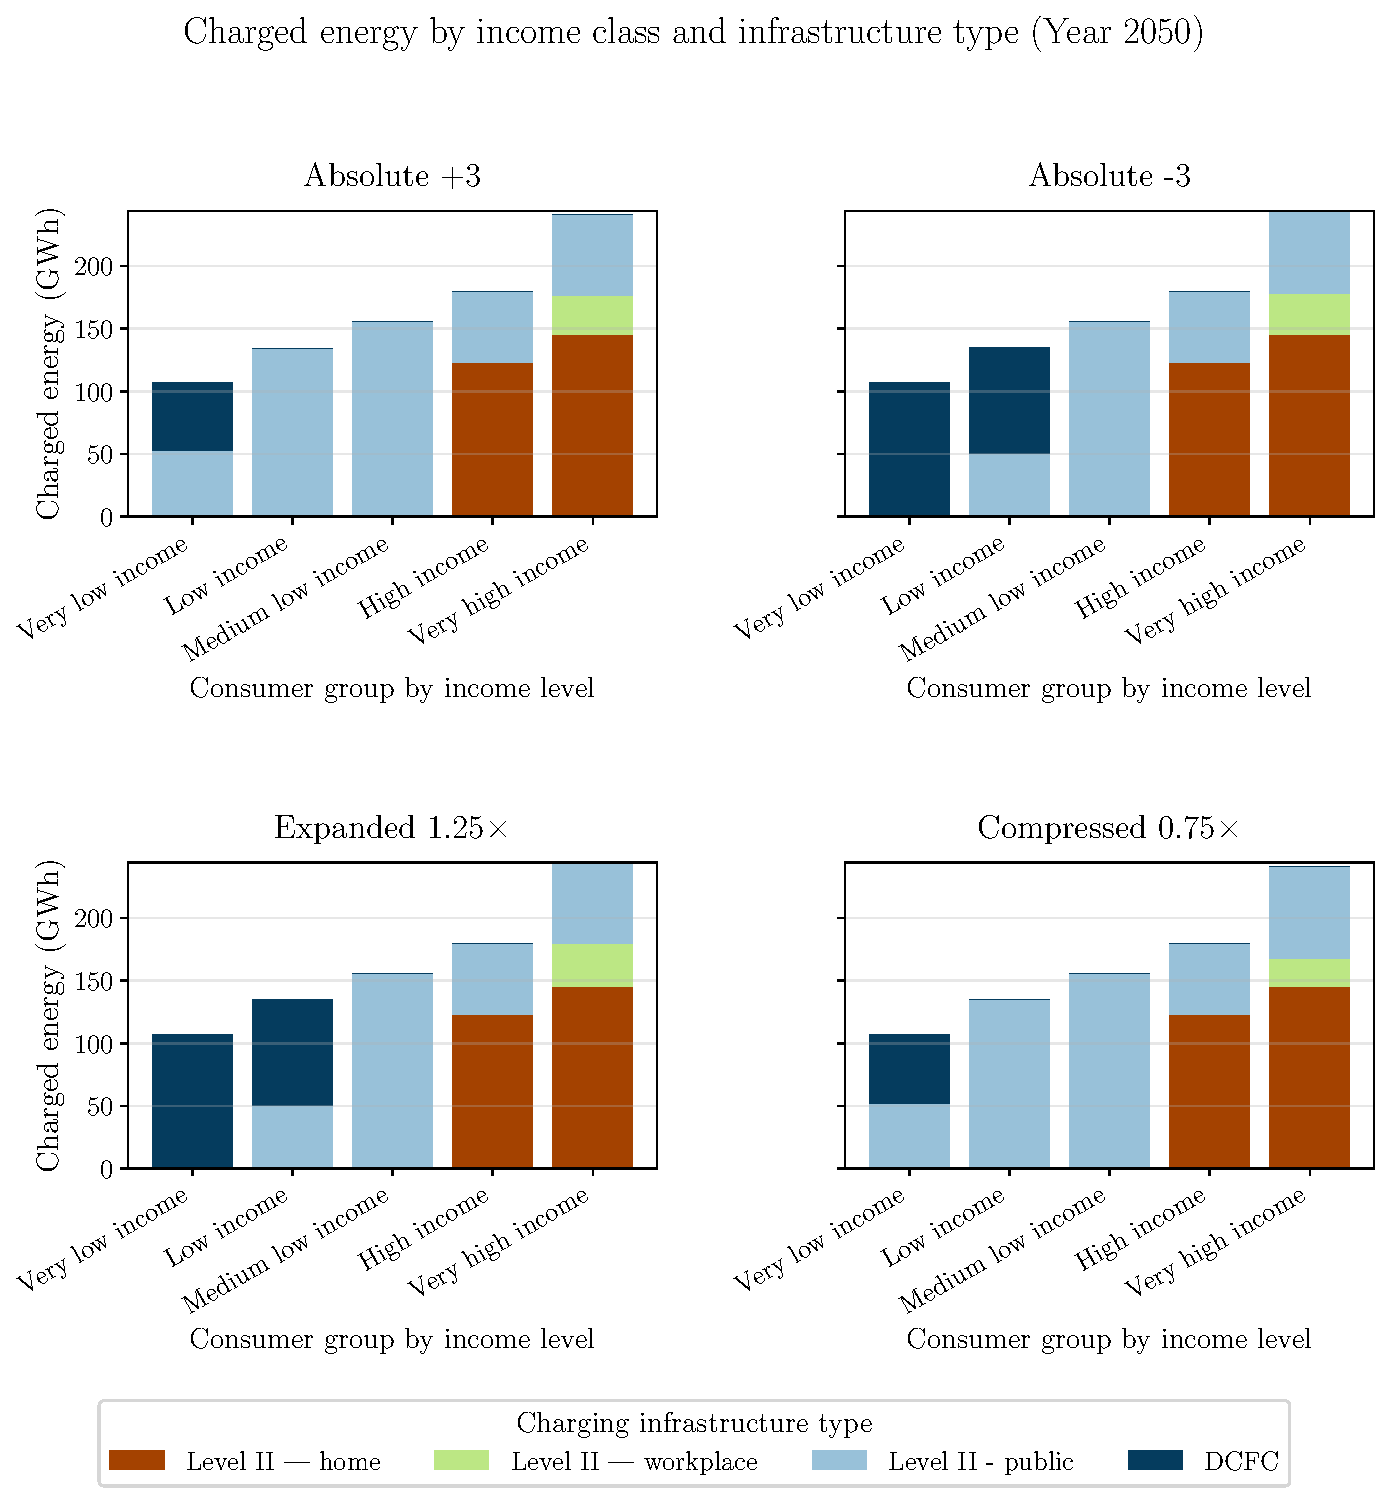
\includegraphics[width=0.7\textwidth]{graphics/SA_charged_energy_by_income_infrastructure.pdf}
    \captionsetup{labelfont={color=authorblue}, textfont={color=authorblue}}
    \caption{Charged energy by charger type in 2050 for different VoT scenarios.} \label{fig: VOT_charging_pat_4}
\end{figure} 

\begin{figure}[H]
    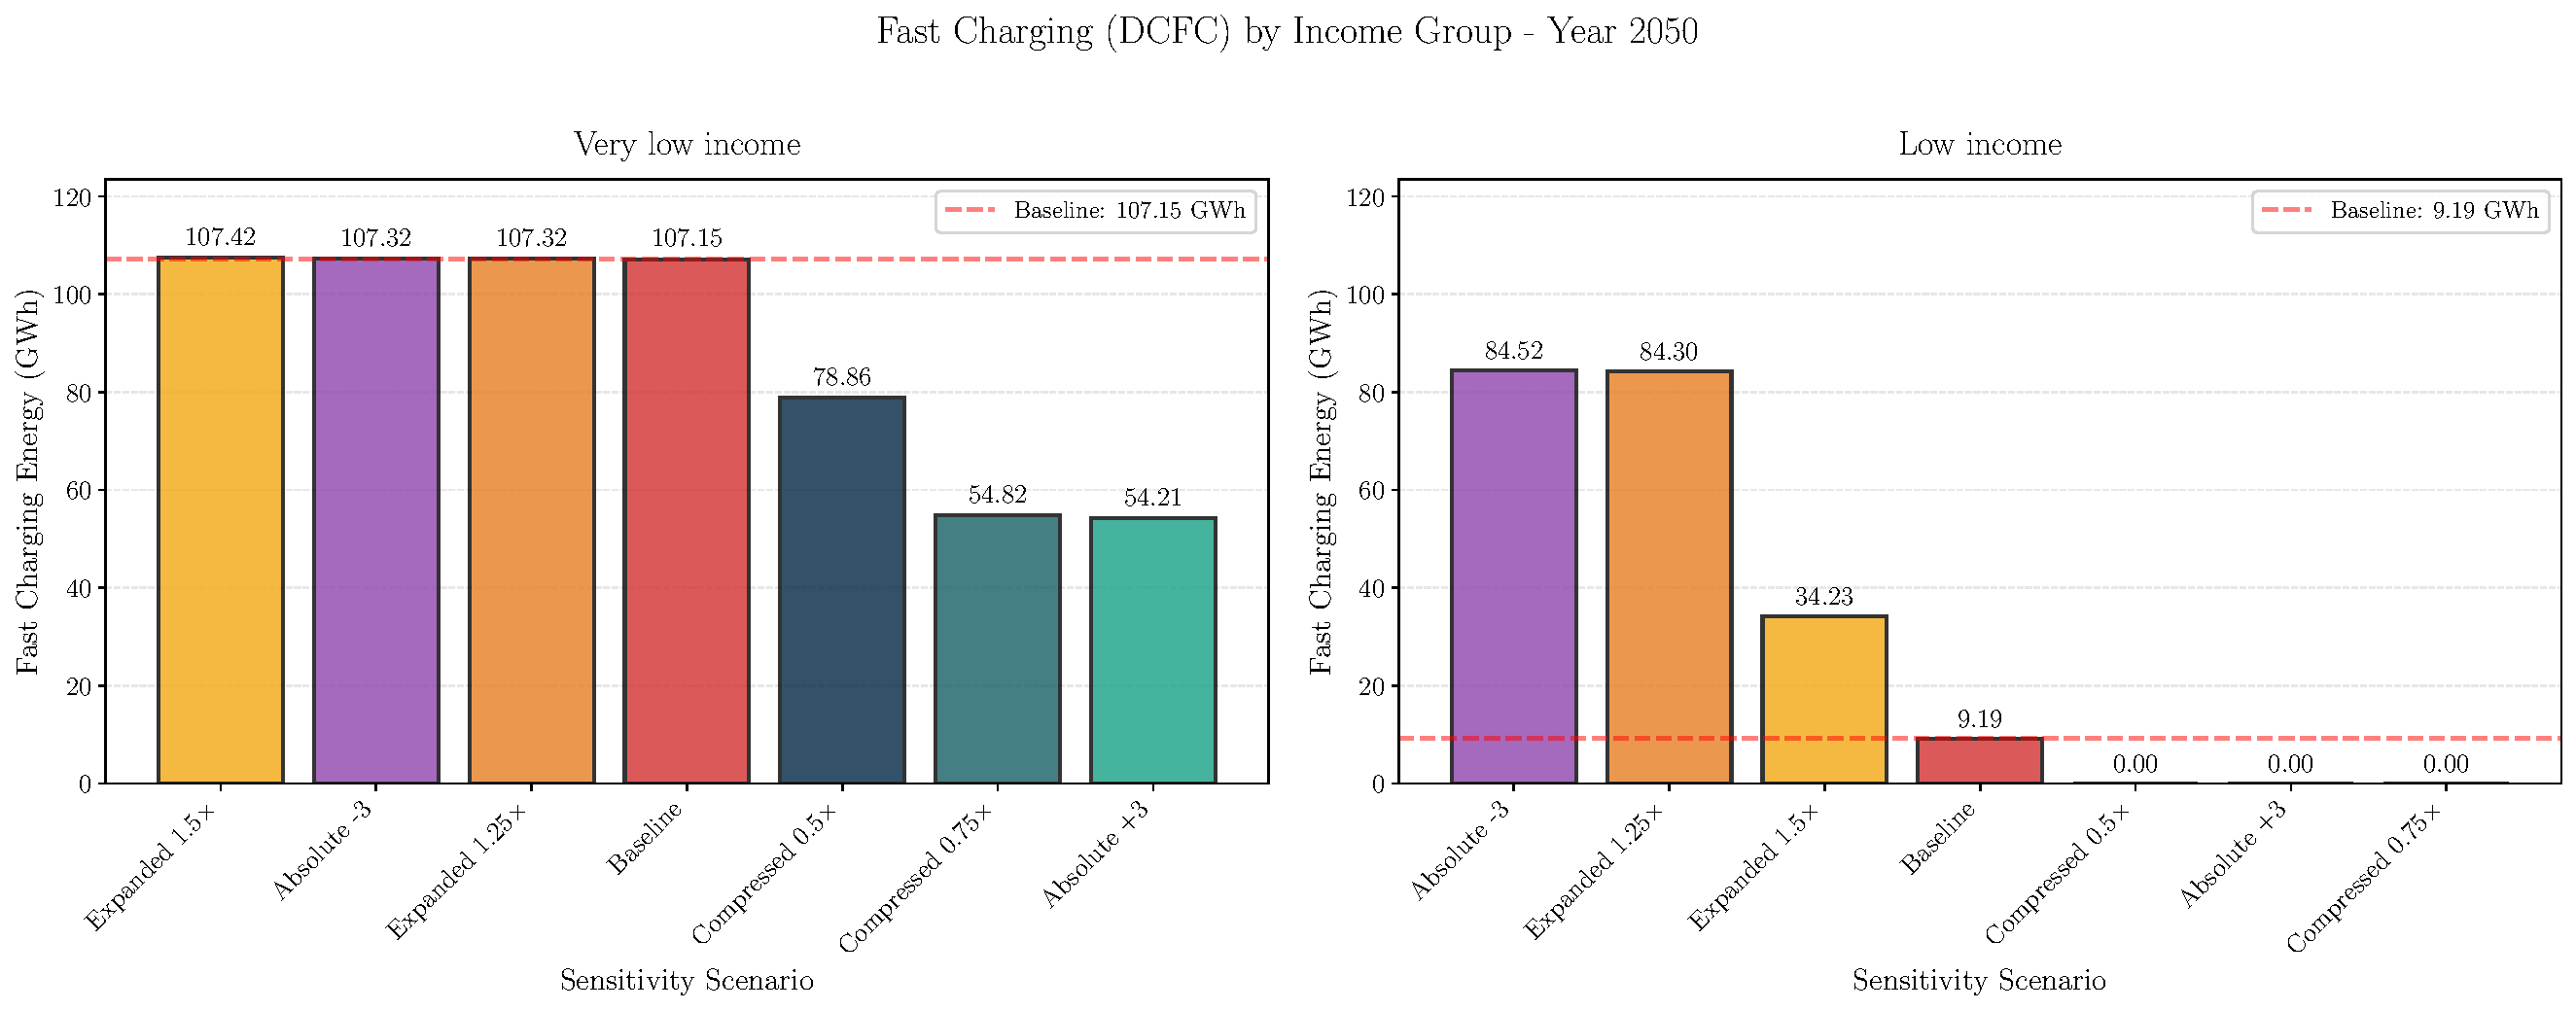
\includegraphics[width=0.9\textwidth]{graphics/SA_fast_charging_low_income_comparison.pdf}
    \captionsetup{labelfont={color=authorblue}, textfont={color=authorblue}}

    \caption{Charged energy by fast chargers in 2050 for different VoT scenarios. \textit{Left:} \textit{Very low income} consumer group. \textit{Right:} \textit{Low income} consumer group.} \label{fig: VoT_fastcharg_4}
\end{figure} 

This observation is coherent with observations presented in the \textit{Results} section, in particular, Section 4.1. where we show differences of fast charger utilization through variation in levels of service induced by charging infrastructure densification. There, as well as in these VoT scenarios, we observe how the term $\mathrm{VoT} \times \mathrm{level~of~service}$ influences charger-type utilization across income groups.    
\\
\color{reviewergrey}
\subsubsection*{3. Other Inputs with Missing Context - Again, monetary budgets for vehicle purchases (Sec 3.3.1) are derived from UK statistics. The paper provides no justification for why UK household expenditure on cars is a valid proxy for households in the Basque Country. Also, the paper does not explain why the initial charging shares (e.g., 88\% at home) from a 2019 study (Baresch and Moser, 2019) and the average fuel price (Martin et al., 2023) are applicable or comparable to the study region. Lastly, the 30\% assumption for e-mobility's share of new grid capacity (Sec 3.3.3) is a critical model constraint, yet it is based on a single 2017 report's "relative share" with minimal justification. The authors should provide clear and valid reasonings why certain assumptions are used.}
\color{authorblue}
\noindent \textcolor{authorblue}{\textbf{Author's response:}}  Thank you for highlighting these limitations. As we lack local information and empirical data, we have to draw from empirical observations from other studies. Part of this is the linear relation between the income and expenditure for purchases of vehicles. We do not directly draw values from this study but use it to justify the linear relation introduced in the “Purchase frequency” value. We apologize for the misunderstanding and improve the wording of the statement in the text. 

We use initial charging shares of 88\% to approximate existing home charging capacities. We cite the Austrian publication as this directly addresses the current state of how much of the charging demand is covered by home chargers \cite{BARESCH2019388}. This value is also in a range of the approximation that has been made for Spain by the Technology Collaboration Program [85\% in the report \citep{HEVTCP2024}]. A recent report by the IEA reports that the shares of home charging are globally similar --- in the UK at around 93\% and Norway 82\% \citep{IEA2024}. Therefore, we believe that 88\% is an acceptable approximation for Spain. 

Concerning the comment on available grid capacity, this limitation is not imposed in the model. We recognize that this sentence is misleading in this context. We have assumed a maximum of 30\% of yearly expansion which is consistent with early-stage charging infrastructure expansion and this is used as an upper bound for the expansion speed for charging infrastructure capacities. We apologize for the misunderstanding and included a statement on this in the Methodology description (see Section 3.3.3).
\color{reviewergrey}
\subsubsection*{4. Contradiction in "Fueling Detour Time" Approach - The methodology used to answer RQ1 assumes a "spatially even distribution" from the beginning, modeling the region as a rectangle. The authors' justification for this (Sec. 3.4) is that "a spatially even distribution \dots is a necessity" for a future 100\% BEV state "to be equally accessible for all." This justification is highly problematic and contradicts the RQ1. Instead of identifying an optimal spatial distribution, the model is imposing that chargers are spread out evenly. In a way, the real-world problem describing that population lives in un-even clusters and income groups are not being accounted for properly.}
\color{authorblue}
\noindent \textcolor{authorblue}{\textbf{Author's response:}} Thank you for noticing this! We agree that the current formulation using “spatial distribution” does not match the analysis under the made assumptions. We have adapted the formulation of the research question slightly and now use the wording of “spatial density” to reflect the analysis more accurately. This does not fundamentally change the research question but refines the wording. Now it is changed to “To what extent does the spatial density of public charging infrastructure influence battery-electric vehicle adoption across consumers with different income levels?” 
As we model the region on NUTS-2 level, we model the distribution without details on the exact relative location to BEV passenger drivers. On the one hand, we thereby neglect the heterogeneity of the built environment, driving distances and relative locations of charger allocations to households of different income types. On the other hand, we gain the computational efficiency at the NUTS-2 geographic scope through being able to model the BEV adoption, optimal investments in fueling/charging infrastructure together with the improved level of service by charging infrastructure expansion. \\
\color{reviewergrey}
\subsubsection*{5. Mismatch in Measuring Spill-Over Effect - The "spill-over effect" described in the literature is primarily a psychological phenomenon (i.e., seeing chargers in neighboring regions reduces a consumer's range anxiety, making them more likely to adopt). The paper's techno-economic model does not capture this psychological effect. The model's way to measure a "spill-over" is oversimplified: a commuter from Region A drives to Region B, charges there, and thus "frees up" capacity back in Region A. This could be why a 30\% increase in local capacity yields only a 1.3\% impact on the BEV adoption in a neighboring region, which can be argued insignificant in real-world application.}
\color{authorblue}
\noindent \textcolor{authorblue}{\textbf{Author's response:}}
Thank you for raising this issue. We acknowledge this concern and  we have reviewed the formal definition of \say{Spillover effect}. We checked again and have found that this term is broadly used. In the Limitation section (Section 5.2.2.), we discuss that our approach exclusively addresses the techno-economic dimension of the spillover effect. 

A recent article published by the European Commission defines the \say{spillover} effect in the following quote: \say{The impacts that activities in one sector, region or country have on other sectors, regions or countries are called spillover effects.} An inherent part of this is that the activities in one sector, region or country are not aimed to impact other sectors, regions or countries. Our work analyzes the impact of increased expansion in one region, that is only aimed to support the fleet locally, to the adoption of BEVs in the neighboring regions. Based on this, we decide to keep the wording. We have included a clear definition of the spillover we aim to measure at the first mention of the word (see Section 1). \\\\
\color{reviewergrey}
\textbf{In summary, I believe the paper's research questions are excellent, but its core findings are undermined by the combinations of these issues, making it difficult to have confidence in the model's key outputs, such as the specific charging preferences by income class or the magnitude of spill-over effects. I strongly recommend the authors acknowledge the full extent of these data limitations and their impact on the results much more prominently in the Discussion and Conclusion sections. In addition, they must justify why these data proxies are at all appropriate for the Basque Country, providing supporting evidence of comparability (e.g., in mode share, geography, or economic structure). Lastly, the authors should address and properly justify why these critical assumptions (e.g., all income groups travel identically, and a spatially even distribution of charger availability is a necessity) do not invalidate the novelty and contributions of the paper. } \\\\
\color{authorblue}
\noindent \textcolor{authorblue}{\textbf{Author's response:}} We would like to thank you for the time you dedicated to reviewing our manuscript and for the constructive comments provided. Throughout the revision process, we have focused on addressing the concerns regarding the robustness of our results and conclusions. We believe that the expanded presentation of sensitivity analyses for key parameters, along with the improved descriptions and data-based justifications, adequately addresses the concerns raised about the contributions of the paper.

\color{black}
\newpage
\fancyhead[L]{References}
\bibliographystyle{elsarticle-harv}
\bibliography{literature}

\end{document}